\documentclass[twoside]{book}

% Packages required by doxygen
\usepackage{fixltx2e}
\usepackage{calc}
\usepackage{doxygen}
\usepackage[export]{adjustbox} % also loads graphicx
\usepackage{graphicx}
\usepackage[utf8]{inputenc}
\usepackage{makeidx}
\usepackage{multicol}
\usepackage{multirow}
\PassOptionsToPackage{warn}{textcomp}
\usepackage{textcomp}
\usepackage[nointegrals]{wasysym}
\usepackage[table]{xcolor}

% Font selection
\usepackage[T1]{fontenc}
\usepackage[scaled=.90]{helvet}
\usepackage{courier}
\usepackage{amssymb}
\usepackage{sectsty}
\renewcommand{\familydefault}{\sfdefault}
\allsectionsfont{%
  \fontseries{bc}\selectfont%
  \color{darkgray}%
}
\renewcommand{\DoxyLabelFont}{%
  \fontseries{bc}\selectfont%
  \color{darkgray}%
}
\newcommand{\+}{\discretionary{\mbox{\scriptsize$\hookleftarrow$}}{}{}}

% Page & text layout
\usepackage{geometry}
\geometry{%
  a4paper,%
  top=2.5cm,%
  bottom=2.5cm,%
  left=2.5cm,%
  right=2.5cm%
}
\tolerance=750
\hfuzz=15pt
\hbadness=750
\setlength{\emergencystretch}{15pt}
\setlength{\parindent}{0cm}
\setlength{\parskip}{3ex plus 2ex minus 2ex}
\makeatletter
\renewcommand{\paragraph}{%
  \@startsection{paragraph}{4}{0ex}{-1.0ex}{1.0ex}{%
    \normalfont\normalsize\bfseries\SS@parafont%
  }%
}
\renewcommand{\subparagraph}{%
  \@startsection{subparagraph}{5}{0ex}{-1.0ex}{1.0ex}{%
    \normalfont\normalsize\bfseries\SS@subparafont%
  }%
}
\makeatother

% Headers & footers
\usepackage{fancyhdr}
\pagestyle{fancyplain}
\fancyhead[LE]{\fancyplain{}{\bfseries\thepage}}
\fancyhead[CE]{\fancyplain{}{}}
\fancyhead[RE]{\fancyplain{}{\bfseries\leftmark}}
\fancyhead[LO]{\fancyplain{}{\bfseries\rightmark}}
\fancyhead[CO]{\fancyplain{}{}}
\fancyhead[RO]{\fancyplain{}{\bfseries\thepage}}
\fancyfoot[LE]{\fancyplain{}{}}
\fancyfoot[CE]{\fancyplain{}{}}
\fancyfoot[RE]{\fancyplain{}{\bfseries\scriptsize Generated by Doxygen }}
\fancyfoot[LO]{\fancyplain{}{\bfseries\scriptsize Generated by Doxygen }}
\fancyfoot[CO]{\fancyplain{}{}}
\fancyfoot[RO]{\fancyplain{}{}}
\renewcommand{\footrulewidth}{0.4pt}
\renewcommand{\chaptermark}[1]{%
  \markboth{#1}{}%
}
\renewcommand{\sectionmark}[1]{%
  \markright{\thesection\ #1}%
}

% Indices & bibliography
\usepackage{natbib}
\usepackage[titles]{tocloft}
\setcounter{tocdepth}{3}
\setcounter{secnumdepth}{5}
\makeindex

% Hyperlinks (required, but should be loaded last)
\usepackage{ifpdf}
\ifpdf
  \usepackage[pdftex,pagebackref=true]{hyperref}
\else
  \usepackage[ps2pdf,pagebackref=true]{hyperref}
\fi
\hypersetup{%
  colorlinks=true,%
  linkcolor=blue,%
  citecolor=blue,%
  unicode%
}

% Custom commands
\newcommand{\clearemptydoublepage}{%
  \newpage{\pagestyle{empty}\cleardoublepage}%
}

\usepackage{caption}
\captionsetup{labelsep=space,justification=centering,font={bf},singlelinecheck=off,skip=4pt,position=top}

%===== C O N T E N T S =====

\begin{document}

% Titlepage & ToC
\hypersetup{pageanchor=false,
             bookmarksnumbered=true,
             pdfencoding=unicode
            }
\pagenumbering{roman}
\begin{titlepage}
\vspace*{7cm}
\begin{center}%
{\Large Smart Waste }\\
\vspace*{1cm}
{\large Generated by Doxygen 1.8.11}\\
\end{center}
\end{titlepage}
\clearemptydoublepage
\tableofcontents
\clearemptydoublepage
\pagenumbering{arabic}
\hypersetup{pageanchor=true}

%--- Begin generated contents ---
\chapter{Namespace Index}
\section{Namespace List}
Here is a list of all namespaces with brief descriptions\+:\begin{DoxyCompactList}
\item\contentsline{section}{\hyperlink{namespaceUtils}{Utils} }{\pageref{namespaceUtils}}{}
\end{DoxyCompactList}

\chapter{Class Index}
\section{Class List}
Here are the classes, structs, unions and interfaces with brief descriptions\+:\begin{DoxyCompactList}
\item\contentsline{section}{\hyperlink{classConnection}{Connection} }{\pageref{classConnection}}{}
\item\contentsline{section}{\hyperlink{classEdge}{Edge$<$ T $>$} }{\pageref{classEdge}}{}
\item\contentsline{section}{\hyperlink{classEdgeType}{Edge\+Type} }{\pageref{classEdgeType}}{}
\item\contentsline{section}{\hyperlink{classGraph}{Graph$<$ T $>$} }{\pageref{classGraph}}{}
\item\contentsline{section}{\hyperlink{classGraphViewer}{Graph\+Viewer} }{\pageref{classGraphViewer}}{}
\item\contentsline{section}{\hyperlink{classSmartWaste}{Smart\+Waste} }{\pageref{classSmartWaste}}{}
\item\contentsline{section}{\hyperlink{classVertex}{Vertex$<$ T $>$} }{\pageref{classVertex}}{}
\item\contentsline{section}{\hyperlink{structvertex__greater__than}{vertex\+\_\+greater\+\_\+than$<$ T $>$} }{\pageref{structvertex__greater__than}}{}
\end{DoxyCompactList}

\chapter{File Index}
\section{File List}
Here is a list of all files with brief descriptions\+:\begin{DoxyCompactList}
\item\contentsline{section}{/home/ana/\+Dropbox/faculdade/2ano/2semestre/\+C\+A\+L/\+Smart\+Waste/src/\hyperlink{connection_8cpp}{connection.\+cpp} }{\pageref{connection_8cpp}}{}
\item\contentsline{section}{/home/ana/\+Dropbox/faculdade/2ano/2semestre/\+C\+A\+L/\+Smart\+Waste/src/\hyperlink{connection_8h}{connection.\+h} }{\pageref{connection_8h}}{}
\item\contentsline{section}{/home/ana/\+Dropbox/faculdade/2ano/2semestre/\+C\+A\+L/\+Smart\+Waste/src/\hyperlink{edgetype_8h}{edgetype.\+h} }{\pageref{edgetype_8h}}{}
\item\contentsline{section}{/home/ana/\+Dropbox/faculdade/2ano/2semestre/\+C\+A\+L/\+Smart\+Waste/src/\hyperlink{Graph_8h}{Graph.\+h} }{\pageref{Graph_8h}}{}
\item\contentsline{section}{/home/ana/\+Dropbox/faculdade/2ano/2semestre/\+C\+A\+L/\+Smart\+Waste/src/\hyperlink{graphviewer_8cpp}{graphviewer.\+cpp} }{\pageref{graphviewer_8cpp}}{}
\item\contentsline{section}{/home/ana/\+Dropbox/faculdade/2ano/2semestre/\+C\+A\+L/\+Smart\+Waste/src/\hyperlink{graphviewer_8h}{graphviewer.\+h} }{\pageref{graphviewer_8h}}{}
\item\contentsline{section}{/home/ana/\+Dropbox/faculdade/2ano/2semestre/\+C\+A\+L/\+Smart\+Waste/src/\hyperlink{main_8cpp}{main.\+cpp} }{\pageref{main_8cpp}}{}
\item\contentsline{section}{/home/ana/\+Dropbox/faculdade/2ano/2semestre/\+C\+A\+L/\+Smart\+Waste/src/\hyperlink{SmartWaste_8cpp}{Smart\+Waste.\+cpp} }{\pageref{SmartWaste_8cpp}}{}
\item\contentsline{section}{/home/ana/\+Dropbox/faculdade/2ano/2semestre/\+C\+A\+L/\+Smart\+Waste/src/\hyperlink{SmartWaste_8h}{Smart\+Waste.\+h} }{\pageref{SmartWaste_8h}}{}
\item\contentsline{section}{/home/ana/\+Dropbox/faculdade/2ano/2semestre/\+C\+A\+L/\+Smart\+Waste/src/\hyperlink{Utils_8cpp}{Utils.\+cpp} }{\pageref{Utils_8cpp}}{}
\item\contentsline{section}{/home/ana/\+Dropbox/faculdade/2ano/2semestre/\+C\+A\+L/\+Smart\+Waste/src/\hyperlink{Utils_8h}{Utils.\+h} }{\pageref{Utils_8h}}{}
\end{DoxyCompactList}

\chapter{Namespace Documentation}
\hypertarget{namespaceUtils}{}\section{Utils Namespace Reference}
\label{namespaceUtils}\index{Utils@{Utils}}
\subsection*{Functions}
\begin{DoxyCompactItemize}
\item 
void \hyperlink{namespaceUtils_a71478c18b3a127080dcb2bb1717aff47}{do\+Sleep} (int s)
\begin{DoxyCompactList}\small\item\em Do sleep according to the operating system. \end{DoxyCompactList}\item 
int \hyperlink{namespaceUtils_a030e2d39f8dc5367f990ae1ae0743aa7}{distance} (int y1, int x1, int y2, int x2)
\begin{DoxyCompactList}\small\item\em calculate distance \end{DoxyCompactList}\item 
std\+::vector$<$ std\+::string $>$ \hyperlink{namespaceUtils_ad0e14037565bd51622c72b283730a1fc}{split\+Line} (std\+::string str, char c)
\begin{DoxyCompactList}\small\item\em split one line in vector of strings \end{DoxyCompactList}\end{DoxyCompactItemize}


\subsection{Function Documentation}
\index{Utils@{Utils}!distance@{distance}}
\index{distance@{distance}!Utils@{Utils}}
\subsubsection[{\texorpdfstring{distance(int y1, int x1, int y2, int x2)}{distance(int y1, int x1, int y2, int x2)}}]{\setlength{\rightskip}{0pt plus 5cm}int Utils\+::distance (
\begin{DoxyParamCaption}
\item[{int}]{y1, }
\item[{int}]{x1, }
\item[{int}]{y2, }
\item[{int}]{x2}
\end{DoxyParamCaption}
)}\hypertarget{namespaceUtils_a030e2d39f8dc5367f990ae1ae0743aa7}{}\label{namespaceUtils_a030e2d39f8dc5367f990ae1ae0743aa7}


calculate distance 


\begin{DoxyParams}{Parameters}
{\em x1} & \\
\hline
{\em x2} & \\
\hline
{\em y1} & \\
\hline
{\em y2} & \\
\hline
\end{DoxyParams}
\begin{DoxyReturn}{Returns}
distance 
\end{DoxyReturn}
\index{Utils@{Utils}!do\+Sleep@{do\+Sleep}}
\index{do\+Sleep@{do\+Sleep}!Utils@{Utils}}
\subsubsection[{\texorpdfstring{do\+Sleep(int s)}{doSleep(int s)}}]{\setlength{\rightskip}{0pt plus 5cm}void Utils\+::do\+Sleep (
\begin{DoxyParamCaption}
\item[{int}]{s}
\end{DoxyParamCaption}
)}\hypertarget{namespaceUtils_a71478c18b3a127080dcb2bb1717aff47}{}\label{namespaceUtils_a71478c18b3a127080dcb2bb1717aff47}


Do sleep according to the operating system. 


\begin{DoxyParams}{Parameters}
{\em s} & \\
\hline
\end{DoxyParams}
\index{Utils@{Utils}!split\+Line@{split\+Line}}
\index{split\+Line@{split\+Line}!Utils@{Utils}}
\subsubsection[{\texorpdfstring{split\+Line(std\+::string str, char c)}{splitLine(std::string str, char c)}}]{\setlength{\rightskip}{0pt plus 5cm}std\+::vector$<$ std\+::string $>$ Utils\+::split\+Line (
\begin{DoxyParamCaption}
\item[{std\+::string}]{str, }
\item[{char}]{c}
\end{DoxyParamCaption}
)}\hypertarget{namespaceUtils_ad0e14037565bd51622c72b283730a1fc}{}\label{namespaceUtils_ad0e14037565bd51622c72b283730a1fc}


split one line in vector of strings 


\begin{DoxyParams}{Parameters}
{\em str} & \\
\hline
{\em c} & \\
\hline
\end{DoxyParams}
\begin{DoxyReturn}{Returns}
vector of strings 
\end{DoxyReturn}

\chapter{Class Documentation}
\hypertarget{classConnection}{}\section{Connection Class Reference}
\label{classConnection}\index{Connection@{Connection}}


{\ttfamily \#include $<$connection.\+h$>$}

\subsection*{Public Member Functions}
\begin{DoxyCompactItemize}
\item 
\hyperlink{classConnection_a8089476d48ba545f44e691cd4bd0278d}{Connection} (short port)
\item 
bool \hyperlink{classConnection_a4b9f6db1fb42fc9857f829fa0bc52e6e}{send\+Msg} (string msg)
\item 
string \hyperlink{classConnection_a1df16b436751b686d96c24ca0c498659}{read\+Line} ()
\end{DoxyCompactItemize}
\subsection*{Private Attributes}
\begin{DoxyCompactItemize}
\item 
S\+O\+C\+K\+ET \hyperlink{classConnection_a50ca7c17a64836ca25a1fe9953cc6cf6}{sock}
\end{DoxyCompactItemize}


\subsection{Constructor \& Destructor Documentation}
\index{Connection@{Connection}!Connection@{Connection}}
\index{Connection@{Connection}!Connection@{Connection}}
\subsubsection[{\texorpdfstring{Connection(short port)}{Connection(short port)}}]{\setlength{\rightskip}{0pt plus 5cm}Connection\+::\+Connection (
\begin{DoxyParamCaption}
\item[{short}]{port}
\end{DoxyParamCaption}
)}\hypertarget{classConnection_a8089476d48ba545f44e691cd4bd0278d}{}\label{classConnection_a8089476d48ba545f44e691cd4bd0278d}


Here is the call graph for this function\+:
\nopagebreak
\begin{figure}[H]
\begin{center}
\leavevmode
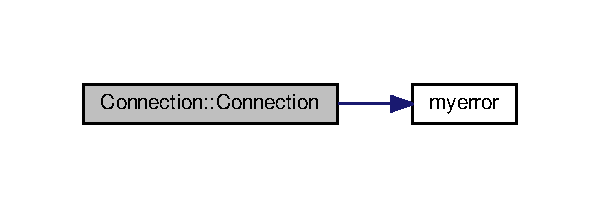
\includegraphics[width=288pt]{classConnection_a8089476d48ba545f44e691cd4bd0278d_cgraph}
\end{center}
\end{figure}




\subsection{Member Function Documentation}
\index{Connection@{Connection}!read\+Line@{read\+Line}}
\index{read\+Line@{read\+Line}!Connection@{Connection}}
\subsubsection[{\texorpdfstring{read\+Line()}{readLine()}}]{\setlength{\rightskip}{0pt plus 5cm}string Connection\+::read\+Line (
\begin{DoxyParamCaption}
{}
\end{DoxyParamCaption}
)}\hypertarget{classConnection_a1df16b436751b686d96c24ca0c498659}{}\label{classConnection_a1df16b436751b686d96c24ca0c498659}
\index{Connection@{Connection}!send\+Msg@{send\+Msg}}
\index{send\+Msg@{send\+Msg}!Connection@{Connection}}
\subsubsection[{\texorpdfstring{send\+Msg(string msg)}{sendMsg(string msg)}}]{\setlength{\rightskip}{0pt plus 5cm}bool Connection\+::send\+Msg (
\begin{DoxyParamCaption}
\item[{string}]{msg}
\end{DoxyParamCaption}
)}\hypertarget{classConnection_a4b9f6db1fb42fc9857f829fa0bc52e6e}{}\label{classConnection_a4b9f6db1fb42fc9857f829fa0bc52e6e}


Here is the call graph for this function\+:
\nopagebreak
\begin{figure}[H]
\begin{center}
\leavevmode
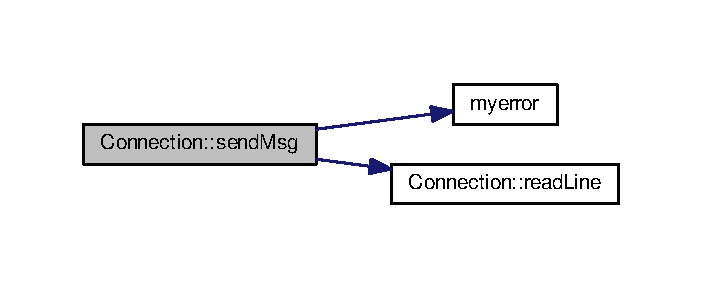
\includegraphics[width=337pt]{classConnection_a4b9f6db1fb42fc9857f829fa0bc52e6e_cgraph}
\end{center}
\end{figure}




\subsection{Member Data Documentation}
\index{Connection@{Connection}!sock@{sock}}
\index{sock@{sock}!Connection@{Connection}}
\subsubsection[{\texorpdfstring{sock}{sock}}]{\setlength{\rightskip}{0pt plus 5cm}S\+O\+C\+K\+ET Connection\+::sock\hspace{0.3cm}{\ttfamily [private]}}\hypertarget{classConnection_a50ca7c17a64836ca25a1fe9953cc6cf6}{}\label{classConnection_a50ca7c17a64836ca25a1fe9953cc6cf6}


The documentation for this class was generated from the following files\+:\begin{DoxyCompactItemize}
\item 
/home/ana/\+Dropbox/faculdade/2ano/2semestre/\+C\+A\+L/\+Smart\+Waste/src/\hyperlink{connection_8h}{connection.\+h}\item 
/home/ana/\+Dropbox/faculdade/2ano/2semestre/\+C\+A\+L/\+Smart\+Waste/src/\hyperlink{connection_8cpp}{connection.\+cpp}\end{DoxyCompactItemize}

\hypertarget{classEdge}{}\section{Edge$<$ T $>$ Class Template Reference}
\label{classEdge}\index{Edge$<$ T $>$@{Edge$<$ T $>$}}


{\ttfamily \#include $<$Graph.\+h$>$}

\subsection*{Public Member Functions}
\begin{DoxyCompactItemize}
\item 
\hyperlink{classEdge_a96686534f9eefc8cce07582f7f38369b}{Edge} (T i, \hyperlink{classVertex}{Vertex}$<$ T $>$ $\ast$d, double w)
\item 
T \hyperlink{classEdge_a9cfd65d4ac2da66e35350e6ad7ab531e}{get\+Info} ()
\end{DoxyCompactItemize}
\subsection*{Private Attributes}
\begin{DoxyCompactItemize}
\item 
\hyperlink{classVertex}{Vertex}$<$ T $>$ $\ast$ \hyperlink{classEdge_ae4d65678b91bd9d814af4720ad87cd0c}{dest}
\item 
double \hyperlink{classEdge_af188b57b604f0d65e2da48733bd76426}{weight}
\item 
T \hyperlink{classEdge_a3c76337d535f346456b825b3cbc88b14}{info}
\end{DoxyCompactItemize}
\subsection*{Friends}
\begin{DoxyCompactItemize}
\item 
class \hyperlink{classEdge_aefa9b76cd57411c5354e5620dc2d84dd}{Graph$<$ T $>$}
\item 
class \hyperlink{classEdge_a2e120a12dec663fa334633b4f26cbed8}{Vertex$<$ T $>$}
\end{DoxyCompactItemize}


\subsection{Constructor \& Destructor Documentation}
\index{Edge@{Edge}!Edge@{Edge}}
\index{Edge@{Edge}!Edge@{Edge}}
\subsubsection[{\texorpdfstring{Edge(\+T i, Vertex$<$ T $>$ $\ast$d, double w)}{Edge(T i, Vertex< T > *d, double w)}}]{\setlength{\rightskip}{0pt plus 5cm}template$<$class T $>$ {\bf Edge}$<$ T $>$\+::{\bf Edge} (
\begin{DoxyParamCaption}
\item[{T}]{i, }
\item[{{\bf Vertex}$<$ T $>$ $\ast$}]{d, }
\item[{double}]{w}
\end{DoxyParamCaption}
)}\hypertarget{classEdge_a96686534f9eefc8cce07582f7f38369b}{}\label{classEdge_a96686534f9eefc8cce07582f7f38369b}


\subsection{Member Function Documentation}
\index{Edge@{Edge}!get\+Info@{get\+Info}}
\index{get\+Info@{get\+Info}!Edge@{Edge}}
\subsubsection[{\texorpdfstring{get\+Info()}{getInfo()}}]{\setlength{\rightskip}{0pt plus 5cm}template$<$class T $>$ T {\bf Edge}$<$ T $>$\+::get\+Info (
\begin{DoxyParamCaption}
{}
\end{DoxyParamCaption}
)}\hypertarget{classEdge_a9cfd65d4ac2da66e35350e6ad7ab531e}{}\label{classEdge_a9cfd65d4ac2da66e35350e6ad7ab531e}


\subsection{Friends And Related Function Documentation}
\index{Edge@{Edge}!Graph$<$ T $>$@{Graph$<$ T $>$}}
\index{Graph$<$ T $>$@{Graph$<$ T $>$}!Edge@{Edge}}
\subsubsection[{\texorpdfstring{Graph$<$ T $>$}{Graph< T >}}]{\setlength{\rightskip}{0pt plus 5cm}template$<$class T$>$ friend class {\bf Graph}$<$ T $>$\hspace{0.3cm}{\ttfamily [friend]}}\hypertarget{classEdge_aefa9b76cd57411c5354e5620dc2d84dd}{}\label{classEdge_aefa9b76cd57411c5354e5620dc2d84dd}
\index{Edge@{Edge}!Vertex$<$ T $>$@{Vertex$<$ T $>$}}
\index{Vertex$<$ T $>$@{Vertex$<$ T $>$}!Edge@{Edge}}
\subsubsection[{\texorpdfstring{Vertex$<$ T $>$}{Vertex< T >}}]{\setlength{\rightskip}{0pt plus 5cm}template$<$class T$>$ friend class {\bf Vertex}$<$ T $>$\hspace{0.3cm}{\ttfamily [friend]}}\hypertarget{classEdge_a2e120a12dec663fa334633b4f26cbed8}{}\label{classEdge_a2e120a12dec663fa334633b4f26cbed8}


\subsection{Member Data Documentation}
\index{Edge@{Edge}!dest@{dest}}
\index{dest@{dest}!Edge@{Edge}}
\subsubsection[{\texorpdfstring{dest}{dest}}]{\setlength{\rightskip}{0pt plus 5cm}template$<$class T$>$ {\bf Vertex}$<$T$>$$\ast$ {\bf Edge}$<$ T $>$\+::dest\hspace{0.3cm}{\ttfamily [private]}}\hypertarget{classEdge_ae4d65678b91bd9d814af4720ad87cd0c}{}\label{classEdge_ae4d65678b91bd9d814af4720ad87cd0c}
\index{Edge@{Edge}!info@{info}}
\index{info@{info}!Edge@{Edge}}
\subsubsection[{\texorpdfstring{info}{info}}]{\setlength{\rightskip}{0pt plus 5cm}template$<$class T$>$ T {\bf Edge}$<$ T $>$\+::info\hspace{0.3cm}{\ttfamily [private]}}\hypertarget{classEdge_a3c76337d535f346456b825b3cbc88b14}{}\label{classEdge_a3c76337d535f346456b825b3cbc88b14}
\index{Edge@{Edge}!weight@{weight}}
\index{weight@{weight}!Edge@{Edge}}
\subsubsection[{\texorpdfstring{weight}{weight}}]{\setlength{\rightskip}{0pt plus 5cm}template$<$class T$>$ double {\bf Edge}$<$ T $>$\+::weight\hspace{0.3cm}{\ttfamily [private]}}\hypertarget{classEdge_af188b57b604f0d65e2da48733bd76426}{}\label{classEdge_af188b57b604f0d65e2da48733bd76426}


The documentation for this class was generated from the following file\+:\begin{DoxyCompactItemize}
\item 
/home/ana/\+Dropbox/faculdade/2ano/2semestre/\+C\+A\+L/\+Smart\+Waste/src/\hyperlink{Graph_8h}{Graph.\+h}\end{DoxyCompactItemize}

\hypertarget{classEdgeType}{}\section{Edge\+Type Class Reference}
\label{classEdgeType}\index{Edge\+Type@{Edge\+Type}}


{\ttfamily \#include $<$edgetype.\+h$>$}

\subsection*{Static Public Attributes}
\begin{DoxyCompactItemize}
\item 
static const int \hyperlink{classEdgeType_a6533cc56d05c288a550b9980b66c9317}{U\+N\+D\+I\+R\+E\+C\+T\+ED} = 0
\item 
static const int \hyperlink{classEdgeType_a903017a534f2818c2d17145e4ae0321c}{D\+I\+R\+E\+C\+T\+ED} = 1
\end{DoxyCompactItemize}


\subsection{Detailed Description}
Classe que enumera os tipos de arestas. Usar \hyperlink{classEdgeType_a6533cc56d05c288a550b9980b66c9317}{Edge\+Type.\+U\+N\+D\+I\+R\+E\+C\+T\+ED} para uma aresta sem direcção, ou \hyperlink{classEdgeType_a903017a534f2818c2d17145e4ae0321c}{Edge\+Type.\+D\+I\+R\+E\+C\+T\+ED} para uma aresta dirigida. 

\subsection{Member Data Documentation}
\index{Edge\+Type@{Edge\+Type}!D\+I\+R\+E\+C\+T\+ED@{D\+I\+R\+E\+C\+T\+ED}}
\index{D\+I\+R\+E\+C\+T\+ED@{D\+I\+R\+E\+C\+T\+ED}!Edge\+Type@{Edge\+Type}}
\subsubsection[{\texorpdfstring{D\+I\+R\+E\+C\+T\+ED}{DIRECTED}}]{\setlength{\rightskip}{0pt plus 5cm}const int Edge\+Type\+::\+D\+I\+R\+E\+C\+T\+ED = 1\hspace{0.3cm}{\ttfamily [static]}}\hypertarget{classEdgeType_a903017a534f2818c2d17145e4ae0321c}{}\label{classEdgeType_a903017a534f2818c2d17145e4ae0321c}
\index{Edge\+Type@{Edge\+Type}!U\+N\+D\+I\+R\+E\+C\+T\+ED@{U\+N\+D\+I\+R\+E\+C\+T\+ED}}
\index{U\+N\+D\+I\+R\+E\+C\+T\+ED@{U\+N\+D\+I\+R\+E\+C\+T\+ED}!Edge\+Type@{Edge\+Type}}
\subsubsection[{\texorpdfstring{U\+N\+D\+I\+R\+E\+C\+T\+ED}{UNDIRECTED}}]{\setlength{\rightskip}{0pt plus 5cm}const int Edge\+Type\+::\+U\+N\+D\+I\+R\+E\+C\+T\+ED = 0\hspace{0.3cm}{\ttfamily [static]}}\hypertarget{classEdgeType_a6533cc56d05c288a550b9980b66c9317}{}\label{classEdgeType_a6533cc56d05c288a550b9980b66c9317}


The documentation for this class was generated from the following file\+:\begin{DoxyCompactItemize}
\item 
/home/ana/\+Dropbox/faculdade/2ano/2semestre/\+C\+A\+L/\+Smart\+Waste/src/\hyperlink{edgetype_8h}{edgetype.\+h}\end{DoxyCompactItemize}

\hypertarget{classGraph}{}\section{Graph$<$ T $>$ Class Template Reference}
\label{classGraph}\index{Graph$<$ T $>$@{Graph$<$ T $>$}}


{\ttfamily \#include $<$Graph.\+h$>$}



Collaboration diagram for Graph$<$ T $>$\+:
\nopagebreak
\begin{figure}[H]
\begin{center}
\leavevmode
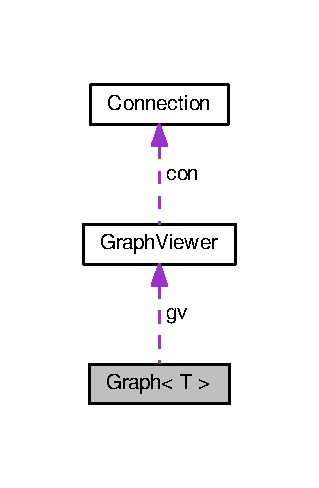
\includegraphics[width=153pt]{classGraph__coll__graph}
\end{center}
\end{figure}
\subsection*{Public Member Functions}
\begin{DoxyCompactItemize}
\item 
\hyperlink{classGraph_acda25b82a1565955306b44ae01660349}{Graph} (\hyperlink{classGraphViewer}{Graph\+Viewer} $\ast$)
\item 
bool \hyperlink{classGraph_a18f099535183b37aef90bb55f4669e65}{add\+Vertex} (const T \&in, std\+::pair$<$ double, double $>$ coords)
\item 
void \hyperlink{classGraph_af720eb3f731732a2fafc40141f4d41c3}{add\+Edge} (const T \&edge\+Id, const string \&road\+Name, const T \&sourc, const T \&dest, int w, bool is\+Undirected)
\item 
vector$<$ T $>$ \hyperlink{classGraph_a0e9598b98be2570eb432690411a577e8}{bfs} (\hyperlink{classVertex}{Vertex}$<$ T $>$ $\ast$v) const 
\item 
int \hyperlink{classGraph_a295932f117d92c825a97ec458e0fb332}{get\+Num\+Vertex} () const 
\item 
int \hyperlink{classGraph_ad10eead5afadfb05a78fd8dd606238f8}{get\+Num\+Edge} () const 
\item 
\hyperlink{classVertex}{Vertex}$<$ T $>$ $\ast$ \hyperlink{classGraph_a08a95472b0d9bd7321660940807af060}{get\+Vertex} (const T \&v) const 
\item 
\hyperlink{classEdge}{Edge}$<$ T $>$ $\ast$ \hyperlink{classGraph_af6579aaa220d1b403cb3517266e406cf}{get\+Edge} (const T \&v) const 
\item 
vector$<$ T $>$ \hyperlink{classGraph_ab4054ca572c10669dd3e05d6d41c116c}{get\+Path} (const T \&origin, const T \&dest)
\item 
void \hyperlink{classGraph_a3631bce147c033119e2d328848effd43}{dijkstra\+Shortest\+Path} (const T \&s) const 
\item 
void \hyperlink{classGraph_ae5161f4408bf1ead2b29d19d67fb04ee}{floyd\+Warshall\+Shortest\+Path} ()
\item 
int \hyperlink{classGraph_a7e137f1ef838395ac1044a944fa54448}{edge\+Cost} (int v\+Orig\+Index, int v\+Dest\+Index)
\item 
vector$<$ T $>$ \hyperlink{classGraph_ab23d1dae92a7f2b29dcb91a94336674c}{getfloyd\+Warshall\+Path} (const T \&origin, const T \&dest)
\item 
void \hyperlink{classGraph_aad1eda4beb8425d03ed1f3b8af397563}{getfloyd\+Warshall\+Path\+Aux} (int index1, int index2, vector$<$ T $>$ \&res)
\item 
int \hyperlink{classGraph_ab314d60da32e5e0080e51c9c17f06f85}{get\+Weight\+Floyd\+Warshall} (int index1, int index2)
\item 
\hyperlink{classGraphViewer}{Graph\+Viewer} $\ast$ \hyperlink{classGraph_a8cfc98c097359592094c27f2118dc6a7}{get\+GV} () const 
\item 
int \hyperlink{classGraph_ac9ce9fbd0d125874296f2df5731e1a72}{get\+Edge} (const T \&source, const T \&dest)
\item 
vector$<$ \hyperlink{classEdge}{Edge}$<$ T $>$ $>$ \hyperlink{classGraph_aa46616d7684e3f3e69cb0d5497a8b45e}{get\+Edges} () const 
\item 
void \hyperlink{classGraph_a3c32b686c689011a360e7e25a76ee511}{reset\+Visited} () const 
\item 
vector$<$ int $>$ \hyperlink{classGraph_a6d54a3a7d9c687fa4d81af01c5ef5b75}{get\+Unique\+Edges} ()
\end{DoxyCompactItemize}
\subsection*{Private Member Functions}
\begin{DoxyCompactItemize}
\item 
bool \hyperlink{classGraph_afced43fb6c491d1294b00798dd9644ad}{add\+Edge} (const T \&edge\+Id, const string \&road\+Name, const T \&sourc, const T \&dest, double w)
\end{DoxyCompactItemize}
\subsection*{Private Attributes}
\begin{DoxyCompactItemize}
\item 
\hyperlink{classGraphViewer}{Graph\+Viewer} $\ast$ \hyperlink{classGraph_afbbcf226b738a3dd936173881991b31e}{gv}
\item 
vector$<$ \hyperlink{classVertex}{Vertex}$<$ T $>$ $\ast$ $>$ \hyperlink{classGraph_a73d4e735fc0a7c83c9c689a2b53fa623}{vertex\+Set}
\item 
vector$<$ \hyperlink{classEdge}{Edge}$<$ T $>$ $\ast$ $>$ \hyperlink{classGraph_a83ebb4fdb2b6a21d4112d4d179230e95}{edge\+Set}
\item 
vector$<$ \hyperlink{classEdge}{Edge}$<$ T $>$ $>$ \hyperlink{classGraph_afbdd278e1f3cb43805ef769404a3afd1}{edges}
\item 
vector$<$ int $>$ \hyperlink{classGraph_a6f829bb651ea6c0b2aa45564dd4eda25}{unique\+Edges}
\item 
int $\ast$$\ast$ \hyperlink{classGraph_a20edce9af2c8ea8725ccbb5201eace38}{W}
\item 
int $\ast$$\ast$ \hyperlink{classGraph_a8198bca6e66c0c95e24062e40813ebba}{P}
\end{DoxyCompactItemize}


\subsection{Constructor \& Destructor Documentation}
\index{Graph@{Graph}!Graph@{Graph}}
\index{Graph@{Graph}!Graph@{Graph}}
\subsubsection[{\texorpdfstring{Graph(\+Graph\+Viewer $\ast$)}{Graph(GraphViewer *)}}]{\setlength{\rightskip}{0pt plus 5cm}template$<$class T $>$ {\bf Graph}$<$ T $>$\+::{\bf Graph} (
\begin{DoxyParamCaption}
\item[{{\bf Graph\+Viewer} $\ast$}]{gv}
\end{DoxyParamCaption}
)}\hypertarget{classGraph_acda25b82a1565955306b44ae01660349}{}\label{classGraph_acda25b82a1565955306b44ae01660349}


\subsection{Member Function Documentation}
\index{Graph@{Graph}!add\+Edge@{add\+Edge}}
\index{add\+Edge@{add\+Edge}!Graph@{Graph}}
\subsubsection[{\texorpdfstring{add\+Edge(const T \&edge\+Id, const string \&road\+Name, const T \&sourc, const T \&dest, double w)}{addEdge(const T &edgeId, const string &roadName, const T &sourc, const T &dest, double w)}}]{\setlength{\rightskip}{0pt plus 5cm}template$<$class T$>$ bool {\bf Graph}$<$ T $>$\+::add\+Edge (
\begin{DoxyParamCaption}
\item[{const T \&}]{edge\+Id, }
\item[{const string \&}]{road\+Name, }
\item[{const T \&}]{sourc, }
\item[{const T \&}]{dest, }
\item[{double}]{w}
\end{DoxyParamCaption}
)\hspace{0.3cm}{\ttfamily [private]}}\hypertarget{classGraph_afced43fb6c491d1294b00798dd9644ad}{}\label{classGraph_afced43fb6c491d1294b00798dd9644ad}


Here is the call graph for this function\+:
\nopagebreak
\begin{figure}[H]
\begin{center}
\leavevmode
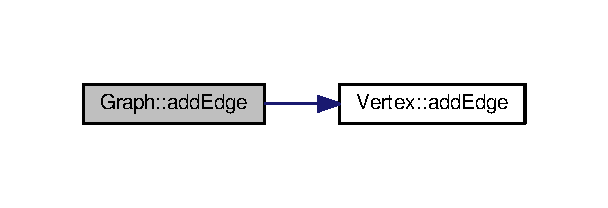
\includegraphics[width=292pt]{classGraph_afced43fb6c491d1294b00798dd9644ad_cgraph}
\end{center}
\end{figure}


\index{Graph@{Graph}!add\+Edge@{add\+Edge}}
\index{add\+Edge@{add\+Edge}!Graph@{Graph}}
\subsubsection[{\texorpdfstring{add\+Edge(const T \&edge\+Id, const string \&road\+Name, const T \&sourc, const T \&dest, int w, bool is\+Undirected)}{addEdge(const T &edgeId, const string &roadName, const T &sourc, const T &dest, int w, bool isUndirected)}}]{\setlength{\rightskip}{0pt plus 5cm}template$<$class T$>$ void {\bf Graph}$<$ T $>$\+::add\+Edge (
\begin{DoxyParamCaption}
\item[{const T \&}]{edge\+Id, }
\item[{const string \&}]{road\+Name, }
\item[{const T \&}]{sourc, }
\item[{const T \&}]{dest, }
\item[{int}]{w, }
\item[{bool}]{is\+Undirected}
\end{DoxyParamCaption}
)}\hypertarget{classGraph_af720eb3f731732a2fafc40141f4d41c3}{}\label{classGraph_af720eb3f731732a2fafc40141f4d41c3}


Here is the call graph for this function\+:
\nopagebreak
\begin{figure}[H]
\begin{center}
\leavevmode
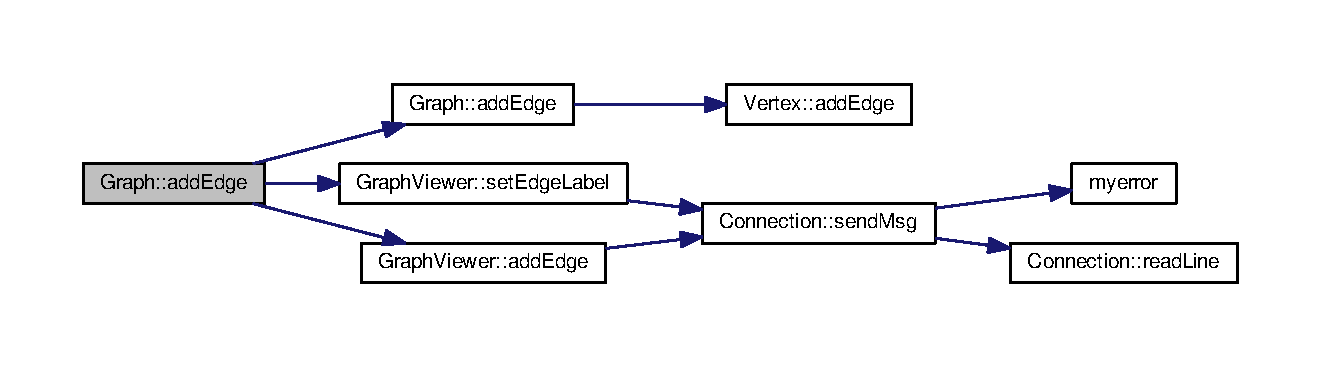
\includegraphics[width=350pt]{classGraph_af720eb3f731732a2fafc40141f4d41c3_cgraph}
\end{center}
\end{figure}


\index{Graph@{Graph}!add\+Vertex@{add\+Vertex}}
\index{add\+Vertex@{add\+Vertex}!Graph@{Graph}}
\subsubsection[{\texorpdfstring{add\+Vertex(const T \&in, std\+::pair$<$ double, double $>$ coords)}{addVertex(const T &in, std::pair< double, double > coords)}}]{\setlength{\rightskip}{0pt plus 5cm}template$<$class T$>$ bool {\bf Graph}$<$ T $>$\+::add\+Vertex (
\begin{DoxyParamCaption}
\item[{const T \&}]{in, }
\item[{std\+::pair$<$ double, double $>$}]{coords}
\end{DoxyParamCaption}
)}\hypertarget{classGraph_a18f099535183b37aef90bb55f4669e65}{}\label{classGraph_a18f099535183b37aef90bb55f4669e65}


Here is the call graph for this function\+:
\nopagebreak
\begin{figure}[H]
\begin{center}
\leavevmode
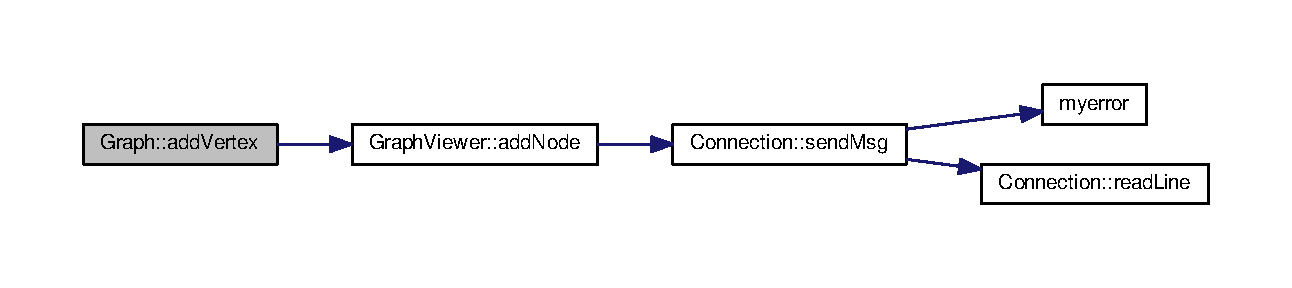
\includegraphics[width=350pt]{classGraph_a18f099535183b37aef90bb55f4669e65_cgraph}
\end{center}
\end{figure}


\index{Graph@{Graph}!bfs@{bfs}}
\index{bfs@{bfs}!Graph@{Graph}}
\subsubsection[{\texorpdfstring{bfs(\+Vertex$<$ T $>$ $\ast$v) const }{bfs(Vertex< T > *v) const }}]{\setlength{\rightskip}{0pt plus 5cm}template$<$class T$>$ vector$<$ T $>$ {\bf Graph}$<$ T $>$\+::bfs (
\begin{DoxyParamCaption}
\item[{{\bf Vertex}$<$ T $>$ $\ast$}]{v}
\end{DoxyParamCaption}
) const}\hypertarget{classGraph_a0e9598b98be2570eb432690411a577e8}{}\label{classGraph_a0e9598b98be2570eb432690411a577e8}


Here is the call graph for this function\+:
\nopagebreak
\begin{figure}[H]
\begin{center}
\leavevmode
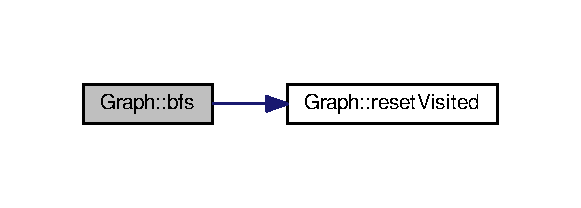
\includegraphics[width=279pt]{classGraph_a0e9598b98be2570eb432690411a577e8_cgraph}
\end{center}
\end{figure}


\index{Graph@{Graph}!dijkstra\+Shortest\+Path@{dijkstra\+Shortest\+Path}}
\index{dijkstra\+Shortest\+Path@{dijkstra\+Shortest\+Path}!Graph@{Graph}}
\subsubsection[{\texorpdfstring{dijkstra\+Shortest\+Path(const T \&s) const }{dijkstraShortestPath(const T &s) const }}]{\setlength{\rightskip}{0pt plus 5cm}template$<$class T$>$ void {\bf Graph}$<$ T $>$\+::dijkstra\+Shortest\+Path (
\begin{DoxyParamCaption}
\item[{const T \&}]{s}
\end{DoxyParamCaption}
) const}\hypertarget{classGraph_a3631bce147c033119e2d328848effd43}{}\label{classGraph_a3631bce147c033119e2d328848effd43}


Here is the call graph for this function\+:
\nopagebreak
\begin{figure}[H]
\begin{center}
\leavevmode
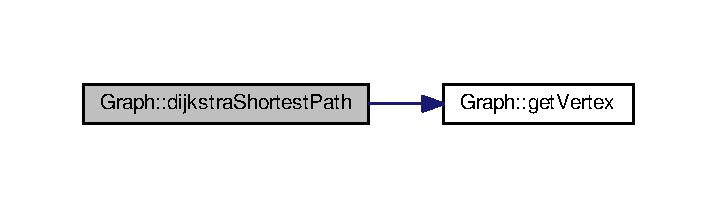
\includegraphics[width=344pt]{classGraph_a3631bce147c033119e2d328848effd43_cgraph}
\end{center}
\end{figure}


\index{Graph@{Graph}!edge\+Cost@{edge\+Cost}}
\index{edge\+Cost@{edge\+Cost}!Graph@{Graph}}
\subsubsection[{\texorpdfstring{edge\+Cost(int v\+Orig\+Index, int v\+Dest\+Index)}{edgeCost(int vOrigIndex, int vDestIndex)}}]{\setlength{\rightskip}{0pt plus 5cm}template$<$class T $>$ int {\bf Graph}$<$ T $>$\+::edge\+Cost (
\begin{DoxyParamCaption}
\item[{int}]{v\+Orig\+Index, }
\item[{int}]{v\+Dest\+Index}
\end{DoxyParamCaption}
)}\hypertarget{classGraph_a7e137f1ef838395ac1044a944fa54448}{}\label{classGraph_a7e137f1ef838395ac1044a944fa54448}
\index{Graph@{Graph}!floyd\+Warshall\+Shortest\+Path@{floyd\+Warshall\+Shortest\+Path}}
\index{floyd\+Warshall\+Shortest\+Path@{floyd\+Warshall\+Shortest\+Path}!Graph@{Graph}}
\subsubsection[{\texorpdfstring{floyd\+Warshall\+Shortest\+Path()}{floydWarshallShortestPath()}}]{\setlength{\rightskip}{0pt plus 5cm}template$<$class T $>$ void {\bf Graph}$<$ T $>$\+::floyd\+Warshall\+Shortest\+Path (
\begin{DoxyParamCaption}
{}
\end{DoxyParamCaption}
)}\hypertarget{classGraph_ae5161f4408bf1ead2b29d19d67fb04ee}{}\label{classGraph_ae5161f4408bf1ead2b29d19d67fb04ee}


Here is the call graph for this function\+:
\nopagebreak
\begin{figure}[H]
\begin{center}
\leavevmode
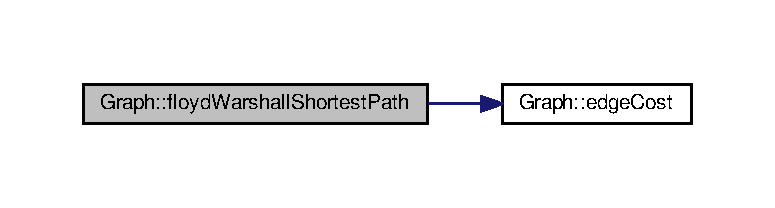
\includegraphics[width=350pt]{classGraph_ae5161f4408bf1ead2b29d19d67fb04ee_cgraph}
\end{center}
\end{figure}


\index{Graph@{Graph}!get\+Edge@{get\+Edge}}
\index{get\+Edge@{get\+Edge}!Graph@{Graph}}
\subsubsection[{\texorpdfstring{get\+Edge(const T \&v) const }{getEdge(const T &v) const }}]{\setlength{\rightskip}{0pt plus 5cm}template$<$class T$>$ {\bf Edge}$<$ T $>$ $\ast$ {\bf Graph}$<$ T $>$\+::get\+Edge (
\begin{DoxyParamCaption}
\item[{const T \&}]{v}
\end{DoxyParamCaption}
) const}\hypertarget{classGraph_af6579aaa220d1b403cb3517266e406cf}{}\label{classGraph_af6579aaa220d1b403cb3517266e406cf}
\index{Graph@{Graph}!get\+Edge@{get\+Edge}}
\index{get\+Edge@{get\+Edge}!Graph@{Graph}}
\subsubsection[{\texorpdfstring{get\+Edge(const T \&source, const T \&dest)}{getEdge(const T &source, const T &dest)}}]{\setlength{\rightskip}{0pt plus 5cm}template$<$class T$>$ int {\bf Graph}$<$ T $>$\+::get\+Edge (
\begin{DoxyParamCaption}
\item[{const T \&}]{source, }
\item[{const T \&}]{dest}
\end{DoxyParamCaption}
)}\hypertarget{classGraph_ac9ce9fbd0d125874296f2df5731e1a72}{}\label{classGraph_ac9ce9fbd0d125874296f2df5731e1a72}
\index{Graph@{Graph}!get\+Edges@{get\+Edges}}
\index{get\+Edges@{get\+Edges}!Graph@{Graph}}
\subsubsection[{\texorpdfstring{get\+Edges() const }{getEdges() const }}]{\setlength{\rightskip}{0pt plus 5cm}template$<$class T $>$ vector$<$ {\bf Edge}$<$ T $>$ $>$ {\bf Graph}$<$ T $>$\+::get\+Edges (
\begin{DoxyParamCaption}
{}
\end{DoxyParamCaption}
) const}\hypertarget{classGraph_aa46616d7684e3f3e69cb0d5497a8b45e}{}\label{classGraph_aa46616d7684e3f3e69cb0d5497a8b45e}
\index{Graph@{Graph}!getfloyd\+Warshall\+Path@{getfloyd\+Warshall\+Path}}
\index{getfloyd\+Warshall\+Path@{getfloyd\+Warshall\+Path}!Graph@{Graph}}
\subsubsection[{\texorpdfstring{getfloyd\+Warshall\+Path(const T \&origin, const T \&dest)}{getfloydWarshallPath(const T &origin, const T &dest)}}]{\setlength{\rightskip}{0pt plus 5cm}template$<$class T$>$ vector$<$ T $>$ {\bf Graph}$<$ T $>$\+::getfloyd\+Warshall\+Path (
\begin{DoxyParamCaption}
\item[{const T \&}]{origin, }
\item[{const T \&}]{dest}
\end{DoxyParamCaption}
)}\hypertarget{classGraph_ab23d1dae92a7f2b29dcb91a94336674c}{}\label{classGraph_ab23d1dae92a7f2b29dcb91a94336674c}


Here is the call graph for this function\+:
\nopagebreak
\begin{figure}[H]
\begin{center}
\leavevmode
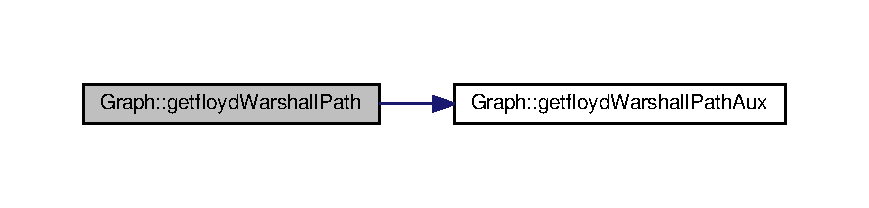
\includegraphics[width=350pt]{classGraph_ab23d1dae92a7f2b29dcb91a94336674c_cgraph}
\end{center}
\end{figure}


\index{Graph@{Graph}!getfloyd\+Warshall\+Path\+Aux@{getfloyd\+Warshall\+Path\+Aux}}
\index{getfloyd\+Warshall\+Path\+Aux@{getfloyd\+Warshall\+Path\+Aux}!Graph@{Graph}}
\subsubsection[{\texorpdfstring{getfloyd\+Warshall\+Path\+Aux(int index1, int index2, vector$<$ T $>$ \&res)}{getfloydWarshallPathAux(int index1, int index2, vector< T > &res)}}]{\setlength{\rightskip}{0pt plus 5cm}template$<$class T$>$ void {\bf Graph}$<$ T $>$\+::getfloyd\+Warshall\+Path\+Aux (
\begin{DoxyParamCaption}
\item[{int}]{index1, }
\item[{int}]{index2, }
\item[{vector$<$ T $>$ \&}]{res}
\end{DoxyParamCaption}
)}\hypertarget{classGraph_aad1eda4beb8425d03ed1f3b8af397563}{}\label{classGraph_aad1eda4beb8425d03ed1f3b8af397563}
\index{Graph@{Graph}!get\+GV@{get\+GV}}
\index{get\+GV@{get\+GV}!Graph@{Graph}}
\subsubsection[{\texorpdfstring{get\+G\+V() const }{getGV() const }}]{\setlength{\rightskip}{0pt plus 5cm}template$<$class T $>$ {\bf Graph\+Viewer} $\ast$ {\bf Graph}$<$ T $>$\+::get\+GV (
\begin{DoxyParamCaption}
{}
\end{DoxyParamCaption}
) const}\hypertarget{classGraph_a8cfc98c097359592094c27f2118dc6a7}{}\label{classGraph_a8cfc98c097359592094c27f2118dc6a7}
\index{Graph@{Graph}!get\+Num\+Edge@{get\+Num\+Edge}}
\index{get\+Num\+Edge@{get\+Num\+Edge}!Graph@{Graph}}
\subsubsection[{\texorpdfstring{get\+Num\+Edge() const }{getNumEdge() const }}]{\setlength{\rightskip}{0pt plus 5cm}template$<$class T $>$ int {\bf Graph}$<$ T $>$\+::get\+Num\+Edge (
\begin{DoxyParamCaption}
{}
\end{DoxyParamCaption}
) const}\hypertarget{classGraph_ad10eead5afadfb05a78fd8dd606238f8}{}\label{classGraph_ad10eead5afadfb05a78fd8dd606238f8}
\index{Graph@{Graph}!get\+Num\+Vertex@{get\+Num\+Vertex}}
\index{get\+Num\+Vertex@{get\+Num\+Vertex}!Graph@{Graph}}
\subsubsection[{\texorpdfstring{get\+Num\+Vertex() const }{getNumVertex() const }}]{\setlength{\rightskip}{0pt plus 5cm}template$<$class T $>$ int {\bf Graph}$<$ T $>$\+::get\+Num\+Vertex (
\begin{DoxyParamCaption}
{}
\end{DoxyParamCaption}
) const}\hypertarget{classGraph_a295932f117d92c825a97ec458e0fb332}{}\label{classGraph_a295932f117d92c825a97ec458e0fb332}
\index{Graph@{Graph}!get\+Path@{get\+Path}}
\index{get\+Path@{get\+Path}!Graph@{Graph}}
\subsubsection[{\texorpdfstring{get\+Path(const T \&origin, const T \&dest)}{getPath(const T &origin, const T &dest)}}]{\setlength{\rightskip}{0pt plus 5cm}template$<$class T$>$ vector$<$ T $>$ {\bf Graph}$<$ T $>$\+::get\+Path (
\begin{DoxyParamCaption}
\item[{const T \&}]{origin, }
\item[{const T \&}]{dest}
\end{DoxyParamCaption}
)}\hypertarget{classGraph_ab4054ca572c10669dd3e05d6d41c116c}{}\label{classGraph_ab4054ca572c10669dd3e05d6d41c116c}


Here is the call graph for this function\+:
\nopagebreak
\begin{figure}[H]
\begin{center}
\leavevmode
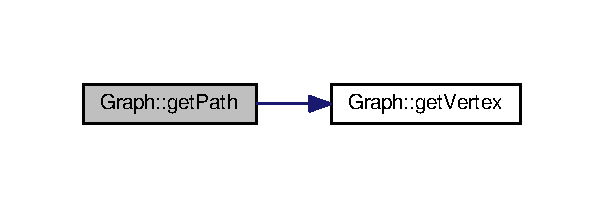
\includegraphics[width=290pt]{classGraph_ab4054ca572c10669dd3e05d6d41c116c_cgraph}
\end{center}
\end{figure}


\index{Graph@{Graph}!get\+Unique\+Edges@{get\+Unique\+Edges}}
\index{get\+Unique\+Edges@{get\+Unique\+Edges}!Graph@{Graph}}
\subsubsection[{\texorpdfstring{get\+Unique\+Edges()}{getUniqueEdges()}}]{\setlength{\rightskip}{0pt plus 5cm}template$<$class T $>$ vector$<$ int $>$ {\bf Graph}$<$ T $>$\+::get\+Unique\+Edges (
\begin{DoxyParamCaption}
{}
\end{DoxyParamCaption}
)}\hypertarget{classGraph_a6d54a3a7d9c687fa4d81af01c5ef5b75}{}\label{classGraph_a6d54a3a7d9c687fa4d81af01c5ef5b75}
\index{Graph@{Graph}!get\+Vertex@{get\+Vertex}}
\index{get\+Vertex@{get\+Vertex}!Graph@{Graph}}
\subsubsection[{\texorpdfstring{get\+Vertex(const T \&v) const }{getVertex(const T &v) const }}]{\setlength{\rightskip}{0pt plus 5cm}template$<$class T$>$ {\bf Vertex}$<$ T $>$ $\ast$ {\bf Graph}$<$ T $>$\+::get\+Vertex (
\begin{DoxyParamCaption}
\item[{const T \&}]{v}
\end{DoxyParamCaption}
) const}\hypertarget{classGraph_a08a95472b0d9bd7321660940807af060}{}\label{classGraph_a08a95472b0d9bd7321660940807af060}
\index{Graph@{Graph}!get\+Weight\+Floyd\+Warshall@{get\+Weight\+Floyd\+Warshall}}
\index{get\+Weight\+Floyd\+Warshall@{get\+Weight\+Floyd\+Warshall}!Graph@{Graph}}
\subsubsection[{\texorpdfstring{get\+Weight\+Floyd\+Warshall(int index1, int index2)}{getWeightFloydWarshall(int index1, int index2)}}]{\setlength{\rightskip}{0pt plus 5cm}template$<$class T $>$ int {\bf Graph}$<$ T $>$\+::get\+Weight\+Floyd\+Warshall (
\begin{DoxyParamCaption}
\item[{int}]{index1, }
\item[{int}]{index2}
\end{DoxyParamCaption}
)}\hypertarget{classGraph_ab314d60da32e5e0080e51c9c17f06f85}{}\label{classGraph_ab314d60da32e5e0080e51c9c17f06f85}
\index{Graph@{Graph}!reset\+Visited@{reset\+Visited}}
\index{reset\+Visited@{reset\+Visited}!Graph@{Graph}}
\subsubsection[{\texorpdfstring{reset\+Visited() const }{resetVisited() const }}]{\setlength{\rightskip}{0pt plus 5cm}template$<$class T $>$ void {\bf Graph}$<$ T $>$\+::reset\+Visited (
\begin{DoxyParamCaption}
{}
\end{DoxyParamCaption}
) const}\hypertarget{classGraph_a3c32b686c689011a360e7e25a76ee511}{}\label{classGraph_a3c32b686c689011a360e7e25a76ee511}


\subsection{Member Data Documentation}
\index{Graph@{Graph}!edges@{edges}}
\index{edges@{edges}!Graph@{Graph}}
\subsubsection[{\texorpdfstring{edges}{edges}}]{\setlength{\rightskip}{0pt plus 5cm}template$<$class T$>$ vector$<${\bf Edge}$<$T$>$ $>$ {\bf Graph}$<$ T $>$\+::edges\hspace{0.3cm}{\ttfamily [private]}}\hypertarget{classGraph_afbdd278e1f3cb43805ef769404a3afd1}{}\label{classGraph_afbdd278e1f3cb43805ef769404a3afd1}
\index{Graph@{Graph}!edge\+Set@{edge\+Set}}
\index{edge\+Set@{edge\+Set}!Graph@{Graph}}
\subsubsection[{\texorpdfstring{edge\+Set}{edgeSet}}]{\setlength{\rightskip}{0pt plus 5cm}template$<$class T$>$ vector$<${\bf Edge}$<$T$>$ $\ast$$>$ {\bf Graph}$<$ T $>$\+::edge\+Set\hspace{0.3cm}{\ttfamily [private]}}\hypertarget{classGraph_a83ebb4fdb2b6a21d4112d4d179230e95}{}\label{classGraph_a83ebb4fdb2b6a21d4112d4d179230e95}
\index{Graph@{Graph}!gv@{gv}}
\index{gv@{gv}!Graph@{Graph}}
\subsubsection[{\texorpdfstring{gv}{gv}}]{\setlength{\rightskip}{0pt plus 5cm}template$<$class T$>$ {\bf Graph\+Viewer}$\ast$ {\bf Graph}$<$ T $>$\+::gv\hspace{0.3cm}{\ttfamily [private]}}\hypertarget{classGraph_afbbcf226b738a3dd936173881991b31e}{}\label{classGraph_afbbcf226b738a3dd936173881991b31e}
\index{Graph@{Graph}!P@{P}}
\index{P@{P}!Graph@{Graph}}
\subsubsection[{\texorpdfstring{P}{P}}]{\setlength{\rightskip}{0pt plus 5cm}template$<$class T$>$ int$\ast$$\ast$ {\bf Graph}$<$ T $>$\+::P\hspace{0.3cm}{\ttfamily [private]}}\hypertarget{classGraph_a8198bca6e66c0c95e24062e40813ebba}{}\label{classGraph_a8198bca6e66c0c95e24062e40813ebba}
\index{Graph@{Graph}!unique\+Edges@{unique\+Edges}}
\index{unique\+Edges@{unique\+Edges}!Graph@{Graph}}
\subsubsection[{\texorpdfstring{unique\+Edges}{uniqueEdges}}]{\setlength{\rightskip}{0pt plus 5cm}template$<$class T$>$ vector$<$int$>$ {\bf Graph}$<$ T $>$\+::unique\+Edges\hspace{0.3cm}{\ttfamily [private]}}\hypertarget{classGraph_a6f829bb651ea6c0b2aa45564dd4eda25}{}\label{classGraph_a6f829bb651ea6c0b2aa45564dd4eda25}
\index{Graph@{Graph}!vertex\+Set@{vertex\+Set}}
\index{vertex\+Set@{vertex\+Set}!Graph@{Graph}}
\subsubsection[{\texorpdfstring{vertex\+Set}{vertexSet}}]{\setlength{\rightskip}{0pt plus 5cm}template$<$class T$>$ vector$<${\bf Vertex}$<$T$>$ $\ast$$>$ {\bf Graph}$<$ T $>$\+::vertex\+Set\hspace{0.3cm}{\ttfamily [private]}}\hypertarget{classGraph_a73d4e735fc0a7c83c9c689a2b53fa623}{}\label{classGraph_a73d4e735fc0a7c83c9c689a2b53fa623}
\index{Graph@{Graph}!W@{W}}
\index{W@{W}!Graph@{Graph}}
\subsubsection[{\texorpdfstring{W}{W}}]{\setlength{\rightskip}{0pt plus 5cm}template$<$class T$>$ int$\ast$$\ast$ {\bf Graph}$<$ T $>$\+::W\hspace{0.3cm}{\ttfamily [private]}}\hypertarget{classGraph_a20edce9af2c8ea8725ccbb5201eace38}{}\label{classGraph_a20edce9af2c8ea8725ccbb5201eace38}


The documentation for this class was generated from the following file\+:\begin{DoxyCompactItemize}
\item 
/home/ana/\+Dropbox/faculdade/2ano/2semestre/\+C\+A\+L/\+Smart\+Waste/src/\hyperlink{Graph_8h}{Graph.\+h}\end{DoxyCompactItemize}

\hypertarget{classGraphViewer}{}\section{Graph\+Viewer Class Reference}
\label{classGraphViewer}\index{Graph\+Viewer@{Graph\+Viewer}}


{\ttfamily \#include $<$graphviewer.\+h$>$}



Collaboration diagram for Graph\+Viewer\+:
\nopagebreak
\begin{figure}[H]
\begin{center}
\leavevmode
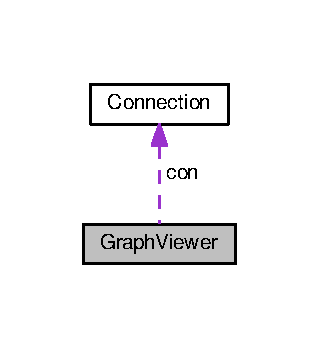
\includegraphics[width=153pt]{classGraphViewer__coll__graph}
\end{center}
\end{figure}
\subsection*{Public Member Functions}
\begin{DoxyCompactItemize}
\item 
\hyperlink{classGraphViewer_a8adc614f4fc290a3efcec7d7ceb1c58a}{Graph\+Viewer} (int \hyperlink{classGraphViewer_a5de27a1d20968b8494cd4bf5a4eb27e1}{width}, int \hyperlink{classGraphViewer_a9a1000e492a66ac4301c7135275690da}{height}, bool dynamic)
\item 
\hyperlink{classGraphViewer_ad9d7b1d8b4ba8ef18517eae0e68568a2}{Graph\+Viewer} (int \hyperlink{classGraphViewer_a5de27a1d20968b8494cd4bf5a4eb27e1}{width}, int \hyperlink{classGraphViewer_a9a1000e492a66ac4301c7135275690da}{height}, bool dynamic, int port\+\_\+n)
\item 
bool \hyperlink{classGraphViewer_ae5247dc66449dcd21fc5d531bbbaddfa}{create\+Window} (int \hyperlink{classGraphViewer_a5de27a1d20968b8494cd4bf5a4eb27e1}{width}, int \hyperlink{classGraphViewer_a9a1000e492a66ac4301c7135275690da}{height})
\item 
bool \hyperlink{classGraphViewer_a85990c1eaac7feed3950960d4bd2fd4c}{close\+Window} ()
\item 
bool \hyperlink{classGraphViewer_a5421e86ac76433876309236ba96e70a2}{add\+Node} (int id, int x, int y)
\item 
bool \hyperlink{classGraphViewer_ab9be856eb5f45284719a3bb119ec01ea}{add\+Node} (int id)
\item 
bool \hyperlink{classGraphViewer_aad0c1448c37f744209ffb671f1bd0015}{add\+Edge} (int id, int v1, int v2, int edge\+Type)
\item 
bool \hyperlink{classGraphViewer_a0c418639bb911eb827cabf895915f775}{remove\+Node} (int id)
\item 
bool \hyperlink{classGraphViewer_a9a8ee68c7c12b373affbe4069dd95d72}{remove\+Edge} (int id)
\item 
bool \hyperlink{classGraphViewer_ac25d7d007022fda16799808ba136e909}{set\+Vertex\+Label} (int id, string label)
\item 
bool \hyperlink{classGraphViewer_a007bd78a6959ac37119eb18a8e8bca4c}{clear\+Vertex\+Label} (int id)
\item 
bool \hyperlink{classGraphViewer_a447cca0064e785654c2105602c2961ca}{set\+Edge\+Label} (int id, string label)
\item 
bool \hyperlink{classGraphViewer_a8b90527371bd990806eb32620be765be}{clear\+Edge\+Label} (int id)
\item 
bool \hyperlink{classGraphViewer_a07ccc96707efae4aa5f3ced3dca015af}{set\+Edge\+Color} (int id, string color)
\item 
bool \hyperlink{classGraphViewer_a0e3bb8f6d7290e141c141ca83c9eb67a}{clear\+Edge\+Color} (int id)
\item 
bool \hyperlink{classGraphViewer_a1698f1c6b3a8e7cabc7b7d7cf42fc7f0}{set\+Edge\+Dashed} (int id, bool dashed)
\item 
bool \hyperlink{classGraphViewer_a8b542d7e09e81a45a74760c19233beb0}{set\+Vertex\+Color} (int id, string color)
\item 
bool \hyperlink{classGraphViewer_a70e2f6cc24e545a66312a92cf5839d25}{clear\+Vertex\+Color} (int id)
\item 
bool \hyperlink{classGraphViewer_ae930dfdfcdeb7a871eefb6028d74b9f9}{set\+Vertex\+Size} (int id, int size)
\item 
bool \hyperlink{classGraphViewer_a02d5f7393eab9a2d1b66719039597a64}{set\+Vertex\+Icon} (int id, string filepath)
\item 
bool \hyperlink{classGraphViewer_aecbeec01205b7f93cf73a65282f2daba}{clear\+Vertex\+Icon} (int id)
\item 
bool \hyperlink{classGraphViewer_a07f598272fe3515455eab13be749604a}{set\+Edge\+Thickness} (int id, int thickness)
\item 
bool \hyperlink{classGraphViewer_ac211de009a0afe2e6d44f4f8d030a2cc}{set\+Edge\+Weight} (int id, int weight)
\item 
bool \hyperlink{classGraphViewer_a69eb065145063e4dea41961e92e35c8e}{set\+Edge\+Flow} (int id, int flow)
\item 
bool \hyperlink{classGraphViewer_a08f362be0e682d91e7506dca8caae1b8}{define\+Edge\+Curved} (bool curved)
\item 
bool \hyperlink{classGraphViewer_a4102580b69826ba83251ef7bb262f8be}{define\+Edge\+Color} (string color)
\item 
bool \hyperlink{classGraphViewer_a1df1a30f4668bf70364fac232f8d0600}{reset\+Edge\+Color} ()
\item 
bool \hyperlink{classGraphViewer_af785279b5c204df0e274b20c36276fc3}{define\+Edge\+Dashed} (bool dashed)
\item 
bool \hyperlink{classGraphViewer_a76de8676b7a93d72af514b84cdaa4d21}{define\+Vertex\+Color} (string color)
\item 
bool \hyperlink{classGraphViewer_acd95eee309d5e9b1935ec39c5ed45cac}{reset\+Vertex\+Color} ()
\item 
bool \hyperlink{classGraphViewer_ac4b2a9fec74d38e64088aa79ca4b7d9b}{define\+Vertex\+Size} (int size)
\item 
bool \hyperlink{classGraphViewer_af1adb6a361457187a820e01dcf0a34b7}{define\+Vertex\+Icon} (string filepath)
\item 
bool \hyperlink{classGraphViewer_ae2b602cfdfb49ec0a67f2bcd11b0fbdb}{reset\+Vertex\+Icon} ()
\item 
bool \hyperlink{classGraphViewer_a02437b5fecd8b90de24436068312d593}{set\+Background} (string path)
\item 
bool \hyperlink{classGraphViewer_a5a03467a98312f2fef5b337677b104a8}{clear\+Background} ()
\item 
bool \hyperlink{classGraphViewer_a3009a66958686ccb7e78b68e37c3c423}{rearrange} ()
\end{DoxyCompactItemize}
\subsection*{Static Public Attributes}
\begin{DoxyCompactItemize}
\item 
static short \hyperlink{classGraphViewer_a89d0abe75f41feededc49497cc514342}{port} = 7772
\end{DoxyCompactItemize}
\subsection*{Private Member Functions}
\begin{DoxyCompactItemize}
\item 
void \hyperlink{classGraphViewer_a1ce9dff4903c650d3b2d33a3ef1d1f61}{initialize} (int, int, bool, int)
\end{DoxyCompactItemize}
\subsection*{Private Attributes}
\begin{DoxyCompactItemize}
\item 
int \hyperlink{classGraphViewer_a5de27a1d20968b8494cd4bf5a4eb27e1}{width}
\item 
int \hyperlink{classGraphViewer_a9a1000e492a66ac4301c7135275690da}{height}
\item 
bool \hyperlink{classGraphViewer_a9d9947154bc63354c6d02a0680aad952}{is\+Dynamic}
\item 
\hyperlink{classConnection}{Connection} $\ast$ \hyperlink{classGraphViewer_a14a206f78c242e739e0908b06070ba4d}{con}
\end{DoxyCompactItemize}


\subsection{Detailed Description}
Classe que guarda o grafo e o representa. Todas as suas funções retornam um booleano a indicar se a sua execução decorreu ou não com sucesso. 

\subsection{Constructor \& Destructor Documentation}
\index{Graph\+Viewer@{Graph\+Viewer}!Graph\+Viewer@{Graph\+Viewer}}
\index{Graph\+Viewer@{Graph\+Viewer}!Graph\+Viewer@{Graph\+Viewer}}
\subsubsection[{\texorpdfstring{Graph\+Viewer(int width, int height, bool dynamic)}{GraphViewer(int width, int height, bool dynamic)}}]{\setlength{\rightskip}{0pt plus 5cm}Graph\+Viewer\+::\+Graph\+Viewer (
\begin{DoxyParamCaption}
\item[{int}]{width, }
\item[{int}]{height, }
\item[{bool}]{dynamic}
\end{DoxyParamCaption}
)}\hypertarget{classGraphViewer_a8adc614f4fc290a3efcec7d7ceb1c58a}{}\label{classGraphViewer_a8adc614f4fc290a3efcec7d7ceb1c58a}
Construtor que cria um novo grafo e atribui automaticamente a porta. Exemplo\+: \hyperlink{classGraphViewer}{Graph\+Viewer} $\ast$gv = new \hyperlink{classGraphViewer}{Graph\+Viewer(600, 600, true)}; instancia um grafo 600x600, onde a posição dos nós é determinada automaticamente.


\begin{DoxyParams}{Parameters}
{\em width} & Inteiro que representa a lagura da área do grafo. \\
\hline
{\em height} & Inteiro que representa a altura da área do grafo. \\
\hline
{\em dynamic} & Booleano que determina se a localização dos nós é automaticamente. determinado pelo programa (true) ou se deve ser determinado pelo utilizador (false). \\
\hline
\end{DoxyParams}


Here is the call graph for this function\+:
\nopagebreak
\begin{figure}[H]
\begin{center}
\leavevmode
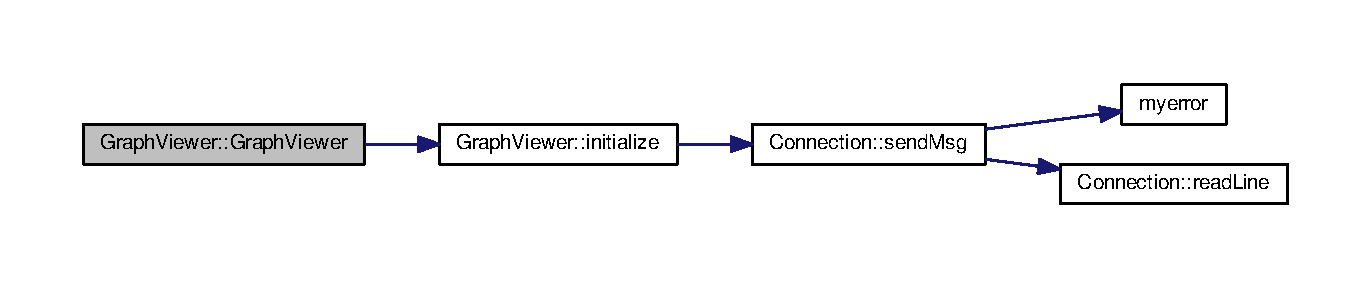
\includegraphics[width=350pt]{classGraphViewer_a8adc614f4fc290a3efcec7d7ceb1c58a_cgraph}
\end{center}
\end{figure}


\index{Graph\+Viewer@{Graph\+Viewer}!Graph\+Viewer@{Graph\+Viewer}}
\index{Graph\+Viewer@{Graph\+Viewer}!Graph\+Viewer@{Graph\+Viewer}}
\subsubsection[{\texorpdfstring{Graph\+Viewer(int width, int height, bool dynamic, int port\+\_\+n)}{GraphViewer(int width, int height, bool dynamic, int port_n)}}]{\setlength{\rightskip}{0pt plus 5cm}Graph\+Viewer\+::\+Graph\+Viewer (
\begin{DoxyParamCaption}
\item[{int}]{width, }
\item[{int}]{height, }
\item[{bool}]{dynamic, }
\item[{int}]{port\+\_\+n}
\end{DoxyParamCaption}
)}\hypertarget{classGraphViewer_ad9d7b1d8b4ba8ef18517eae0e68568a2}{}\label{classGraphViewer_ad9d7b1d8b4ba8ef18517eae0e68568a2}
Construtor que cria um novo grafo, utilizando uma porta especificada pelo utilizador para a ligação.

Exemplo\+: \hyperlink{classGraphViewer}{Graph\+Viewer} $\ast$gv = new \hyperlink{classGraphViewer}{Graph\+Viewer(600, 600, false, 3000)}; instancia um grafo 600x600, onde a posição dos nós é determinada pelo utilizador (usando a versão de add\+Node onde se pode especificar as coordenadas), sendo que a porta a usar para a comunicação é a 3000.


\begin{DoxyParams}{Parameters}
{\em width} & Inteiro que representa a lagura da área do grafo. \\
\hline
{\em height} & Inteiro que representa a altura da área do grafo. \\
\hline
{\em dynamic} & Booleano que determina se a localização dos nós é automaticamente. determinado pelo programa (true) ou se deve ser determinado pelo utilizador (false). \\
\hline
{\em port\+\_\+n} & Inteiro que determina a porta a utilizar. Deve-\/se ter cuidado para não utilizar uma porta já usada por outro programa ou pelo sistema. \\
\hline
\end{DoxyParams}


Here is the call graph for this function\+:
\nopagebreak
\begin{figure}[H]
\begin{center}
\leavevmode
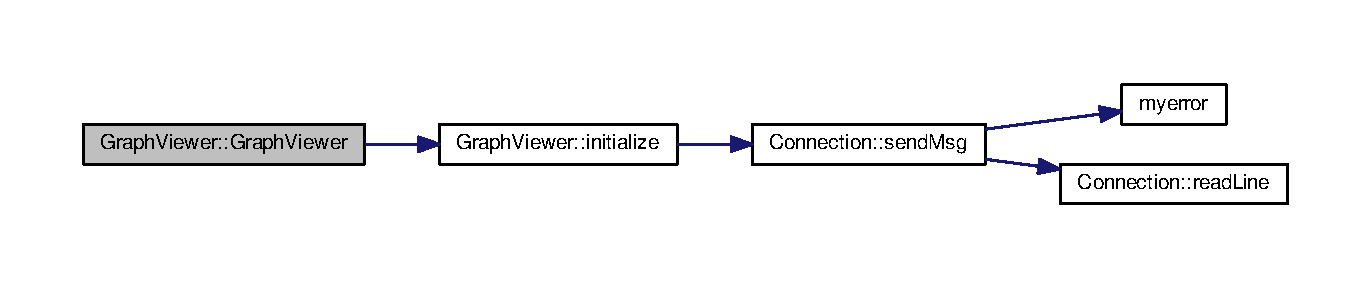
\includegraphics[width=350pt]{classGraphViewer_ad9d7b1d8b4ba8ef18517eae0e68568a2_cgraph}
\end{center}
\end{figure}




\subsection{Member Function Documentation}
\index{Graph\+Viewer@{Graph\+Viewer}!add\+Edge@{add\+Edge}}
\index{add\+Edge@{add\+Edge}!Graph\+Viewer@{Graph\+Viewer}}
\subsubsection[{\texorpdfstring{add\+Edge(int id, int v1, int v2, int edge\+Type)}{addEdge(int id, int v1, int v2, int edgeType)}}]{\setlength{\rightskip}{0pt plus 5cm}bool Graph\+Viewer\+::add\+Edge (
\begin{DoxyParamCaption}
\item[{int}]{id, }
\item[{int}]{v1, }
\item[{int}]{v2, }
\item[{int}]{edge\+Type}
\end{DoxyParamCaption}
)}\hypertarget{classGraphViewer_aad0c1448c37f744209ffb671f1bd0015}{}\label{classGraphViewer_aad0c1448c37f744209ffb671f1bd0015}
Acrescenta uma aresta à representação do grafo. Exemplo, para um apontador gv onde foi instanciada a classe \hyperlink{classGraphViewer}{Graph\+Viewer}\+: gv-\/$>$add\+Edge(0, 1, 2, Edge\+Type\+::\+U\+N\+D\+I\+R\+E\+C\+T\+E\+D); adiciona uma aresta não-\/dirigida com ID 0 que liga os nós com os I\+Ds 1 e 2


\begin{DoxyParams}{Parameters}
{\em id} & Identificador único da aresta. \\
\hline
{\em v1} & Identificador único do nó de origem da aresta. \\
\hline
{\em v2} & Identificador único do nó de destino da aresta. \\
\hline
{\em edge\+Type} & \hyperlink{classEdgeType_a903017a534f2818c2d17145e4ae0321c}{Edge\+Type.\+D\+I\+R\+E\+C\+T\+ED} caso a aresta seja unidirecional ou \hyperlink{classEdgeType_a6533cc56d05c288a550b9980b66c9317}{Edge\+Type.\+U\+N\+D\+I\+R\+E\+C\+T\+ED} caso a aresta seja bidirecional. \\
\hline
\end{DoxyParams}


Here is the call graph for this function\+:
\nopagebreak
\begin{figure}[H]
\begin{center}
\leavevmode
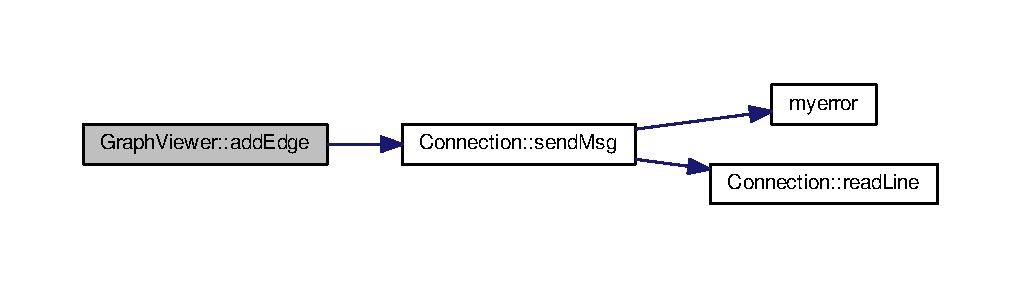
\includegraphics[width=350pt]{classGraphViewer_aad0c1448c37f744209ffb671f1bd0015_cgraph}
\end{center}
\end{figure}


\index{Graph\+Viewer@{Graph\+Viewer}!add\+Node@{add\+Node}}
\index{add\+Node@{add\+Node}!Graph\+Viewer@{Graph\+Viewer}}
\subsubsection[{\texorpdfstring{add\+Node(int id, int x, int y)}{addNode(int id, int x, int y)}}]{\setlength{\rightskip}{0pt plus 5cm}bool Graph\+Viewer\+::add\+Node (
\begin{DoxyParamCaption}
\item[{int}]{id, }
\item[{int}]{x, }
\item[{int}]{y}
\end{DoxyParamCaption}
)}\hypertarget{classGraphViewer_a5421e86ac76433876309236ba96e70a2}{}\label{classGraphViewer_a5421e86ac76433876309236ba96e70a2}
Acrescenta um nó à representação do grafo, numa posição específica, irrelevante se o grafo for dinâmico. Exemplo, para um apontador gv onde foi instanciada a classe \hyperlink{classGraphViewer}{Graph\+Viewer} com is\+Dynamic = false\+: gv-\/$>$add\+Node(0, 1, 2); adiciona um nó com ID 0 na posição (x, y) = (1, 2)


\begin{DoxyParams}{Parameters}
{\em id} & Identificador único do nó. \\
\hline
{\em x} & Posição horizontal do nó. \\
\hline
{\em y} & Posição vertical do nó. \\
\hline
\end{DoxyParams}


Here is the call graph for this function\+:
\nopagebreak
\begin{figure}[H]
\begin{center}
\leavevmode
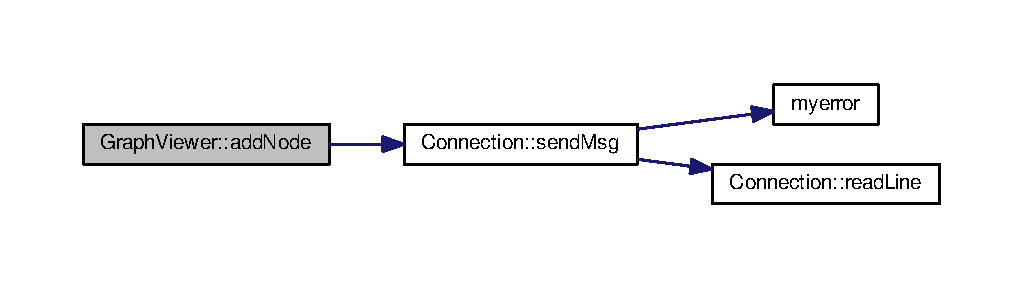
\includegraphics[width=350pt]{classGraphViewer_a5421e86ac76433876309236ba96e70a2_cgraph}
\end{center}
\end{figure}


\index{Graph\+Viewer@{Graph\+Viewer}!add\+Node@{add\+Node}}
\index{add\+Node@{add\+Node}!Graph\+Viewer@{Graph\+Viewer}}
\subsubsection[{\texorpdfstring{add\+Node(int id)}{addNode(int id)}}]{\setlength{\rightskip}{0pt plus 5cm}bool Graph\+Viewer\+::add\+Node (
\begin{DoxyParamCaption}
\item[{int}]{id}
\end{DoxyParamCaption}
)}\hypertarget{classGraphViewer_ab9be856eb5f45284719a3bb119ec01ea}{}\label{classGraphViewer_ab9be856eb5f45284719a3bb119ec01ea}
Acrescenta um nó à representação do grafo, numa posição ao critério do programa. Só pode ser usado se o grafo for dinâmico, ou seja, se as posições de todos os nós forem atribuídas automaticamente. Caso contrário, não adiciona o nó. Exemplo, para um apontador gv onde foi instanciada a classe \hyperlink{classGraphViewer}{Graph\+Viewer} com is\+Dynamic = true\+: gv-\/$>$add\+Node(0); adiciona um nó com ID 0


\begin{DoxyParams}{Parameters}
{\em id} & Identificador único do nó. \\
\hline
\end{DoxyParams}


Here is the call graph for this function\+:
\nopagebreak
\begin{figure}[H]
\begin{center}
\leavevmode
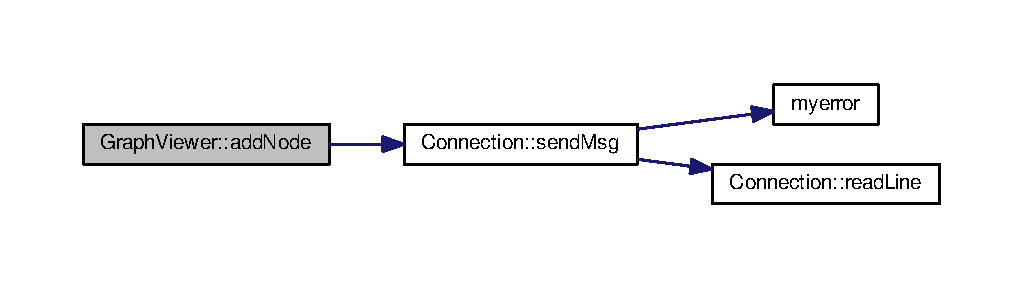
\includegraphics[width=350pt]{classGraphViewer_ab9be856eb5f45284719a3bb119ec01ea_cgraph}
\end{center}
\end{figure}


\index{Graph\+Viewer@{Graph\+Viewer}!clear\+Background@{clear\+Background}}
\index{clear\+Background@{clear\+Background}!Graph\+Viewer@{Graph\+Viewer}}
\subsubsection[{\texorpdfstring{clear\+Background()}{clearBackground()}}]{\setlength{\rightskip}{0pt plus 5cm}bool Graph\+Viewer\+::clear\+Background (
\begin{DoxyParamCaption}
{}
\end{DoxyParamCaption}
)}\hypertarget{classGraphViewer_a5a03467a98312f2fef5b337677b104a8}{}\label{classGraphViewer_a5a03467a98312f2fef5b337677b104a8}
Apaga a imagem de fundo do grafo, se tiver sido previamente definida. 

Here is the call graph for this function\+:
\nopagebreak
\begin{figure}[H]
\begin{center}
\leavevmode
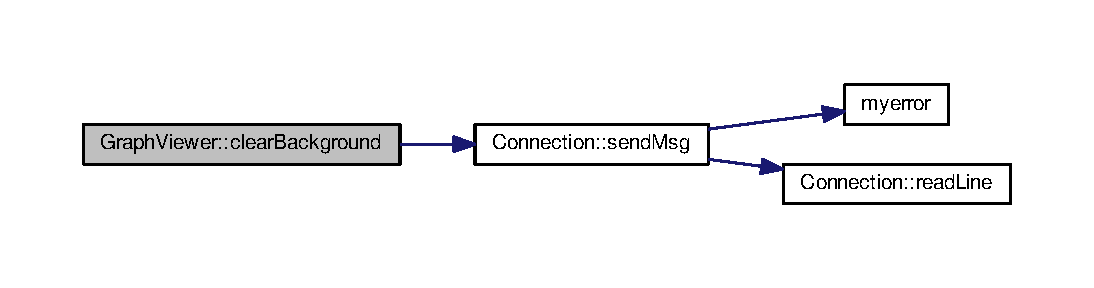
\includegraphics[width=350pt]{classGraphViewer_a5a03467a98312f2fef5b337677b104a8_cgraph}
\end{center}
\end{figure}


\index{Graph\+Viewer@{Graph\+Viewer}!clear\+Edge\+Color@{clear\+Edge\+Color}}
\index{clear\+Edge\+Color@{clear\+Edge\+Color}!Graph\+Viewer@{Graph\+Viewer}}
\subsubsection[{\texorpdfstring{clear\+Edge\+Color(int id)}{clearEdgeColor(int id)}}]{\setlength{\rightskip}{0pt plus 5cm}bool Graph\+Viewer\+::clear\+Edge\+Color (
\begin{DoxyParamCaption}
\item[{int}]{id}
\end{DoxyParamCaption}
)}\hypertarget{classGraphViewer_a0e3bb8f6d7290e141c141ca83c9eb67a}{}\label{classGraphViewer_a0e3bb8f6d7290e141c141ca83c9eb67a}
Função que apaga a cor de uma aresta, caso tenha sido definida.


\begin{DoxyParams}{Parameters}
{\em id} & Identificador único da aresta com a cor a apagar. \\
\hline
\end{DoxyParams}


Here is the call graph for this function\+:
\nopagebreak
\begin{figure}[H]
\begin{center}
\leavevmode
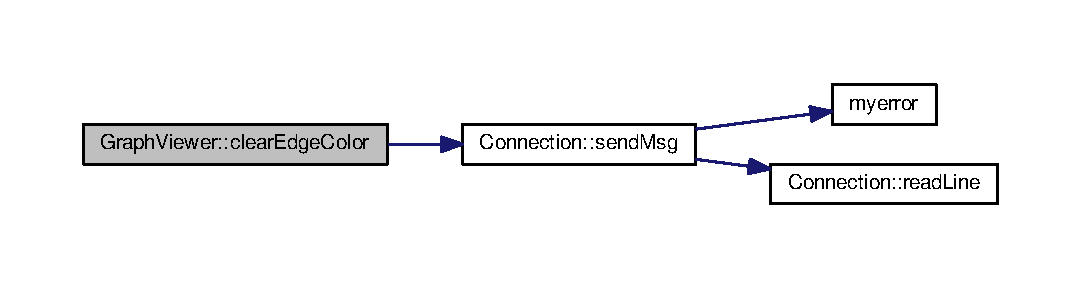
\includegraphics[width=350pt]{classGraphViewer_a0e3bb8f6d7290e141c141ca83c9eb67a_cgraph}
\end{center}
\end{figure}


\index{Graph\+Viewer@{Graph\+Viewer}!clear\+Edge\+Label@{clear\+Edge\+Label}}
\index{clear\+Edge\+Label@{clear\+Edge\+Label}!Graph\+Viewer@{Graph\+Viewer}}
\subsubsection[{\texorpdfstring{clear\+Edge\+Label(int id)}{clearEdgeLabel(int id)}}]{\setlength{\rightskip}{0pt plus 5cm}bool Graph\+Viewer\+::clear\+Edge\+Label (
\begin{DoxyParamCaption}
\item[{int}]{id}
\end{DoxyParamCaption}
)}\hypertarget{classGraphViewer_a8b90527371bd990806eb32620be765be}{}\label{classGraphViewer_a8b90527371bd990806eb32620be765be}
Função que apaga o texto de uma aresta, caso o mesmo tenha sido definido anteriormente.


\begin{DoxyParams}{Parameters}
{\em id} & Identificador único da aresta com o texto a apagar. \\
\hline
\end{DoxyParams}


Here is the call graph for this function\+:
\nopagebreak
\begin{figure}[H]
\begin{center}
\leavevmode
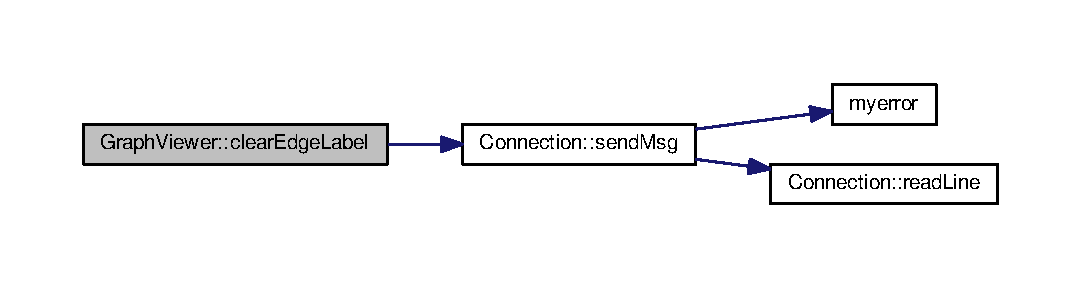
\includegraphics[width=350pt]{classGraphViewer_a8b90527371bd990806eb32620be765be_cgraph}
\end{center}
\end{figure}


\index{Graph\+Viewer@{Graph\+Viewer}!clear\+Vertex\+Color@{clear\+Vertex\+Color}}
\index{clear\+Vertex\+Color@{clear\+Vertex\+Color}!Graph\+Viewer@{Graph\+Viewer}}
\subsubsection[{\texorpdfstring{clear\+Vertex\+Color(int id)}{clearVertexColor(int id)}}]{\setlength{\rightskip}{0pt plus 5cm}bool Graph\+Viewer\+::clear\+Vertex\+Color (
\begin{DoxyParamCaption}
\item[{int}]{id}
\end{DoxyParamCaption}
)}\hypertarget{classGraphViewer_a70e2f6cc24e545a66312a92cf5839d25}{}\label{classGraphViewer_a70e2f6cc24e545a66312a92cf5839d25}
Função que apaga a cor de um vértice, colocando-\/a com o valor por omissão.


\begin{DoxyParams}{Parameters}
{\em id} & Identificador único do nó com a cor a apagar. \\
\hline
\end{DoxyParams}


Here is the call graph for this function\+:
\nopagebreak
\begin{figure}[H]
\begin{center}
\leavevmode
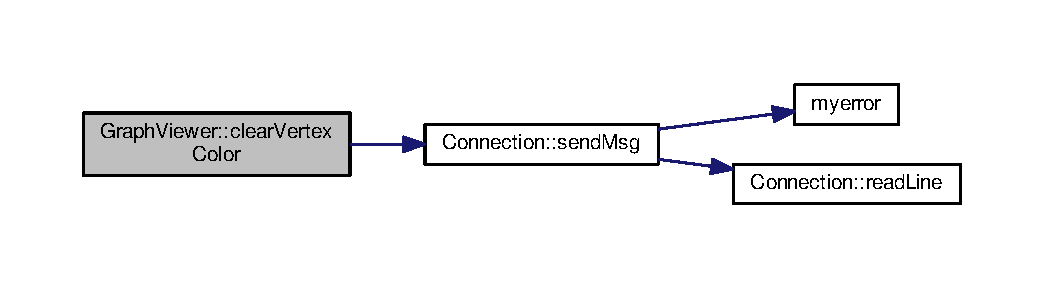
\includegraphics[width=350pt]{classGraphViewer_a70e2f6cc24e545a66312a92cf5839d25_cgraph}
\end{center}
\end{figure}


\index{Graph\+Viewer@{Graph\+Viewer}!clear\+Vertex\+Icon@{clear\+Vertex\+Icon}}
\index{clear\+Vertex\+Icon@{clear\+Vertex\+Icon}!Graph\+Viewer@{Graph\+Viewer}}
\subsubsection[{\texorpdfstring{clear\+Vertex\+Icon(int id)}{clearVertexIcon(int id)}}]{\setlength{\rightskip}{0pt plus 5cm}bool Graph\+Viewer\+::clear\+Vertex\+Icon (
\begin{DoxyParamCaption}
\item[{int}]{id}
\end{DoxyParamCaption}
)}\hypertarget{classGraphViewer_aecbeec01205b7f93cf73a65282f2daba}{}\label{classGraphViewer_aecbeec01205b7f93cf73a65282f2daba}
Função que apaga o ícone de um nó, caso tenha sido definido.


\begin{DoxyParams}{Parameters}
{\em id} & Identificador único do nó com o ícone a apagar. \\
\hline
\end{DoxyParams}


Here is the call graph for this function\+:
\nopagebreak
\begin{figure}[H]
\begin{center}
\leavevmode
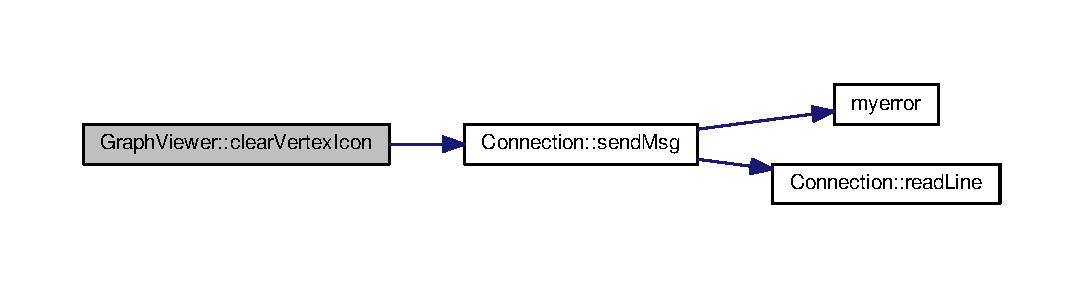
\includegraphics[width=350pt]{classGraphViewer_aecbeec01205b7f93cf73a65282f2daba_cgraph}
\end{center}
\end{figure}


\index{Graph\+Viewer@{Graph\+Viewer}!clear\+Vertex\+Label@{clear\+Vertex\+Label}}
\index{clear\+Vertex\+Label@{clear\+Vertex\+Label}!Graph\+Viewer@{Graph\+Viewer}}
\subsubsection[{\texorpdfstring{clear\+Vertex\+Label(int id)}{clearVertexLabel(int id)}}]{\setlength{\rightskip}{0pt plus 5cm}bool Graph\+Viewer\+::clear\+Vertex\+Label (
\begin{DoxyParamCaption}
\item[{int}]{id}
\end{DoxyParamCaption}
)}\hypertarget{classGraphViewer_a007bd78a6959ac37119eb18a8e8bca4c}{}\label{classGraphViewer_a007bd78a6959ac37119eb18a8e8bca4c}
Função que apaga o texto de um nó, caso o mesmo tenha sido definido anteriormente.


\begin{DoxyParams}{Parameters}
{\em id} & Identificador único do nó com o texto a apagar. \\
\hline
\end{DoxyParams}


Here is the call graph for this function\+:
\nopagebreak
\begin{figure}[H]
\begin{center}
\leavevmode
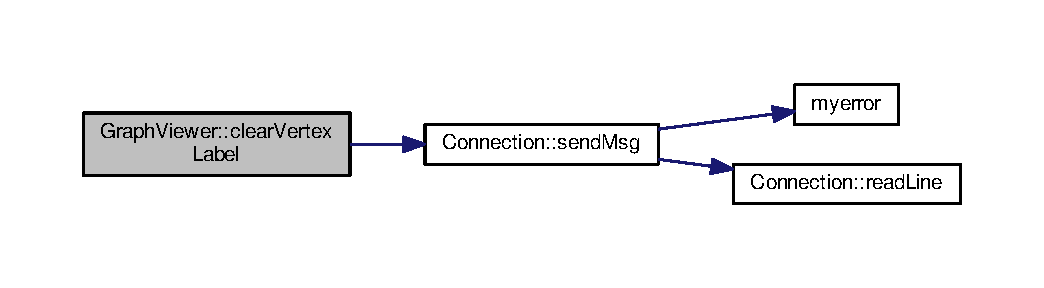
\includegraphics[width=350pt]{classGraphViewer_a007bd78a6959ac37119eb18a8e8bca4c_cgraph}
\end{center}
\end{figure}


\index{Graph\+Viewer@{Graph\+Viewer}!close\+Window@{close\+Window}}
\index{close\+Window@{close\+Window}!Graph\+Viewer@{Graph\+Viewer}}
\subsubsection[{\texorpdfstring{close\+Window()}{closeWindow()}}]{\setlength{\rightskip}{0pt plus 5cm}bool Graph\+Viewer\+::close\+Window (
\begin{DoxyParamCaption}
{}
\end{DoxyParamCaption}
)}\hypertarget{classGraphViewer_a85990c1eaac7feed3950960d4bd2fd4c}{}\label{classGraphViewer_a85990c1eaac7feed3950960d4bd2fd4c}
Fecha a janela a ser utilizada para visualização. 

Here is the call graph for this function\+:
\nopagebreak
\begin{figure}[H]
\begin{center}
\leavevmode
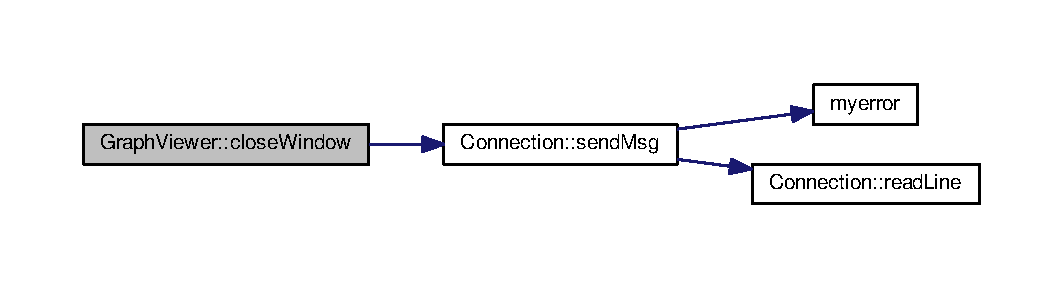
\includegraphics[width=350pt]{classGraphViewer_a85990c1eaac7feed3950960d4bd2fd4c_cgraph}
\end{center}
\end{figure}


\index{Graph\+Viewer@{Graph\+Viewer}!create\+Window@{create\+Window}}
\index{create\+Window@{create\+Window}!Graph\+Viewer@{Graph\+Viewer}}
\subsubsection[{\texorpdfstring{create\+Window(int width, int height)}{createWindow(int width, int height)}}]{\setlength{\rightskip}{0pt plus 5cm}bool Graph\+Viewer\+::create\+Window (
\begin{DoxyParamCaption}
\item[{int}]{width, }
\item[{int}]{height}
\end{DoxyParamCaption}
)}\hypertarget{classGraphViewer_ae5247dc66449dcd21fc5d531bbbaddfa}{}\label{classGraphViewer_ae5247dc66449dcd21fc5d531bbbaddfa}
Função que cria a janela para visualização. Exemplo, para um apontador gv onde foi instanciada a classe \hyperlink{classGraphViewer}{Graph\+Viewer}\+: gv-\/$>$create\+Window(600, 600); abre uma janela 600x600 onde mostra o grafo.


\begin{DoxyParams}{Parameters}
{\em width} & Largura da janela a criar. \\
\hline
{\em height} & Altura da janela a criar. \\
\hline
\end{DoxyParams}


Here is the call graph for this function\+:
\nopagebreak
\begin{figure}[H]
\begin{center}
\leavevmode
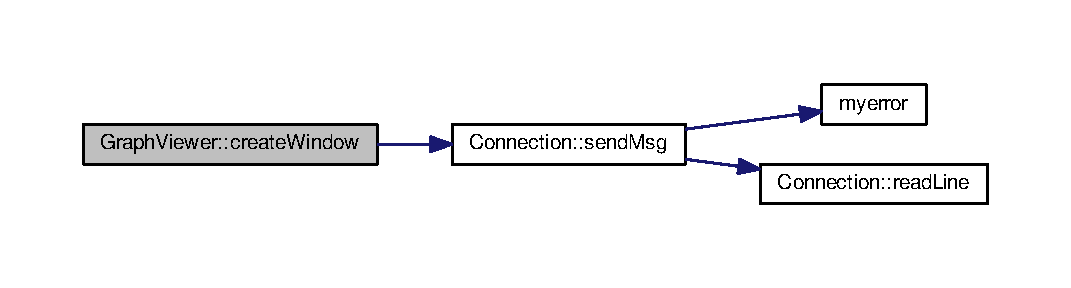
\includegraphics[width=350pt]{classGraphViewer_ae5247dc66449dcd21fc5d531bbbaddfa_cgraph}
\end{center}
\end{figure}


\index{Graph\+Viewer@{Graph\+Viewer}!define\+Edge\+Color@{define\+Edge\+Color}}
\index{define\+Edge\+Color@{define\+Edge\+Color}!Graph\+Viewer@{Graph\+Viewer}}
\subsubsection[{\texorpdfstring{define\+Edge\+Color(string color)}{defineEdgeColor(string color)}}]{\setlength{\rightskip}{0pt plus 5cm}bool Graph\+Viewer\+::define\+Edge\+Color (
\begin{DoxyParamCaption}
\item[{string}]{color}
\end{DoxyParamCaption}
)}\hypertarget{classGraphViewer_a4102580b69826ba83251ef7bb262f8be}{}\label{classGraphViewer_a4102580b69826ba83251ef7bb262f8be}
Função que define a cor global das arestas. Exemplo, para um apontador gv onde foi instanciada a classe \hyperlink{classGraphViewer}{Graph\+Viewer}\+: gv-\/$>$define\+Edge\+Color(\+G\+R\+A\+Y); modifica a cor por defeito das arestas para cinzento


\begin{DoxyParams}{Parameters}
{\em color} & Nova cor das arestas, utilizar as constantes definidas no \hyperlink{graphviewer_8h}{graphviewer.\+h} para conveniência. \\
\hline
\end{DoxyParams}


Here is the call graph for this function\+:
\nopagebreak
\begin{figure}[H]
\begin{center}
\leavevmode
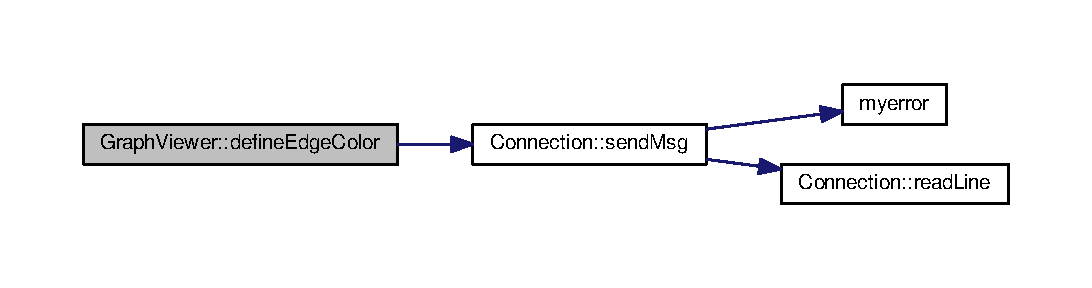
\includegraphics[width=350pt]{classGraphViewer_a4102580b69826ba83251ef7bb262f8be_cgraph}
\end{center}
\end{figure}


\index{Graph\+Viewer@{Graph\+Viewer}!define\+Edge\+Curved@{define\+Edge\+Curved}}
\index{define\+Edge\+Curved@{define\+Edge\+Curved}!Graph\+Viewer@{Graph\+Viewer}}
\subsubsection[{\texorpdfstring{define\+Edge\+Curved(bool curved)}{defineEdgeCurved(bool curved)}}]{\setlength{\rightskip}{0pt plus 5cm}bool Graph\+Viewer\+::define\+Edge\+Curved (
\begin{DoxyParamCaption}
\item[{bool}]{curved}
\end{DoxyParamCaption}
)}\hypertarget{classGraphViewer_a08f362be0e682d91e7506dca8caae1b8}{}\label{classGraphViewer_a08f362be0e682d91e7506dca8caae1b8}
Função que define se as arestas do grafo serão desenhadas como curvas ou retas. Exemplo, para um apontador gv onde foi instanciada a classe \hyperlink{classGraphViewer}{Graph\+Viewer}\+: gv-\/$>$define\+Edge\+Curved(false); faz com que as arestas sejam desenhadas como retas


\begin{DoxyParams}{Parameters}
{\em curved} & Booleano que representa se as arestas serão curvas (true) ou retas (false), sendo o valor por defeito é true. \\
\hline
\end{DoxyParams}


Here is the call graph for this function\+:
\nopagebreak
\begin{figure}[H]
\begin{center}
\leavevmode
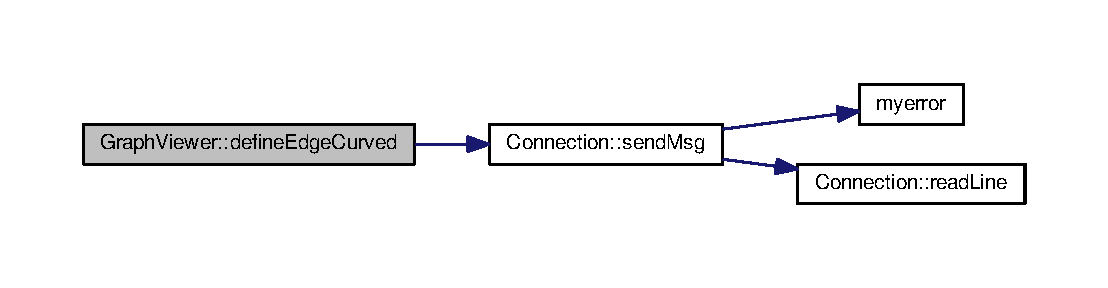
\includegraphics[width=350pt]{classGraphViewer_a08f362be0e682d91e7506dca8caae1b8_cgraph}
\end{center}
\end{figure}


\index{Graph\+Viewer@{Graph\+Viewer}!define\+Edge\+Dashed@{define\+Edge\+Dashed}}
\index{define\+Edge\+Dashed@{define\+Edge\+Dashed}!Graph\+Viewer@{Graph\+Viewer}}
\subsubsection[{\texorpdfstring{define\+Edge\+Dashed(bool dashed)}{defineEdgeDashed(bool dashed)}}]{\setlength{\rightskip}{0pt plus 5cm}bool Graph\+Viewer\+::define\+Edge\+Dashed (
\begin{DoxyParamCaption}
\item[{bool}]{dashed}
\end{DoxyParamCaption}
)}\hypertarget{classGraphViewer_af785279b5c204df0e274b20c36276fc3}{}\label{classGraphViewer_af785279b5c204df0e274b20c36276fc3}
Função que define globalmente se as arestas são desenhadas, ou não, a tracejado. Exemplo, para um apontador gv onde foi instanciada a classe \hyperlink{classGraphViewer}{Graph\+Viewer}\+: gv-\/$>$define\+Edge\+Dashed(true); faz com que por defeito as arestas sejam desenhadas a tracejado


\begin{DoxyParams}{Parameters}
{\em dashed} & Booleano que representa se as arestas vão estar, ou não, todas a tracejado (o valor por defeito é false). \\
\hline
\end{DoxyParams}


Here is the call graph for this function\+:
\nopagebreak
\begin{figure}[H]
\begin{center}
\leavevmode
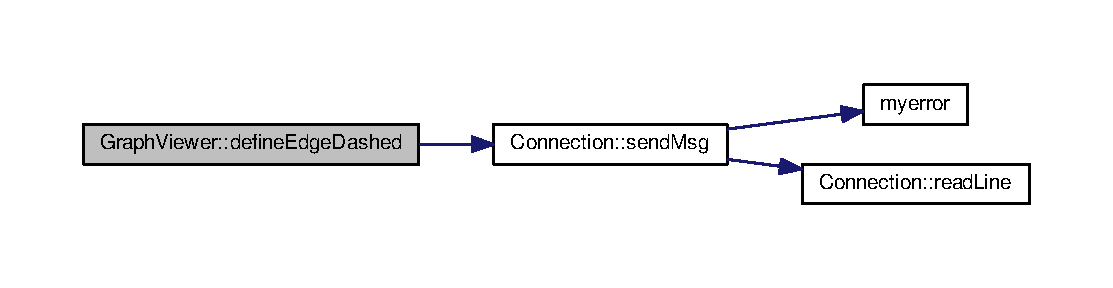
\includegraphics[width=350pt]{classGraphViewer_af785279b5c204df0e274b20c36276fc3_cgraph}
\end{center}
\end{figure}


\index{Graph\+Viewer@{Graph\+Viewer}!define\+Vertex\+Color@{define\+Vertex\+Color}}
\index{define\+Vertex\+Color@{define\+Vertex\+Color}!Graph\+Viewer@{Graph\+Viewer}}
\subsubsection[{\texorpdfstring{define\+Vertex\+Color(string color)}{defineVertexColor(string color)}}]{\setlength{\rightskip}{0pt plus 5cm}bool Graph\+Viewer\+::define\+Vertex\+Color (
\begin{DoxyParamCaption}
\item[{string}]{color}
\end{DoxyParamCaption}
)}\hypertarget{classGraphViewer_a76de8676b7a93d72af514b84cdaa4d21}{}\label{classGraphViewer_a76de8676b7a93d72af514b84cdaa4d21}
Função que define a cor global dos nós. Exemplo, para um apontador gv onde foi instanciada a classe \hyperlink{classGraphViewer}{Graph\+Viewer}\+: gv-\/$>$define\+Vertex\+Color(\+R\+E\+D); modifica a cor por defeito dos nós para vermelho


\begin{DoxyParams}{Parameters}
{\em color} & Nova cor dos nós, utilizar as constantes definidas no \hyperlink{graphviewer_8h}{graphviewer.\+h} para conveniência. \\
\hline
\end{DoxyParams}


Here is the call graph for this function\+:
\nopagebreak
\begin{figure}[H]
\begin{center}
\leavevmode
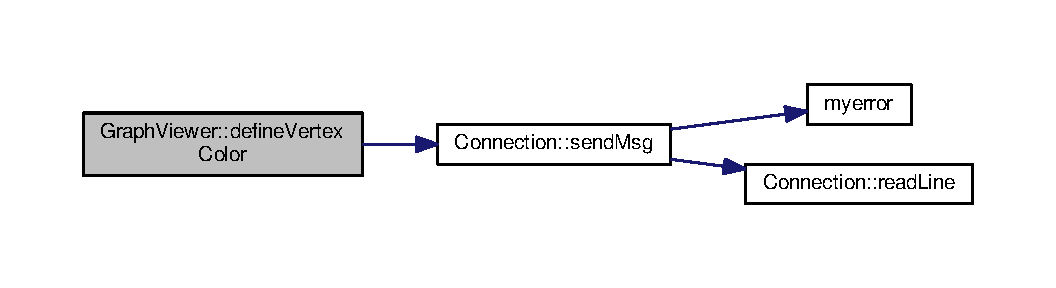
\includegraphics[width=350pt]{classGraphViewer_a76de8676b7a93d72af514b84cdaa4d21_cgraph}
\end{center}
\end{figure}


\index{Graph\+Viewer@{Graph\+Viewer}!define\+Vertex\+Icon@{define\+Vertex\+Icon}}
\index{define\+Vertex\+Icon@{define\+Vertex\+Icon}!Graph\+Viewer@{Graph\+Viewer}}
\subsubsection[{\texorpdfstring{define\+Vertex\+Icon(string filepath)}{defineVertexIcon(string filepath)}}]{\setlength{\rightskip}{0pt plus 5cm}bool Graph\+Viewer\+::define\+Vertex\+Icon (
\begin{DoxyParamCaption}
\item[{string}]{filepath}
\end{DoxyParamCaption}
)}\hypertarget{classGraphViewer_af1adb6a361457187a820e01dcf0a34b7}{}\label{classGraphViewer_af1adb6a361457187a820e01dcf0a34b7}
Função que define um ícone global para os nós. Exemplo, para um apontador gv onde foi instanciada a classe \hyperlink{classGraphViewer}{Graph\+Viewer}\+: gv-\/$>$define\+Vertex\+Icon(\char`\"{}icon.\+gif\char`\"{}); faz com que por defeito os nós, quando desenhados, não sejam um círculo, mas sim a imagem icon.\+gif


\begin{DoxyParams}{Parameters}
{\em filepath} & Caminho do ficheiro a utilizar como novo ícone do nó. \\
\hline
\end{DoxyParams}


Here is the call graph for this function\+:
\nopagebreak
\begin{figure}[H]
\begin{center}
\leavevmode
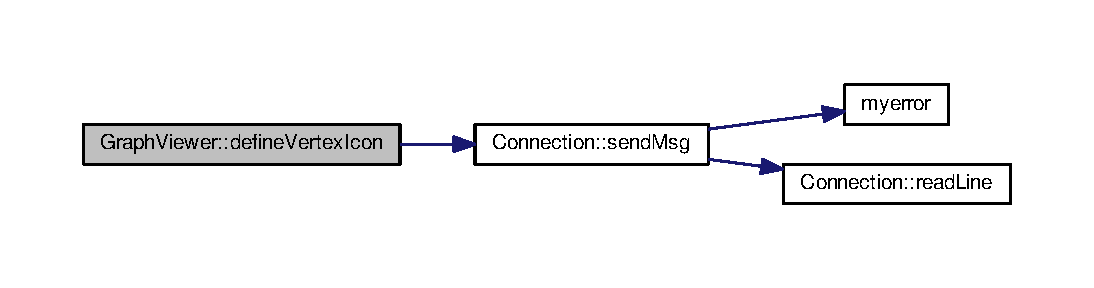
\includegraphics[width=350pt]{classGraphViewer_af1adb6a361457187a820e01dcf0a34b7_cgraph}
\end{center}
\end{figure}


\index{Graph\+Viewer@{Graph\+Viewer}!define\+Vertex\+Size@{define\+Vertex\+Size}}
\index{define\+Vertex\+Size@{define\+Vertex\+Size}!Graph\+Viewer@{Graph\+Viewer}}
\subsubsection[{\texorpdfstring{define\+Vertex\+Size(int size)}{defineVertexSize(int size)}}]{\setlength{\rightskip}{0pt plus 5cm}bool Graph\+Viewer\+::define\+Vertex\+Size (
\begin{DoxyParamCaption}
\item[{int}]{size}
\end{DoxyParamCaption}
)}\hypertarget{classGraphViewer_ac4b2a9fec74d38e64088aa79ca4b7d9b}{}\label{classGraphViewer_ac4b2a9fec74d38e64088aa79ca4b7d9b}
Função que define o tamanho global dos nós. Exemplo, para um apontador gv onde foi instanciada a classe \hyperlink{classGraphViewer}{Graph\+Viewer}\+: gv-\/$>$define\+Vertex\+Size(20); modifica o tamanho por defeito dos nós para 20


\begin{DoxyParams}{Parameters}
{\em size} & Nova cor dos nós, utilizar as constantes definidas no \hyperlink{graphviewer_8h}{graphviewer.\+h} para conveniência. \\
\hline
\end{DoxyParams}


Here is the call graph for this function\+:
\nopagebreak
\begin{figure}[H]
\begin{center}
\leavevmode
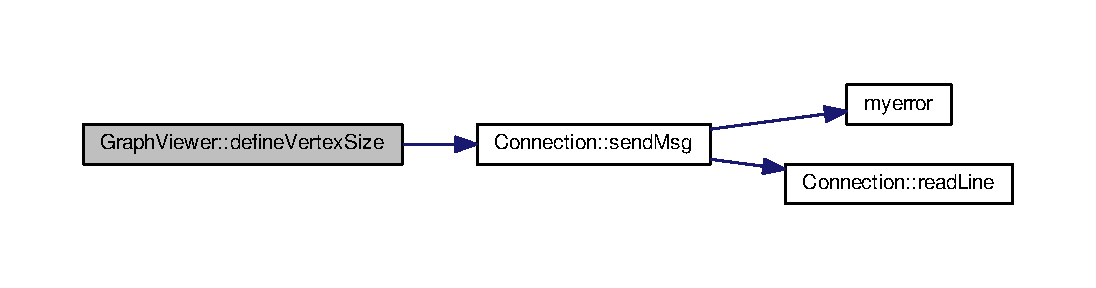
\includegraphics[width=350pt]{classGraphViewer_ac4b2a9fec74d38e64088aa79ca4b7d9b_cgraph}
\end{center}
\end{figure}


\index{Graph\+Viewer@{Graph\+Viewer}!initialize@{initialize}}
\index{initialize@{initialize}!Graph\+Viewer@{Graph\+Viewer}}
\subsubsection[{\texorpdfstring{initialize(int, int, bool, int)}{initialize(int, int, bool, int)}}]{\setlength{\rightskip}{0pt plus 5cm}void Graph\+Viewer\+::initialize (
\begin{DoxyParamCaption}
\item[{int}]{width, }
\item[{int}]{height, }
\item[{bool}]{dynamic, }
\item[{int}]{port\+\_\+n}
\end{DoxyParamCaption}
)\hspace{0.3cm}{\ttfamily [private]}}\hypertarget{classGraphViewer_a1ce9dff4903c650d3b2d33a3ef1d1f61}{}\label{classGraphViewer_a1ce9dff4903c650d3b2d33a3ef1d1f61}


Here is the call graph for this function\+:
\nopagebreak
\begin{figure}[H]
\begin{center}
\leavevmode
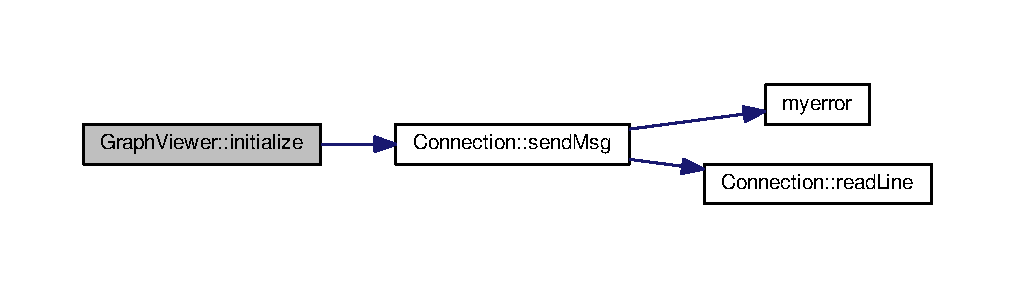
\includegraphics[width=350pt]{classGraphViewer_a1ce9dff4903c650d3b2d33a3ef1d1f61_cgraph}
\end{center}
\end{figure}


\index{Graph\+Viewer@{Graph\+Viewer}!rearrange@{rearrange}}
\index{rearrange@{rearrange}!Graph\+Viewer@{Graph\+Viewer}}
\subsubsection[{\texorpdfstring{rearrange()}{rearrange()}}]{\setlength{\rightskip}{0pt plus 5cm}bool Graph\+Viewer\+::rearrange (
\begin{DoxyParamCaption}
{}
\end{DoxyParamCaption}
)}\hypertarget{classGraphViewer_a3009a66958686ccb7e78b68e37c3c423}{}\label{classGraphViewer_a3009a66958686ccb7e78b68e37c3c423}
Função que actualiza a visualização do grafo. 

Here is the call graph for this function\+:
\nopagebreak
\begin{figure}[H]
\begin{center}
\leavevmode
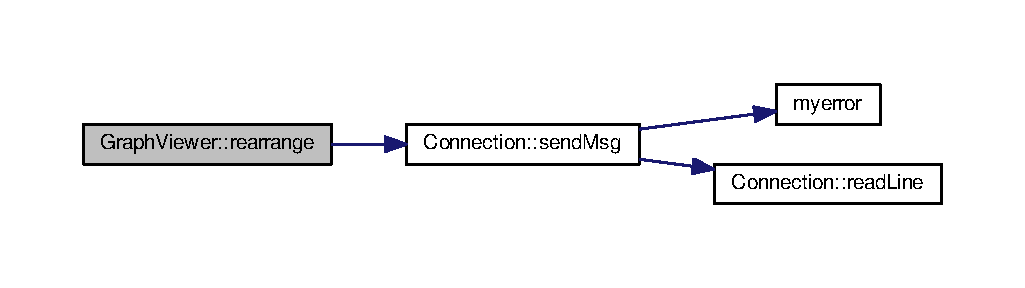
\includegraphics[width=350pt]{classGraphViewer_a3009a66958686ccb7e78b68e37c3c423_cgraph}
\end{center}
\end{figure}


\index{Graph\+Viewer@{Graph\+Viewer}!remove\+Edge@{remove\+Edge}}
\index{remove\+Edge@{remove\+Edge}!Graph\+Viewer@{Graph\+Viewer}}
\subsubsection[{\texorpdfstring{remove\+Edge(int id)}{removeEdge(int id)}}]{\setlength{\rightskip}{0pt plus 5cm}bool Graph\+Viewer\+::remove\+Edge (
\begin{DoxyParamCaption}
\item[{int}]{id}
\end{DoxyParamCaption}
)}\hypertarget{classGraphViewer_a9a8ee68c7c12b373affbe4069dd95d72}{}\label{classGraphViewer_a9a8ee68c7c12b373affbe4069dd95d72}
Remove uma aresta da representação do grafo. Exemplo, para um apontador gv onde foi instanciada a classe \hyperlink{classGraphViewer}{Graph\+Viewer}\+: gv-\/$>$remove\+Edge(0) remove a aresta com ID 0


\begin{DoxyParams}{Parameters}
{\em id} & Identificador único da aresta a remover. \\
\hline
\end{DoxyParams}


Here is the call graph for this function\+:
\nopagebreak
\begin{figure}[H]
\begin{center}
\leavevmode
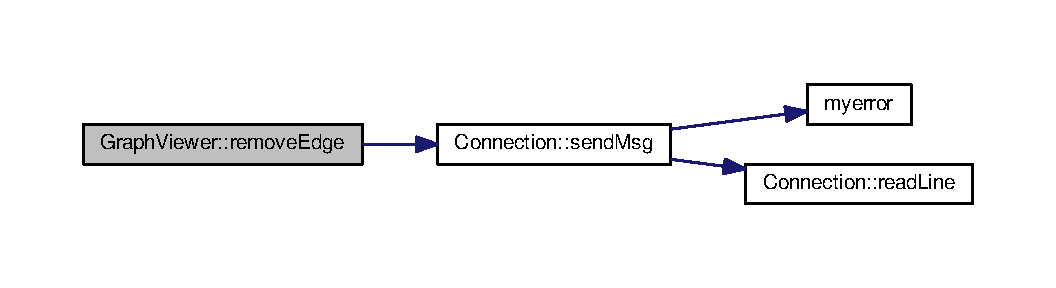
\includegraphics[width=350pt]{classGraphViewer_a9a8ee68c7c12b373affbe4069dd95d72_cgraph}
\end{center}
\end{figure}


\index{Graph\+Viewer@{Graph\+Viewer}!remove\+Node@{remove\+Node}}
\index{remove\+Node@{remove\+Node}!Graph\+Viewer@{Graph\+Viewer}}
\subsubsection[{\texorpdfstring{remove\+Node(int id)}{removeNode(int id)}}]{\setlength{\rightskip}{0pt plus 5cm}bool Graph\+Viewer\+::remove\+Node (
\begin{DoxyParamCaption}
\item[{int}]{id}
\end{DoxyParamCaption}
)}\hypertarget{classGraphViewer_a0c418639bb911eb827cabf895915f775}{}\label{classGraphViewer_a0c418639bb911eb827cabf895915f775}
Remove um nó da representação do grafo e todas as arestas ligadas a este. Exemplo, para um apontador gv onde foi instanciada a classe \hyperlink{classGraphViewer}{Graph\+Viewer}\+: gv-\/$>$remove\+Node(0) remove o nó com ID 0


\begin{DoxyParams}{Parameters}
{\em id} & Identificador único do nó a a remover. \\
\hline
\end{DoxyParams}


Here is the call graph for this function\+:
\nopagebreak
\begin{figure}[H]
\begin{center}
\leavevmode
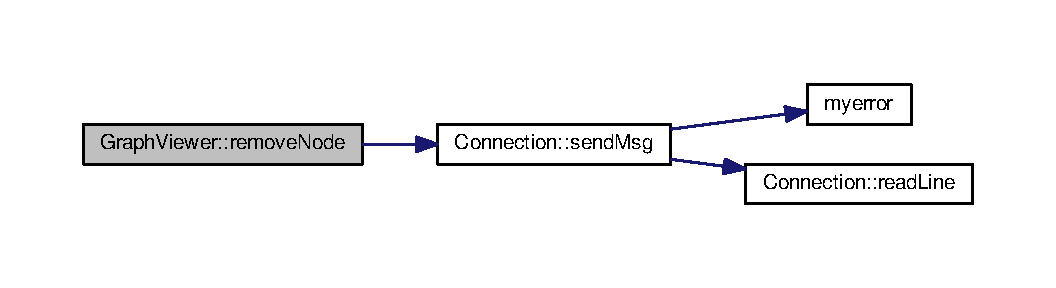
\includegraphics[width=350pt]{classGraphViewer_a0c418639bb911eb827cabf895915f775_cgraph}
\end{center}
\end{figure}


\index{Graph\+Viewer@{Graph\+Viewer}!reset\+Edge\+Color@{reset\+Edge\+Color}}
\index{reset\+Edge\+Color@{reset\+Edge\+Color}!Graph\+Viewer@{Graph\+Viewer}}
\subsubsection[{\texorpdfstring{reset\+Edge\+Color()}{resetEdgeColor()}}]{\setlength{\rightskip}{0pt plus 5cm}bool Graph\+Viewer\+::reset\+Edge\+Color (
\begin{DoxyParamCaption}
{}
\end{DoxyParamCaption}
)}\hypertarget{classGraphViewer_a1df1a30f4668bf70364fac232f8d0600}{}\label{classGraphViewer_a1df1a30f4668bf70364fac232f8d0600}
Função que restaura a cor global das arestas. 

Here is the call graph for this function\+:
\nopagebreak
\begin{figure}[H]
\begin{center}
\leavevmode
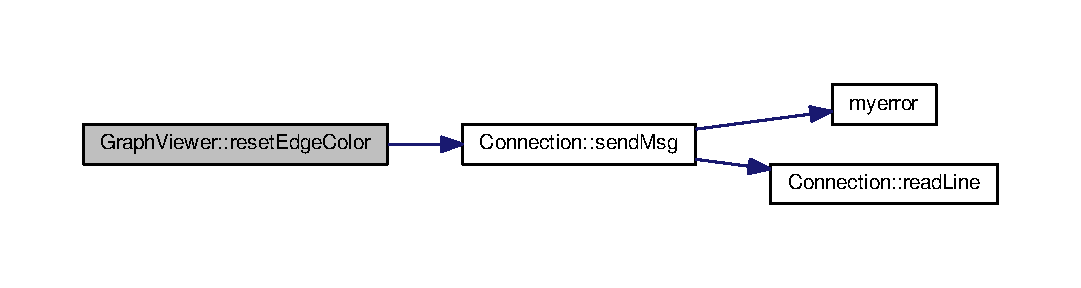
\includegraphics[width=350pt]{classGraphViewer_a1df1a30f4668bf70364fac232f8d0600_cgraph}
\end{center}
\end{figure}


\index{Graph\+Viewer@{Graph\+Viewer}!reset\+Vertex\+Color@{reset\+Vertex\+Color}}
\index{reset\+Vertex\+Color@{reset\+Vertex\+Color}!Graph\+Viewer@{Graph\+Viewer}}
\subsubsection[{\texorpdfstring{reset\+Vertex\+Color()}{resetVertexColor()}}]{\setlength{\rightskip}{0pt plus 5cm}bool Graph\+Viewer\+::reset\+Vertex\+Color (
\begin{DoxyParamCaption}
{}
\end{DoxyParamCaption}
)}\hypertarget{classGraphViewer_acd95eee309d5e9b1935ec39c5ed45cac}{}\label{classGraphViewer_acd95eee309d5e9b1935ec39c5ed45cac}
Função que restaura a cor global dos nós. 

Here is the call graph for this function\+:
\nopagebreak
\begin{figure}[H]
\begin{center}
\leavevmode
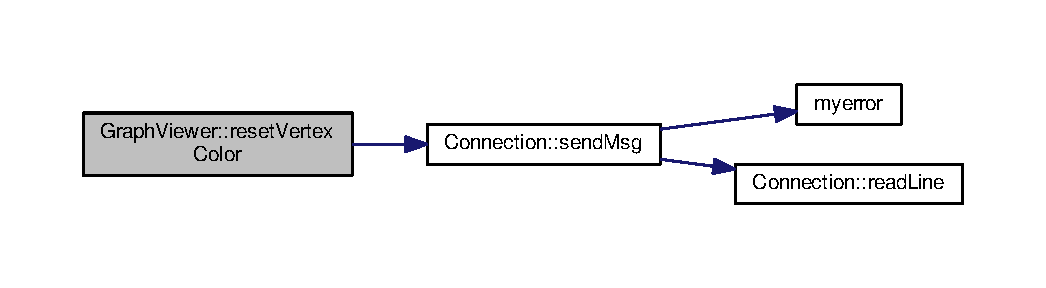
\includegraphics[width=350pt]{classGraphViewer_acd95eee309d5e9b1935ec39c5ed45cac_cgraph}
\end{center}
\end{figure}


\index{Graph\+Viewer@{Graph\+Viewer}!reset\+Vertex\+Icon@{reset\+Vertex\+Icon}}
\index{reset\+Vertex\+Icon@{reset\+Vertex\+Icon}!Graph\+Viewer@{Graph\+Viewer}}
\subsubsection[{\texorpdfstring{reset\+Vertex\+Icon()}{resetVertexIcon()}}]{\setlength{\rightskip}{0pt plus 5cm}bool Graph\+Viewer\+::reset\+Vertex\+Icon (
\begin{DoxyParamCaption}
{}
\end{DoxyParamCaption}
)}\hypertarget{classGraphViewer_ae2b602cfdfb49ec0a67f2bcd11b0fbdb}{}\label{classGraphViewer_ae2b602cfdfb49ec0a67f2bcd11b0fbdb}
Função que apaga o ícone global para os nós. 

Here is the call graph for this function\+:
\nopagebreak
\begin{figure}[H]
\begin{center}
\leavevmode
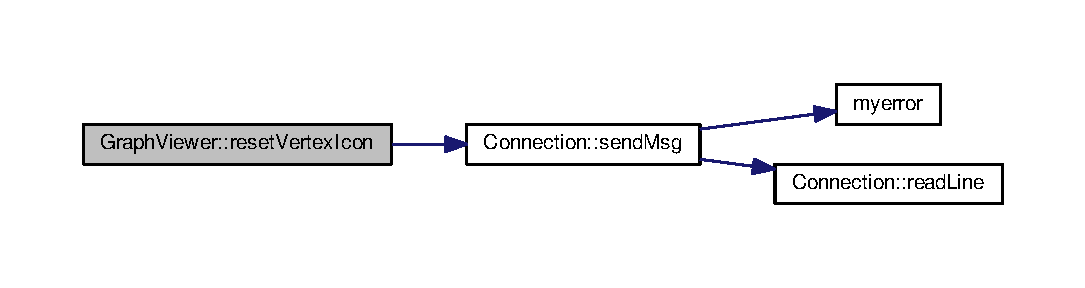
\includegraphics[width=350pt]{classGraphViewer_ae2b602cfdfb49ec0a67f2bcd11b0fbdb_cgraph}
\end{center}
\end{figure}


\index{Graph\+Viewer@{Graph\+Viewer}!set\+Background@{set\+Background}}
\index{set\+Background@{set\+Background}!Graph\+Viewer@{Graph\+Viewer}}
\subsubsection[{\texorpdfstring{set\+Background(string path)}{setBackground(string path)}}]{\setlength{\rightskip}{0pt plus 5cm}bool Graph\+Viewer\+::set\+Background (
\begin{DoxyParamCaption}
\item[{string}]{path}
\end{DoxyParamCaption}
)}\hypertarget{classGraphViewer_a02437b5fecd8b90de24436068312d593}{}\label{classGraphViewer_a02437b5fecd8b90de24436068312d593}
Função que altera a imagem de fundo do grafo. Exemplo, para um apontador gv onde foi instanciada a classe \hyperlink{classGraphViewer}{Graph\+Viewer}\+: gv-\/$>$set\+Back\+Ground(\char`\"{}fundo.\+png\char`\"{}); faz com que o fundo da janela seja a imagem fundo.\+png, em vez de cinzento


\begin{DoxyParams}{Parameters}
{\em path} & Caminho para o ficheiro com a imagem. \\
\hline
\end{DoxyParams}


Here is the call graph for this function\+:
\nopagebreak
\begin{figure}[H]
\begin{center}
\leavevmode
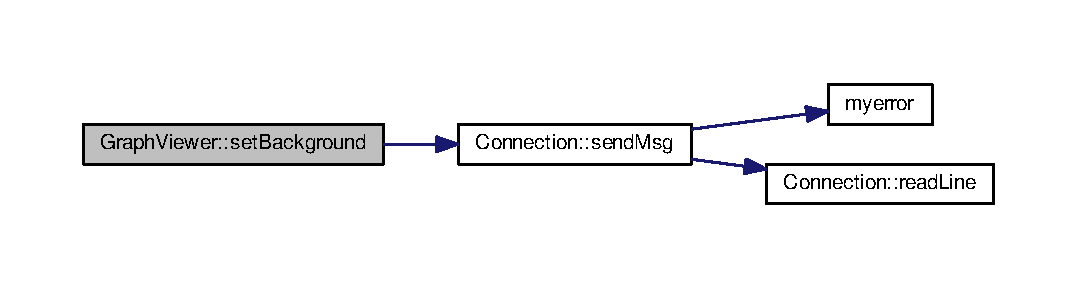
\includegraphics[width=350pt]{classGraphViewer_a02437b5fecd8b90de24436068312d593_cgraph}
\end{center}
\end{figure}


\index{Graph\+Viewer@{Graph\+Viewer}!set\+Edge\+Color@{set\+Edge\+Color}}
\index{set\+Edge\+Color@{set\+Edge\+Color}!Graph\+Viewer@{Graph\+Viewer}}
\subsubsection[{\texorpdfstring{set\+Edge\+Color(int id, string color)}{setEdgeColor(int id, string color)}}]{\setlength{\rightskip}{0pt plus 5cm}bool Graph\+Viewer\+::set\+Edge\+Color (
\begin{DoxyParamCaption}
\item[{int}]{id, }
\item[{string}]{color}
\end{DoxyParamCaption}
)}\hypertarget{classGraphViewer_a07ccc96707efae4aa5f3ced3dca015af}{}\label{classGraphViewer_a07ccc96707efae4aa5f3ced3dca015af}
Função que define a cor de uma aresta. Exemplo, para um apontador gv onde foi instanciada a classe \hyperlink{classGraphViewer}{Graph\+Viewer}\+: gv-\/$>$set\+Edge\+Color(0, B\+L\+U\+E); modifica a cor da aresta com ID 0 para azul


\begin{DoxyParams}{Parameters}
{\em id} & Identificador único da aresta com a cor a alterar. \\
\hline
{\em color} & Nova cor da aresta, utilizar as constantes definidas no \hyperlink{graphviewer_8h}{graphviewer.\+h} para conveniência. \\
\hline
\end{DoxyParams}


Here is the call graph for this function\+:
\nopagebreak
\begin{figure}[H]
\begin{center}
\leavevmode
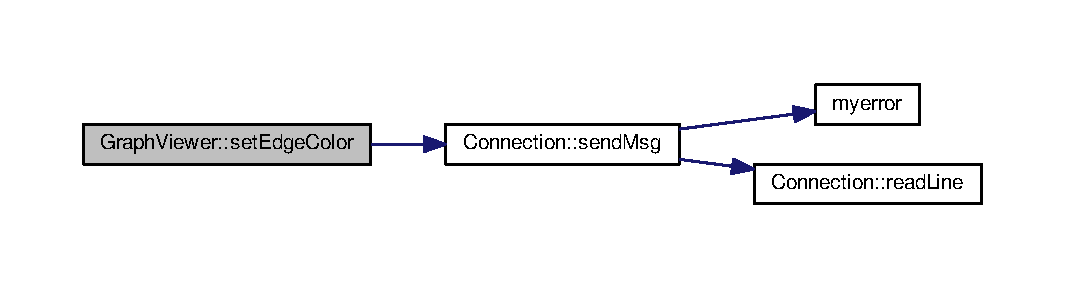
\includegraphics[width=350pt]{classGraphViewer_a07ccc96707efae4aa5f3ced3dca015af_cgraph}
\end{center}
\end{figure}


\index{Graph\+Viewer@{Graph\+Viewer}!set\+Edge\+Dashed@{set\+Edge\+Dashed}}
\index{set\+Edge\+Dashed@{set\+Edge\+Dashed}!Graph\+Viewer@{Graph\+Viewer}}
\subsubsection[{\texorpdfstring{set\+Edge\+Dashed(int id, bool dashed)}{setEdgeDashed(int id, bool dashed)}}]{\setlength{\rightskip}{0pt plus 5cm}bool Graph\+Viewer\+::set\+Edge\+Dashed (
\begin{DoxyParamCaption}
\item[{int}]{id, }
\item[{bool}]{dashed}
\end{DoxyParamCaption}
)}\hypertarget{classGraphViewer_a1698f1c6b3a8e7cabc7b7d7cf42fc7f0}{}\label{classGraphViewer_a1698f1c6b3a8e7cabc7b7d7cf42fc7f0}
Função que define se uma aresta é desenhada, ou não, a tracejado. Exemplo, para um apontador gv onde foi instanciada a classe \hyperlink{classGraphViewer}{Graph\+Viewer}\+: gv-\/$>$set\+Edge\+Dashed(0, false); faz com que a aresta com ID 0 seja desenhada a traço contínuo


\begin{DoxyParams}{Parameters}
{\em id} & Identificador único da aresta com a cor a alterar. \\
\hline
{\em dashed} & Nova cor da aresta, utilizar as constantes definidas no \hyperlink{graphviewer_8h}{graphviewer.\+h} para conveniência. \\
\hline
\end{DoxyParams}


Here is the call graph for this function\+:
\nopagebreak
\begin{figure}[H]
\begin{center}
\leavevmode
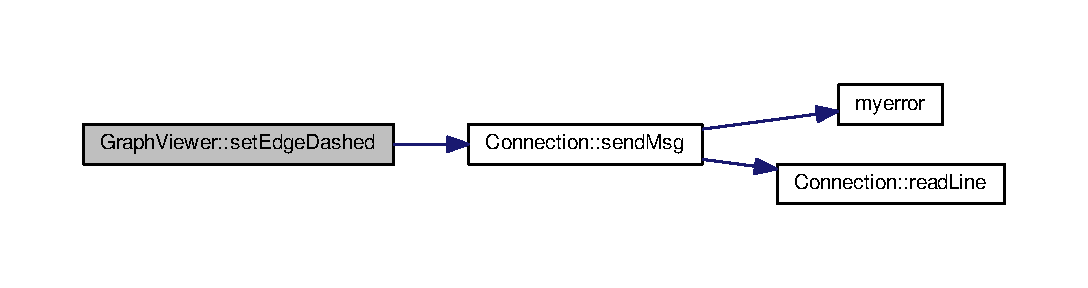
\includegraphics[width=350pt]{classGraphViewer_a1698f1c6b3a8e7cabc7b7d7cf42fc7f0_cgraph}
\end{center}
\end{figure}


\index{Graph\+Viewer@{Graph\+Viewer}!set\+Edge\+Flow@{set\+Edge\+Flow}}
\index{set\+Edge\+Flow@{set\+Edge\+Flow}!Graph\+Viewer@{Graph\+Viewer}}
\subsubsection[{\texorpdfstring{set\+Edge\+Flow(int id, int flow)}{setEdgeFlow(int id, int flow)}}]{\setlength{\rightskip}{0pt plus 5cm}bool Graph\+Viewer\+::set\+Edge\+Flow (
\begin{DoxyParamCaption}
\item[{int}]{id, }
\item[{int}]{flow}
\end{DoxyParamCaption}
)}\hypertarget{classGraphViewer_a69eb065145063e4dea41961e92e35c8e}{}\label{classGraphViewer_a69eb065145063e4dea41961e92e35c8e}
Função que define o fluxo de uma aresta na representação do grafo, a ser visualizado como f\+: valor\+\_\+do\+\_\+fluxo, precedido pelo peso e seguido por texto definido pelo utilizador. Exemplo, para um apontador gv onde foi instanciada a classe \hyperlink{classGraphViewer}{Graph\+Viewer}\+: gv-\/$>$set\+Edge\+Flow(0, 20); modifica o fluxo da aresta com ID 0 para 20


\begin{DoxyParams}{Parameters}
{\em id} & Identificador único da aresta a modificar. \\
\hline
{\em flow} & Fluxo associado à aresta. \\
\hline
\end{DoxyParams}


Here is the call graph for this function\+:
\nopagebreak
\begin{figure}[H]
\begin{center}
\leavevmode
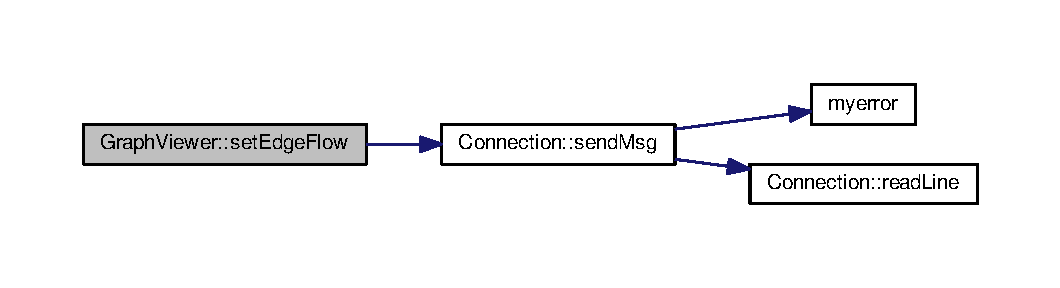
\includegraphics[width=350pt]{classGraphViewer_a69eb065145063e4dea41961e92e35c8e_cgraph}
\end{center}
\end{figure}


\index{Graph\+Viewer@{Graph\+Viewer}!set\+Edge\+Label@{set\+Edge\+Label}}
\index{set\+Edge\+Label@{set\+Edge\+Label}!Graph\+Viewer@{Graph\+Viewer}}
\subsubsection[{\texorpdfstring{set\+Edge\+Label(int id, string label)}{setEdgeLabel(int id, string label)}}]{\setlength{\rightskip}{0pt plus 5cm}bool Graph\+Viewer\+::set\+Edge\+Label (
\begin{DoxyParamCaption}
\item[{int}]{id, }
\item[{string}]{label}
\end{DoxyParamCaption}
)}\hypertarget{classGraphViewer_a447cca0064e785654c2105602c2961ca}{}\label{classGraphViewer_a447cca0064e785654c2105602c2961ca}
Função que define o texto de uma aresta. Exemplo, para um apontador gv onde foi instanciada a classe \hyperlink{classGraphViewer}{Graph\+Viewer}\+: gv-\/$>$set\+Edge\+Label(0, \char`\"{}\+Isto é uma aresta\char`\"{}); adiciona o texto \char`\"{}\+Isto é uma aresta\char`\"{} à aresta com ID 0


\begin{DoxyParams}{Parameters}
{\em id} & Identificador único da aresta com o texto a alterar. \\
\hline
{\em label} & Novo texto da aresta. \\
\hline
\end{DoxyParams}


Here is the call graph for this function\+:
\nopagebreak
\begin{figure}[H]
\begin{center}
\leavevmode
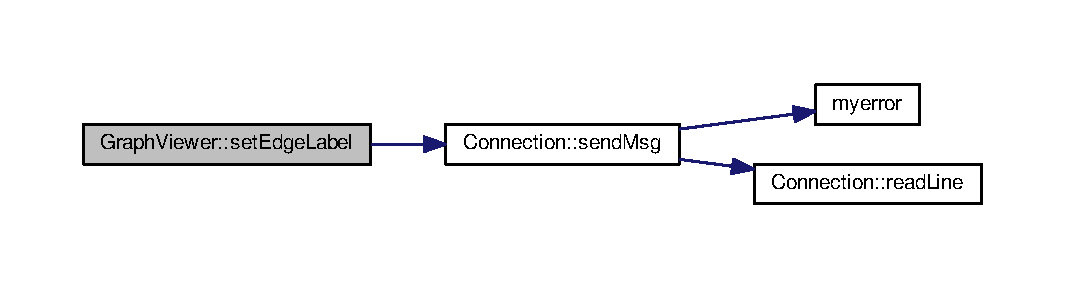
\includegraphics[width=350pt]{classGraphViewer_a447cca0064e785654c2105602c2961ca_cgraph}
\end{center}
\end{figure}


\index{Graph\+Viewer@{Graph\+Viewer}!set\+Edge\+Thickness@{set\+Edge\+Thickness}}
\index{set\+Edge\+Thickness@{set\+Edge\+Thickness}!Graph\+Viewer@{Graph\+Viewer}}
\subsubsection[{\texorpdfstring{set\+Edge\+Thickness(int id, int thickness)}{setEdgeThickness(int id, int thickness)}}]{\setlength{\rightskip}{0pt plus 5cm}bool Graph\+Viewer\+::set\+Edge\+Thickness (
\begin{DoxyParamCaption}
\item[{int}]{id, }
\item[{int}]{thickness}
\end{DoxyParamCaption}
)}\hypertarget{classGraphViewer_a07f598272fe3515455eab13be749604a}{}\label{classGraphViewer_a07f598272fe3515455eab13be749604a}
Função que define a espessura de uma aresta. Exemplo, para um apontador gv onde foi instanciada a classe \hyperlink{classGraphViewer}{Graph\+Viewer}\+: gv-\/$>$set\+Edge\+Thickness(0, 20); modifica a espessura da aresta com ID 0 para 20


\begin{DoxyParams}{Parameters}
{\em id} & Identificador único da aresta com a espessura a alterar. \\
\hline
{\em thickness} & Nova espessura da aresta, sendo que por base, as arestas são criadas com a espessura de 1. \\
\hline
\end{DoxyParams}


Here is the call graph for this function\+:
\nopagebreak
\begin{figure}[H]
\begin{center}
\leavevmode
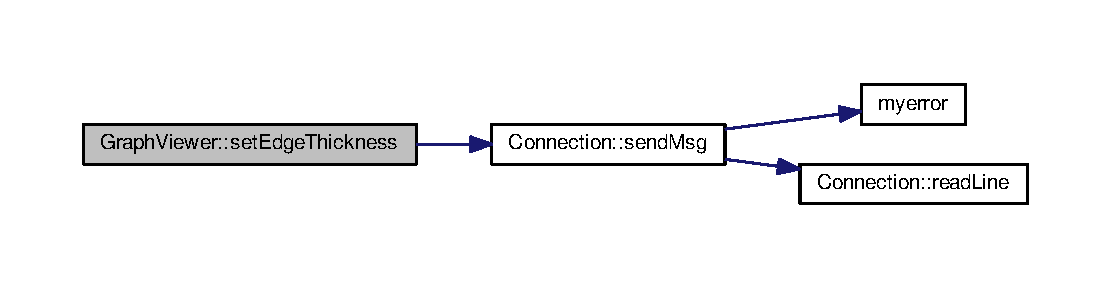
\includegraphics[width=350pt]{classGraphViewer_a07f598272fe3515455eab13be749604a_cgraph}
\end{center}
\end{figure}


\index{Graph\+Viewer@{Graph\+Viewer}!set\+Edge\+Weight@{set\+Edge\+Weight}}
\index{set\+Edge\+Weight@{set\+Edge\+Weight}!Graph\+Viewer@{Graph\+Viewer}}
\subsubsection[{\texorpdfstring{set\+Edge\+Weight(int id, int weight)}{setEdgeWeight(int id, int weight)}}]{\setlength{\rightskip}{0pt plus 5cm}bool Graph\+Viewer\+::set\+Edge\+Weight (
\begin{DoxyParamCaption}
\item[{int}]{id, }
\item[{int}]{weight}
\end{DoxyParamCaption}
)}\hypertarget{classGraphViewer_ac211de009a0afe2e6d44f4f8d030a2cc}{}\label{classGraphViewer_ac211de009a0afe2e6d44f4f8d030a2cc}
Função que define o peso de uma aresta na representação do grafo, a ser visualizado como w\+: valor\+\_\+do\+\_\+peso, seguido de qualquer outro texto associado à aresta. Exemplo, para um apontador gv onde foi instanciada a classe \hyperlink{classGraphViewer}{Graph\+Viewer}\+: gv-\/$>$set\+Edge\+Weight(0, 20); modifica o peso da aresta com ID 0 para 20


\begin{DoxyParams}{Parameters}
{\em id} & Identificador único da aresta a modificar. \\
\hline
{\em weight} & Peso associado à aresta. \\
\hline
\end{DoxyParams}


Here is the call graph for this function\+:
\nopagebreak
\begin{figure}[H]
\begin{center}
\leavevmode
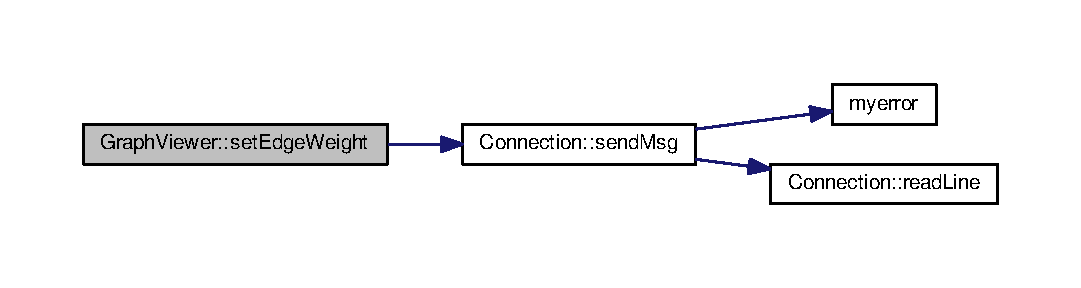
\includegraphics[width=350pt]{classGraphViewer_ac211de009a0afe2e6d44f4f8d030a2cc_cgraph}
\end{center}
\end{figure}


\index{Graph\+Viewer@{Graph\+Viewer}!set\+Vertex\+Color@{set\+Vertex\+Color}}
\index{set\+Vertex\+Color@{set\+Vertex\+Color}!Graph\+Viewer@{Graph\+Viewer}}
\subsubsection[{\texorpdfstring{set\+Vertex\+Color(int id, string color)}{setVertexColor(int id, string color)}}]{\setlength{\rightskip}{0pt plus 5cm}bool Graph\+Viewer\+::set\+Vertex\+Color (
\begin{DoxyParamCaption}
\item[{int}]{id, }
\item[{string}]{color}
\end{DoxyParamCaption}
)}\hypertarget{classGraphViewer_a8b542d7e09e81a45a74760c19233beb0}{}\label{classGraphViewer_a8b542d7e09e81a45a74760c19233beb0}
Função que define a cor de um nó. Exemplo, para um apontador gv onde foi instanciada a classe \hyperlink{classGraphViewer}{Graph\+Viewer}\+: gv-\/$>$set\+Vertex\+Color(0, G\+R\+E\+E\+N); modifica a cor do nó com ID 0 para verde


\begin{DoxyParams}{Parameters}
{\em id} & Identificador único do nó com a cor a alterar. \\
\hline
{\em color} & Nova cor do nó, utilizar as constantes definidas no \hyperlink{graphviewer_8h}{graphviewer.\+h} para conveniência. \\
\hline
\end{DoxyParams}


Here is the call graph for this function\+:
\nopagebreak
\begin{figure}[H]
\begin{center}
\leavevmode
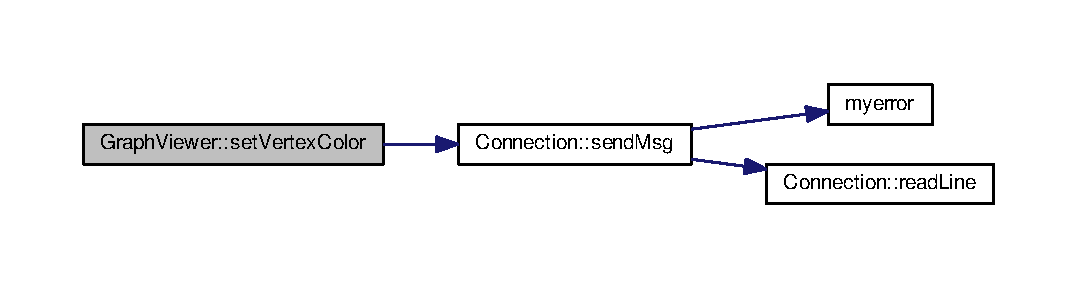
\includegraphics[width=350pt]{classGraphViewer_a8b542d7e09e81a45a74760c19233beb0_cgraph}
\end{center}
\end{figure}


\index{Graph\+Viewer@{Graph\+Viewer}!set\+Vertex\+Icon@{set\+Vertex\+Icon}}
\index{set\+Vertex\+Icon@{set\+Vertex\+Icon}!Graph\+Viewer@{Graph\+Viewer}}
\subsubsection[{\texorpdfstring{set\+Vertex\+Icon(int id, string filepath)}{setVertexIcon(int id, string filepath)}}]{\setlength{\rightskip}{0pt plus 5cm}bool Graph\+Viewer\+::set\+Vertex\+Icon (
\begin{DoxyParamCaption}
\item[{int}]{id, }
\item[{string}]{filepath}
\end{DoxyParamCaption}
)}\hypertarget{classGraphViewer_a02d5f7393eab9a2d1b66719039597a64}{}\label{classGraphViewer_a02d5f7393eab9a2d1b66719039597a64}
Função que define um ícone para um nó. Exemplo, para um apontador gv onde foi instanciada a classe \hyperlink{classGraphViewer}{Graph\+Viewer}\+: gv-\/$>$set\+Vertex\+Icon(0, \char`\"{}icon.\+png\char`\"{}); faz com que o nó, quando desenhado, não seja um círculo, mas sim a imagem icon.\+png


\begin{DoxyParams}{Parameters}
{\em id} & Identificador único do nó com o ícone a alterar. \\
\hline
{\em filepath} & Caminho do ficheiro a utilizar como novo ícone do nó. \\
\hline
\end{DoxyParams}


Here is the call graph for this function\+:
\nopagebreak
\begin{figure}[H]
\begin{center}
\leavevmode
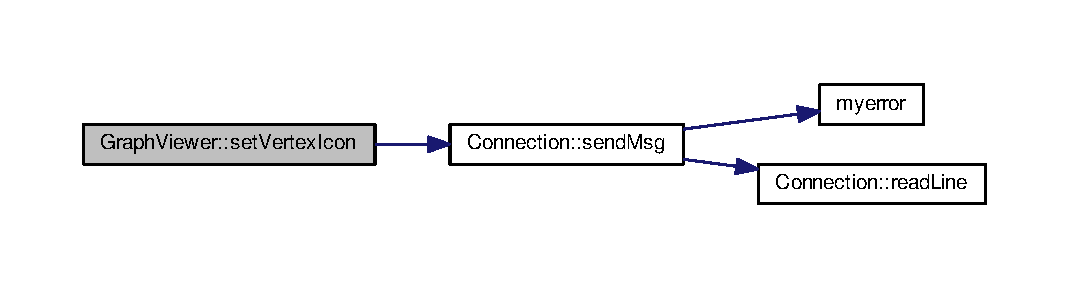
\includegraphics[width=350pt]{classGraphViewer_a02d5f7393eab9a2d1b66719039597a64_cgraph}
\end{center}
\end{figure}


\index{Graph\+Viewer@{Graph\+Viewer}!set\+Vertex\+Label@{set\+Vertex\+Label}}
\index{set\+Vertex\+Label@{set\+Vertex\+Label}!Graph\+Viewer@{Graph\+Viewer}}
\subsubsection[{\texorpdfstring{set\+Vertex\+Label(int id, string label)}{setVertexLabel(int id, string label)}}]{\setlength{\rightskip}{0pt plus 5cm}bool Graph\+Viewer\+::set\+Vertex\+Label (
\begin{DoxyParamCaption}
\item[{int}]{id, }
\item[{string}]{label}
\end{DoxyParamCaption}
)}\hypertarget{classGraphViewer_ac25d7d007022fda16799808ba136e909}{}\label{classGraphViewer_ac25d7d007022fda16799808ba136e909}
Função que define o texto de um nó. Exemplo, para um apontador gv onde foi instanciada a classe \hyperlink{classGraphViewer}{Graph\+Viewer}\+: gv-\/$>$set\+Vertex\+Label(0, \char`\"{}\+Isto é um nó\char`\"{}); adiciona o texto \char`\"{}\+Isto é um nó\char`\"{} ao nó com ID 0


\begin{DoxyParams}{Parameters}
{\em id} & Identificador único do nó com o texto a alterar. \\
\hline
{\em label} & Novo texto do nó. \\
\hline
\end{DoxyParams}


Here is the call graph for this function\+:
\nopagebreak
\begin{figure}[H]
\begin{center}
\leavevmode
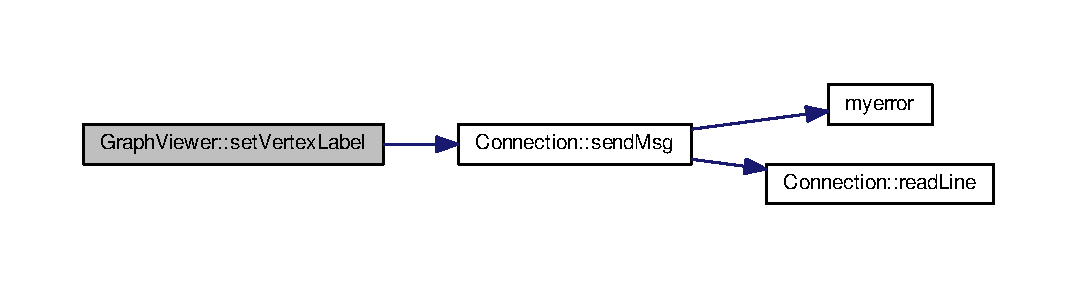
\includegraphics[width=350pt]{classGraphViewer_ac25d7d007022fda16799808ba136e909_cgraph}
\end{center}
\end{figure}


\index{Graph\+Viewer@{Graph\+Viewer}!set\+Vertex\+Size@{set\+Vertex\+Size}}
\index{set\+Vertex\+Size@{set\+Vertex\+Size}!Graph\+Viewer@{Graph\+Viewer}}
\subsubsection[{\texorpdfstring{set\+Vertex\+Size(int id, int size)}{setVertexSize(int id, int size)}}]{\setlength{\rightskip}{0pt plus 5cm}bool Graph\+Viewer\+::set\+Vertex\+Size (
\begin{DoxyParamCaption}
\item[{int}]{id, }
\item[{int}]{size}
\end{DoxyParamCaption}
)}\hypertarget{classGraphViewer_ae930dfdfcdeb7a871eefb6028d74b9f9}{}\label{classGraphViewer_ae930dfdfcdeb7a871eefb6028d74b9f9}
Função que define o tamanho de um nó. Exemplo, para um apontador gv onde foi instanciada a classe \hyperlink{classGraphViewer}{Graph\+Viewer}\+: gv-\/$>$set\+Vertex\+Size(0, 10); modifica o tamanho do nó com ID 0 para 40


\begin{DoxyParams}{Parameters}
{\em id} & Identificador único do nó com o tamanho a alterar. \\
\hline
{\em size} & Novo tamanho do nó. \\
\hline
\end{DoxyParams}


Here is the call graph for this function\+:
\nopagebreak
\begin{figure}[H]
\begin{center}
\leavevmode
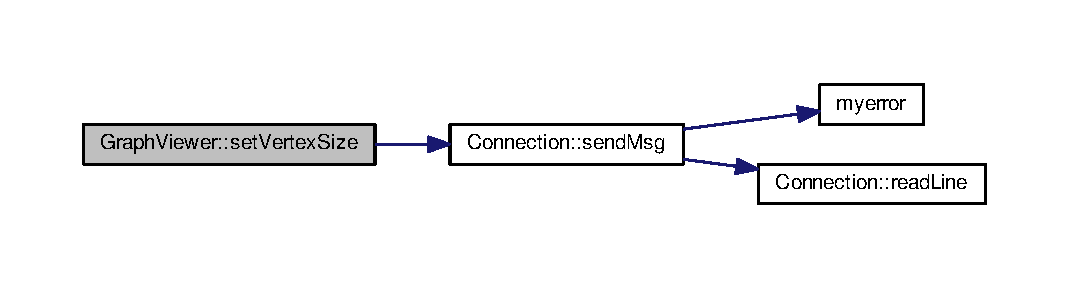
\includegraphics[width=350pt]{classGraphViewer_ae930dfdfcdeb7a871eefb6028d74b9f9_cgraph}
\end{center}
\end{figure}




\subsection{Member Data Documentation}
\index{Graph\+Viewer@{Graph\+Viewer}!con@{con}}
\index{con@{con}!Graph\+Viewer@{Graph\+Viewer}}
\subsubsection[{\texorpdfstring{con}{con}}]{\setlength{\rightskip}{0pt plus 5cm}{\bf Connection}$\ast$ Graph\+Viewer\+::con\hspace{0.3cm}{\ttfamily [private]}}\hypertarget{classGraphViewer_a14a206f78c242e739e0908b06070ba4d}{}\label{classGraphViewer_a14a206f78c242e739e0908b06070ba4d}
\index{Graph\+Viewer@{Graph\+Viewer}!height@{height}}
\index{height@{height}!Graph\+Viewer@{Graph\+Viewer}}
\subsubsection[{\texorpdfstring{height}{height}}]{\setlength{\rightskip}{0pt plus 5cm}int Graph\+Viewer\+::height\hspace{0.3cm}{\ttfamily [private]}}\hypertarget{classGraphViewer_a9a1000e492a66ac4301c7135275690da}{}\label{classGraphViewer_a9a1000e492a66ac4301c7135275690da}
\index{Graph\+Viewer@{Graph\+Viewer}!is\+Dynamic@{is\+Dynamic}}
\index{is\+Dynamic@{is\+Dynamic}!Graph\+Viewer@{Graph\+Viewer}}
\subsubsection[{\texorpdfstring{is\+Dynamic}{isDynamic}}]{\setlength{\rightskip}{0pt plus 5cm}bool Graph\+Viewer\+::is\+Dynamic\hspace{0.3cm}{\ttfamily [private]}}\hypertarget{classGraphViewer_a9d9947154bc63354c6d02a0680aad952}{}\label{classGraphViewer_a9d9947154bc63354c6d02a0680aad952}
\index{Graph\+Viewer@{Graph\+Viewer}!port@{port}}
\index{port@{port}!Graph\+Viewer@{Graph\+Viewer}}
\subsubsection[{\texorpdfstring{port}{port}}]{\setlength{\rightskip}{0pt plus 5cm}short Graph\+Viewer\+::port = 7772\hspace{0.3cm}{\ttfamily [static]}}\hypertarget{classGraphViewer_a89d0abe75f41feededc49497cc514342}{}\label{classGraphViewer_a89d0abe75f41feededc49497cc514342}
Variável que guarda a próxima porta que o programa vai usar. O valor inicial é 7772. \index{Graph\+Viewer@{Graph\+Viewer}!width@{width}}
\index{width@{width}!Graph\+Viewer@{Graph\+Viewer}}
\subsubsection[{\texorpdfstring{width}{width}}]{\setlength{\rightskip}{0pt plus 5cm}int Graph\+Viewer\+::width\hspace{0.3cm}{\ttfamily [private]}}\hypertarget{classGraphViewer_a5de27a1d20968b8494cd4bf5a4eb27e1}{}\label{classGraphViewer_a5de27a1d20968b8494cd4bf5a4eb27e1}


The documentation for this class was generated from the following files\+:\begin{DoxyCompactItemize}
\item 
/home/ana/\+Dropbox/faculdade/2ano/2semestre/\+C\+A\+L/\+Smart\+Waste/src/\hyperlink{graphviewer_8h}{graphviewer.\+h}\item 
/home/ana/\+Dropbox/faculdade/2ano/2semestre/\+C\+A\+L/\+Smart\+Waste/src/\hyperlink{graphviewer_8cpp}{graphviewer.\+cpp}\end{DoxyCompactItemize}

\hypertarget{classSmartWaste}{}\section{Smart\+Waste Class Reference}
\label{classSmartWaste}\index{Smart\+Waste@{Smart\+Waste}}


{\ttfamily \#include $<$Smart\+Waste.\+h$>$}



Collaboration diagram for Smart\+Waste\+:
\nopagebreak
\begin{figure}[H]
\begin{center}
\leavevmode
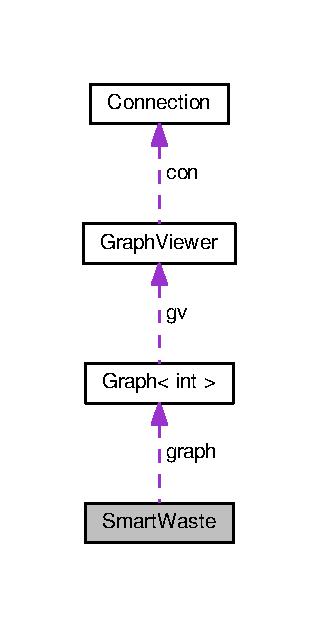
\includegraphics[width=153pt]{classSmartWaste__coll__graph}
\end{center}
\end{figure}
\subsection*{Public Member Functions}
\begin{DoxyCompactItemize}
\item 
\hyperlink{classSmartWaste_a9160cb643ea818e93ac5f129ca753372}{Smart\+Waste} (\hyperlink{classGraphViewer}{Graph\+Viewer} $\ast$gv)
\begin{DoxyCompactList}\small\item\em constructor of class \end{DoxyCompactList}\item 
void \hyperlink{classSmartWaste_ae42e3c99877f4651f931a68c34526398}{init\+Garages\+And\+Centrals} ()
\begin{DoxyCompactList}\small\item\em Generate random places for the garages and the centrals. \end{DoxyCompactList}\item 
\hyperlink{classGraph}{Graph}$<$ int $>$ $\ast$ \hyperlink{classSmartWaste_a01f8a0d4c232b6e25c8a31299cbfd3ea}{get\+Graph} ()
\begin{DoxyCompactList}\small\item\em Get the graph. \end{DoxyCompactList}\item 
void \hyperlink{classSmartWaste_a418a6bbfd147448293d26f8269a52a7a}{paint\+Nodes} (const vector$<$ int $>$ \&full\+Nodes, const string \&color)
\begin{DoxyCompactList}\small\item\em Paint all nodes of the vector. \end{DoxyCompactList}\item 
void \hyperlink{classSmartWaste_ac22248b6006d50c9a5a4c930fcdde56e}{generate\+Random\+Cases} (vector$<$ int $>$ \&full\+Nodes)
\begin{DoxyCompactList}\small\item\em Generate random test cases. \end{DoxyCompactList}\item 
void \hyperlink{classSmartWaste_aeefe2c284d3a3a83589a0a3118af0f05}{set\+Nodes\+State} (const vector$<$ int $>$ \&full\+Nodes, string color)
\begin{DoxyCompactList}\small\item\em Generate random test cases. \end{DoxyCompactList}\item 
void \hyperlink{classSmartWaste_ad794e60b6202dc3a1e38d028be2195d1}{generate\+Random\+Cases\+Recycling} (vector$<$ int $>$ \&full\+Nodes\+Paper, vector$<$ int $>$ \&full\+Nodes\+Glass, vector$<$ int $>$ \&full\+Nodes\+Plastic)
\begin{DoxyCompactList}\small\item\em Generate random test cases. \end{DoxyCompactList}\item 
int \hyperlink{classSmartWaste_a5d8ac088738eff0f301a44468e64cd1a}{compute\+Next\+Vertex} (vector$<$ int $>$ \&full\+Nodes)
\begin{DoxyCompactList}\small\item\em Return the next garbage colector to visit (closest the current souce) \end{DoxyCompactList}\item 
void \hyperlink{classSmartWaste_aa55aa107bef64f322ea140103888c40b}{add\+Path} (vector$<$ int $>$ \&path\+Solution, const vector$<$ int $>$ \&new\+Path)
\begin{DoxyCompactList}\small\item\em Add computed path so the solution. \end{DoxyCompactList}\item 
void \hyperlink{classSmartWaste_a08307d41711fbdeb0993c146201f0e39}{reset\+Node} (int current\+Node, string color)
\begin{DoxyCompactList}\small\item\em Method to reset a node or change its color if it is full of another residue. \end{DoxyCompactList}\item 
void \hyperlink{classSmartWaste_a56980331c1909fce91ff215c58e770d3}{display\+Solution} (vector$<$ int $>$ path\+Solution, unsigned int last\+Node\+Id, int truck\+Contains, string color\+Edge)
\begin{DoxyCompactList}\small\item\em Display solution. \end{DoxyCompactList}\item 
int \hyperlink{classSmartWaste_a12ed73d4cb4116b279676f0393aa6c3b}{switch\+Central\+Dikstra} () const 
\begin{DoxyCompactList}\small\item\em Choose the nearest recycling central with Dikstra algorithm. \end{DoxyCompactList}\item 
int \hyperlink{classSmartWaste_aae9728f175078ad6323c67fb0b0afce0}{switch\+Garage\+Dikstra} (const vector$<$ int $>$ \&full\+Nodes)
\begin{DoxyCompactList}\small\item\em Choose the closest garage of trucks depending on the full containers with Dikstra algorithm. \end{DoxyCompactList}\item 
void \hyperlink{classSmartWaste_ac97fb07911f6728e6d8593daa5699188}{compute\+Solution\+Dikstra} (vector$<$ int $>$ \&full\+Nodes, string color\+Edge)
\begin{DoxyCompactList}\small\item\em main of compute solution with Dikstra algorithm \end{DoxyCompactList}\item 
void \hyperlink{classSmartWaste_a633d96a03ef0aa2252d6f5fb104af863}{compute\+Solution\+Recycling} (vector$<$ int $>$ \&full\+Nodes\+Paper, vector$<$ int $>$ \&full\+Nodes\+Glass, vector$<$ int $>$ \&full\+Nodes\+Plastic)
\begin{DoxyCompactList}\small\item\em Chooses which algorithm will be used, sending the vectors of the nodes according to the type of waste. \end{DoxyCompactList}\item 
void \hyperlink{classSmartWaste_a9d2f0d30f5162dca774e5138b71d5130}{reset\+Display} ()
\begin{DoxyCompactList}\small\item\em clear the display \end{DoxyCompactList}\item 
void \hyperlink{classSmartWaste_a4b2e5cf812f4fcb7ffffabbd507f4e2e}{reset\+Graph} (vector$<$ int $>$ \&full\+Nodes, vector$<$ int $>$ \&full\+Nodes\+Paper, vector$<$ int $>$ \&full\+Nodes\+Glass, vector$<$ int $>$ \&full\+Nodes\+Plastic)
\begin{DoxyCompactList}\small\item\em clear the display and reset variables for new tests \end{DoxyCompactList}\item 
void \hyperlink{classSmartWaste_ad13fe762051a627f7c91e18b56b5871c}{paint\+Nodes} (vector$<$ int $>$ nodes, int source)
\begin{DoxyCompactList}\small\item\em Auxiliary method of analyze the connectivity of the graph. \end{DoxyCompactList}\item 
void \hyperlink{classSmartWaste_adc740c52afb954d4781555c2a24b095f}{verify\+Connectivity} ()
\begin{DoxyCompactList}\small\item\em Analyze and displays the connectivity of the graph. \end{DoxyCompactList}\item 
void \hyperlink{classSmartWaste_a8b92a14b2fc83e86d9fa797dec00ae0e}{aux\+Time\+Comparison\+Dijkstra} (vector$<$ int $>$ full\+Nodes)
\begin{DoxyCompactList}\small\item\em Auxiliary method of analyze time of Dikstra algorithm. \end{DoxyCompactList}\item 
int \hyperlink{classSmartWaste_a69c3a37338ea2c3c49b3e600d45a7afa}{switch\+Central\+Floyd\+Warshall} (int source\+Id)
\begin{DoxyCompactList}\small\item\em Choose the nearest recycling central with Floyd Warshall algorithm. \end{DoxyCompactList}\item 
int \hyperlink{classSmartWaste_a3440495b88d51595261af349753c3b4e}{switch\+Garage\+Floyd\+Warshall} (const vector$<$ int $>$ \&full\+Nodes)
\begin{DoxyCompactList}\small\item\em Choose the closest garage of trucks depending on the full containers with Floyd Warshall algorithm. \end{DoxyCompactList}\item 
void \hyperlink{classSmartWaste_a0cd6a174d186a2cf5e4d4de10df0b48c}{aux\+Time\+Comparison\+Floyd\+Warshal} (vector$<$ int $>$ full\+Nodes)
\begin{DoxyCompactList}\small\item\em Auxiliary method of analyze time of Floyd Warshall algorithm. \end{DoxyCompactList}\item 
void \hyperlink{classSmartWaste_a9afdadb947d0c2fcb979e3470c4e2721}{time\+Comparison} ()
\begin{DoxyCompactList}\small\item\em Method to compare execution times of the Floyd Warshall and the Dikstra algorithm. \end{DoxyCompactList}\item 
vector$<$ int $>$ \hyperlink{classSmartWaste_ad697e11bb3f1bb7524f939f90a6fbe9c}{exact\+Search\+Kmp} (map$<$ string, int $>$ roads\+Id\+Map, string expression)
\begin{DoxyCompactList}\small\item\em Separates each street from the map to be processed the exact search through the kmp algorithm. \end{DoxyCompactList}\item 
vector$<$ int $>$ \hyperlink{classSmartWaste_aca7293f5975100c00c7b915354520af5}{exact\+Search\+Naive} (map$<$ string, int $>$ roads\+Id\+Map, string expression)
\begin{DoxyCompactList}\small\item\em Separates each street from the map to be processed the exact search through the naive algorithm. \end{DoxyCompactList}\item 
vector$<$ int $>$ \hyperlink{classSmartWaste_a72bb77116d7a8bccb121172c27a3cd9c}{approximate\+Search} (map$<$ string, int $>$ roads\+Id\+Map, string expression)
\begin{DoxyCompactList}\small\item\em Separates each street from the map to be processed the approximate search. \end{DoxyCompactList}\item 
int \hyperlink{classSmartWaste_aaa2ba41023879d615dd60fb52126d213}{choose\+Node\+To\+Full} (int id\+Edge)
\begin{DoxyCompactList}\small\item\em Choose the node through the edge id. \end{DoxyCompactList}\item 
void \hyperlink{classSmartWaste_aa78c4f2e275c9fc4d1735900f88c4fda}{street\+Search} (map$<$ string, int $>$ roads\+Id\+Map, vector$<$ int $>$ \&full\+Nodes)
\begin{DoxyCompactList}\small\item\em main function of street search \end{DoxyCompactList}\item 
int \hyperlink{classSmartWaste_a77a8207530b931703036025cea8092a4}{choose\+Street} (vector$<$ int $>$ search\+Results)
\begin{DoxyCompactList}\small\item\em Choose the street through the search\+: first with the exact search and then with the approximate search. \end{DoxyCompactList}\item 
void \hyperlink{classSmartWaste_a5317d1e3b89416d622435be6100e0faf}{color\+Street} (int edge\+Id)
\begin{DoxyCompactList}\small\item\em color the edge \end{DoxyCompactList}\item 
void \hyperlink{classSmartWaste_ac4ab9e2882b20d1e99bf4f6b8388a811}{reset\+Edge\+Street} (int edge\+Id)
\begin{DoxyCompactList}\small\item\em reset color of the edge \end{DoxyCompactList}\item 
void \hyperlink{classSmartWaste_ac24caa86ac0a9308daf839b66ddc28ae}{time\+Comparison\+Exact\+Search} (map$<$ string, int $>$ roads\+Id\+Map)
\begin{DoxyCompactList}\small\item\em main function of comparison time in string search. \end{DoxyCompactList}\item 
void \hyperlink{classSmartWaste_a6d8bfbc9102640c3ec1e9e9d71338b30}{time\+Comparison\+K\+M\+P\+Strings\+Sizes} (map$<$ string, int $>$ roads\+Id\+Map)
\begin{DoxyCompactList}\small\item\em Calculates and displays the search time of the kmp algorithm with expressions of different sizes. \end{DoxyCompactList}\item 
void \hyperlink{classSmartWaste_a6eb1a1ed26014c2785bd880696106688}{time\+Comparison\+Naive\+Strings\+Sizes} (map$<$ string, int $>$ roads\+Id\+Map)
\begin{DoxyCompactList}\small\item\em Calculates and displays the search time of the naive algorithm with expressions of different sizes. \end{DoxyCompactList}\item 
void \hyperlink{classSmartWaste_a63d659670d34638ada6460912e6b1f8a}{time\+Comparison\+K\+M\+P\+Files\+Sizes} ()
\begin{DoxyCompactList}\small\item\em Calculates and displays the search time of the kmp algorithm on files of different sizes. \end{DoxyCompactList}\item 
void \hyperlink{classSmartWaste_a102f65c9cd8af166e72a25de85ecc467}{time\+Comparison\+Naive\+Files\+Sizes} ()
\begin{DoxyCompactList}\small\item\em Calculates and displays the search time of the naive algorithm on files of different sizes. \end{DoxyCompactList}\end{DoxyCompactItemize}
\subsection*{Private Attributes}
\begin{DoxyCompactItemize}
\item 
\hyperlink{classGraph}{Graph}$<$ int $>$ \hyperlink{classSmartWaste_a653f3e0a3fb2148fb3e59ec9532f6d04}{graph}
\item 
vector$<$ int $>$ \hyperlink{classSmartWaste_aac31f2b8c6bd3f931346024435e36f5f}{centrals}
\item 
vector$<$ int $>$ \hyperlink{classSmartWaste_a624a2893edb7c0e00e4fefe635a0c597}{garages}
\end{DoxyCompactItemize}


\subsection{Constructor \& Destructor Documentation}
\index{Smart\+Waste@{Smart\+Waste}!Smart\+Waste@{Smart\+Waste}}
\index{Smart\+Waste@{Smart\+Waste}!Smart\+Waste@{Smart\+Waste}}
\subsubsection[{\texorpdfstring{Smart\+Waste(\+Graph\+Viewer $\ast$gv)}{SmartWaste(GraphViewer *gv)}}]{\setlength{\rightskip}{0pt plus 5cm}Smart\+Waste\+::\+Smart\+Waste (
\begin{DoxyParamCaption}
\item[{{\bf Graph\+Viewer} $\ast$}]{gv}
\end{DoxyParamCaption}
)}\hypertarget{classSmartWaste_a9160cb643ea818e93ac5f129ca753372}{}\label{classSmartWaste_a9160cb643ea818e93ac5f129ca753372}


constructor of class 

F\+I\+R\+ST P\+A\+RT OF P\+R\+O\+J\+E\+CT 
\begin{DoxyParams}{Parameters}
{\em gv} & \+: graph viewer for the display \\
\hline
\end{DoxyParams}


\subsection{Member Function Documentation}
\index{Smart\+Waste@{Smart\+Waste}!add\+Path@{add\+Path}}
\index{add\+Path@{add\+Path}!Smart\+Waste@{Smart\+Waste}}
\subsubsection[{\texorpdfstring{add\+Path(vector$<$ int $>$ \&path\+Solution, const vector$<$ int $>$ \&new\+Path)}{addPath(vector< int > &pathSolution, const vector< int > &newPath)}}]{\setlength{\rightskip}{0pt plus 5cm}void Smart\+Waste\+::add\+Path (
\begin{DoxyParamCaption}
\item[{vector$<$ int $>$ \&}]{path\+Solution, }
\item[{const vector$<$ int $>$ \&}]{new\+Path}
\end{DoxyParamCaption}
)}\hypertarget{classSmartWaste_aa55aa107bef64f322ea140103888c40b}{}\label{classSmartWaste_aa55aa107bef64f322ea140103888c40b}


Add computed path so the solution. 


\begin{DoxyParams}{Parameters}
{\em path\+Solution} & \+: path solution already computed \\
\hline
{\em new\+Path} & \+: new part of the path to add \\
\hline
\end{DoxyParams}
\index{Smart\+Waste@{Smart\+Waste}!approximate\+Search@{approximate\+Search}}
\index{approximate\+Search@{approximate\+Search}!Smart\+Waste@{Smart\+Waste}}
\subsubsection[{\texorpdfstring{approximate\+Search(map$<$ string, int $>$ roads\+Id\+Map, string expression)}{approximateSearch(map< string, int > roadsIdMap, string expression)}}]{\setlength{\rightskip}{0pt plus 5cm}vector$<$ int $>$ Smart\+Waste\+::approximate\+Search (
\begin{DoxyParamCaption}
\item[{map$<$ string, int $>$}]{roads\+Id\+Map, }
\item[{string}]{expression}
\end{DoxyParamCaption}
)}\hypertarget{classSmartWaste_a72bb77116d7a8bccb121172c27a3cd9c}{}\label{classSmartWaste_a72bb77116d7a8bccb121172c27a3cd9c}


Separates each street from the map to be processed the approximate search. 


\begin{DoxyParams}{Parameters}
{\em roads\+Id\+Map} & -\/ map containing all the streets in the graph \\
\hline
{\em expression} & to search \\
\hline
\end{DoxyParams}
\begin{DoxyReturn}{Returns}
vector of results 
\end{DoxyReturn}


Here is the call graph for this function\+:
\nopagebreak
\begin{figure}[H]
\begin{center}
\leavevmode
\includegraphics[width=350pt]{classSmartWaste_a72bb77116d7a8bccb121172c27a3cd9c_cgraph}
\end{center}
\end{figure}


\index{Smart\+Waste@{Smart\+Waste}!aux\+Time\+Comparison\+Dijkstra@{aux\+Time\+Comparison\+Dijkstra}}
\index{aux\+Time\+Comparison\+Dijkstra@{aux\+Time\+Comparison\+Dijkstra}!Smart\+Waste@{Smart\+Waste}}
\subsubsection[{\texorpdfstring{aux\+Time\+Comparison\+Dijkstra(vector$<$ int $>$ full\+Nodes)}{auxTimeComparisonDijkstra(vector< int > fullNodes)}}]{\setlength{\rightskip}{0pt plus 5cm}void Smart\+Waste\+::aux\+Time\+Comparison\+Dijkstra (
\begin{DoxyParamCaption}
\item[{vector$<$ int $>$}]{full\+Nodes}
\end{DoxyParamCaption}
)}\hypertarget{classSmartWaste_a8b92a14b2fc83e86d9fa797dec00ae0e}{}\label{classSmartWaste_a8b92a14b2fc83e86d9fa797dec00ae0e}


Auxiliary method of analyze time of Dikstra algorithm. 


\begin{DoxyParams}{Parameters}
{\em full\+Nodes} & \\
\hline
\end{DoxyParams}


Here is the call graph for this function\+:
\nopagebreak
\begin{figure}[H]
\begin{center}
\leavevmode
\includegraphics[width=350pt]{classSmartWaste_a8b92a14b2fc83e86d9fa797dec00ae0e_cgraph}
\end{center}
\end{figure}


\index{Smart\+Waste@{Smart\+Waste}!aux\+Time\+Comparison\+Floyd\+Warshal@{aux\+Time\+Comparison\+Floyd\+Warshal}}
\index{aux\+Time\+Comparison\+Floyd\+Warshal@{aux\+Time\+Comparison\+Floyd\+Warshal}!Smart\+Waste@{Smart\+Waste}}
\subsubsection[{\texorpdfstring{aux\+Time\+Comparison\+Floyd\+Warshal(vector$<$ int $>$ full\+Nodes)}{auxTimeComparisonFloydWarshal(vector< int > fullNodes)}}]{\setlength{\rightskip}{0pt plus 5cm}void Smart\+Waste\+::aux\+Time\+Comparison\+Floyd\+Warshal (
\begin{DoxyParamCaption}
\item[{vector$<$ int $>$}]{full\+Nodes}
\end{DoxyParamCaption}
)}\hypertarget{classSmartWaste_a0cd6a174d186a2cf5e4d4de10df0b48c}{}\label{classSmartWaste_a0cd6a174d186a2cf5e4d4de10df0b48c}


Auxiliary method of analyze time of Floyd Warshall algorithm. 


\begin{DoxyParams}{Parameters}
{\em full\+Nodes} & \\
\hline
\end{DoxyParams}


Here is the call graph for this function\+:
\nopagebreak
\begin{figure}[H]
\begin{center}
\leavevmode
\includegraphics[width=350pt]{classSmartWaste_a0cd6a174d186a2cf5e4d4de10df0b48c_cgraph}
\end{center}
\end{figure}


\index{Smart\+Waste@{Smart\+Waste}!choose\+Node\+To\+Full@{choose\+Node\+To\+Full}}
\index{choose\+Node\+To\+Full@{choose\+Node\+To\+Full}!Smart\+Waste@{Smart\+Waste}}
\subsubsection[{\texorpdfstring{choose\+Node\+To\+Full(int id\+Edge)}{chooseNodeToFull(int idEdge)}}]{\setlength{\rightskip}{0pt plus 5cm}int Smart\+Waste\+::choose\+Node\+To\+Full (
\begin{DoxyParamCaption}
\item[{int}]{id\+Edge}
\end{DoxyParamCaption}
)}\hypertarget{classSmartWaste_aaa2ba41023879d615dd60fb52126d213}{}\label{classSmartWaste_aaa2ba41023879d615dd60fb52126d213}


Choose the node through the edge id. 


\begin{DoxyParams}{Parameters}
{\em id\+Edge} & \\
\hline
\end{DoxyParams}
\begin{DoxyReturn}{Returns}
id of the chosen node 
\end{DoxyReturn}


Here is the call graph for this function\+:
\nopagebreak
\begin{figure}[H]
\begin{center}
\leavevmode
\includegraphics[width=350pt]{classSmartWaste_aaa2ba41023879d615dd60fb52126d213_cgraph}
\end{center}
\end{figure}


\index{Smart\+Waste@{Smart\+Waste}!choose\+Street@{choose\+Street}}
\index{choose\+Street@{choose\+Street}!Smart\+Waste@{Smart\+Waste}}
\subsubsection[{\texorpdfstring{choose\+Street(vector$<$ int $>$ search\+Results)}{chooseStreet(vector< int > searchResults)}}]{\setlength{\rightskip}{0pt plus 5cm}int Smart\+Waste\+::choose\+Street (
\begin{DoxyParamCaption}
\item[{vector$<$ int $>$}]{search\+Results}
\end{DoxyParamCaption}
)}\hypertarget{classSmartWaste_a77a8207530b931703036025cea8092a4}{}\label{classSmartWaste_a77a8207530b931703036025cea8092a4}


Choose the street through the search\+: first with the exact search and then with the approximate search. 


\begin{DoxyParams}{Parameters}
{\em all} & search results \\
\hline
\end{DoxyParams}
\begin{DoxyReturn}{Returns}
id of the edge choosen (the street) 
\end{DoxyReturn}


Here is the call graph for this function\+:
\nopagebreak
\begin{figure}[H]
\begin{center}
\leavevmode
\includegraphics[width=350pt]{classSmartWaste_a77a8207530b931703036025cea8092a4_cgraph}
\end{center}
\end{figure}


\index{Smart\+Waste@{Smart\+Waste}!color\+Street@{color\+Street}}
\index{color\+Street@{color\+Street}!Smart\+Waste@{Smart\+Waste}}
\subsubsection[{\texorpdfstring{color\+Street(int edge\+Id)}{colorStreet(int edgeId)}}]{\setlength{\rightskip}{0pt plus 5cm}void Smart\+Waste\+::color\+Street (
\begin{DoxyParamCaption}
\item[{int}]{edge\+Id}
\end{DoxyParamCaption}
)}\hypertarget{classSmartWaste_a5317d1e3b89416d622435be6100e0faf}{}\label{classSmartWaste_a5317d1e3b89416d622435be6100e0faf}


color the edge 


\begin{DoxyParams}{Parameters}
{\em edge\+Id} & \\
\hline
\end{DoxyParams}


Here is the call graph for this function\+:
\nopagebreak
\begin{figure}[H]
\begin{center}
\leavevmode
\includegraphics[width=350pt]{classSmartWaste_a5317d1e3b89416d622435be6100e0faf_cgraph}
\end{center}
\end{figure}


\index{Smart\+Waste@{Smart\+Waste}!compute\+Next\+Vertex@{compute\+Next\+Vertex}}
\index{compute\+Next\+Vertex@{compute\+Next\+Vertex}!Smart\+Waste@{Smart\+Waste}}
\subsubsection[{\texorpdfstring{compute\+Next\+Vertex(vector$<$ int $>$ \&full\+Nodes)}{computeNextVertex(vector< int > &fullNodes)}}]{\setlength{\rightskip}{0pt plus 5cm}int Smart\+Waste\+::compute\+Next\+Vertex (
\begin{DoxyParamCaption}
\item[{vector$<$ int $>$ \&}]{full\+Nodes}
\end{DoxyParamCaption}
)}\hypertarget{classSmartWaste_a5d8ac088738eff0f301a44468e64cd1a}{}\label{classSmartWaste_a5d8ac088738eff0f301a44468e64cd1a}


Return the next garbage colector to visit (closest the current souce) 


\begin{DoxyParams}{Parameters}
{\em full\+Nodes} & \\
\hline
\end{DoxyParams}
\begin{DoxyReturn}{Returns}
index of the next node 
\end{DoxyReturn}


Here is the call graph for this function\+:
\nopagebreak
\begin{figure}[H]
\begin{center}
\leavevmode
\includegraphics[width=350pt]{classSmartWaste_a5d8ac088738eff0f301a44468e64cd1a_cgraph}
\end{center}
\end{figure}


\index{Smart\+Waste@{Smart\+Waste}!compute\+Solution\+Dikstra@{compute\+Solution\+Dikstra}}
\index{compute\+Solution\+Dikstra@{compute\+Solution\+Dikstra}!Smart\+Waste@{Smart\+Waste}}
\subsubsection[{\texorpdfstring{compute\+Solution\+Dikstra(vector$<$ int $>$ \&full\+Nodes, string color\+Edge)}{computeSolutionDikstra(vector< int > &fullNodes, string colorEdge)}}]{\setlength{\rightskip}{0pt plus 5cm}void Smart\+Waste\+::compute\+Solution\+Dikstra (
\begin{DoxyParamCaption}
\item[{vector$<$ int $>$ \&}]{full\+Nodes, }
\item[{string}]{color\+Edge}
\end{DoxyParamCaption}
)}\hypertarget{classSmartWaste_ac97fb07911f6728e6d8593daa5699188}{}\label{classSmartWaste_ac97fb07911f6728e6d8593daa5699188}


main of compute solution with Dikstra algorithm 


\begin{DoxyParams}{Parameters}
{\em full\+Nodes} & \\
\hline
{\em color} & of the edge \\
\hline
\end{DoxyParams}


Here is the call graph for this function\+:
\nopagebreak
\begin{figure}[H]
\begin{center}
\leavevmode
\includegraphics[width=350pt]{classSmartWaste_ac97fb07911f6728e6d8593daa5699188_cgraph}
\end{center}
\end{figure}


\index{Smart\+Waste@{Smart\+Waste}!compute\+Solution\+Recycling@{compute\+Solution\+Recycling}}
\index{compute\+Solution\+Recycling@{compute\+Solution\+Recycling}!Smart\+Waste@{Smart\+Waste}}
\subsubsection[{\texorpdfstring{compute\+Solution\+Recycling(vector$<$ int $>$ \&full\+Nodes\+Paper, vector$<$ int $>$ \&full\+Nodes\+Glass, vector$<$ int $>$ \&full\+Nodes\+Plastic)}{computeSolutionRecycling(vector< int > &fullNodesPaper, vector< int > &fullNodesGlass, vector< int > &fullNodesPlastic)}}]{\setlength{\rightskip}{0pt plus 5cm}void Smart\+Waste\+::compute\+Solution\+Recycling (
\begin{DoxyParamCaption}
\item[{vector$<$ int $>$ \&}]{full\+Nodes\+Paper, }
\item[{vector$<$ int $>$ \&}]{full\+Nodes\+Glass, }
\item[{vector$<$ int $>$ \&}]{full\+Nodes\+Plastic}
\end{DoxyParamCaption}
)}\hypertarget{classSmartWaste_a633d96a03ef0aa2252d6f5fb104af863}{}\label{classSmartWaste_a633d96a03ef0aa2252d6f5fb104af863}


Chooses which algorithm will be used, sending the vectors of the nodes according to the type of waste. 


\begin{DoxyParams}{Parameters}
{\em full} & nodes of paper \\
\hline
{\em full} & nodes of glass \\
\hline
{\em full} & nodes of plastic \\
\hline
\end{DoxyParams}


Here is the call graph for this function\+:
\nopagebreak
\begin{figure}[H]
\begin{center}
\leavevmode
\includegraphics[width=350pt]{classSmartWaste_a633d96a03ef0aa2252d6f5fb104af863_cgraph}
\end{center}
\end{figure}


\index{Smart\+Waste@{Smart\+Waste}!display\+Solution@{display\+Solution}}
\index{display\+Solution@{display\+Solution}!Smart\+Waste@{Smart\+Waste}}
\subsubsection[{\texorpdfstring{display\+Solution(vector$<$ int $>$ path\+Solution, unsigned int last\+Node\+Id, int truck\+Contains, string color\+Edge)}{displaySolution(vector< int > pathSolution, unsigned int lastNodeId, int truckContains, string colorEdge)}}]{\setlength{\rightskip}{0pt plus 5cm}void Smart\+Waste\+::display\+Solution (
\begin{DoxyParamCaption}
\item[{vector$<$ int $>$}]{path\+Solution, }
\item[{unsigned int}]{last\+Node\+Id, }
\item[{int}]{truck\+Contains, }
\item[{string}]{color\+Edge}
\end{DoxyParamCaption}
)}\hypertarget{classSmartWaste_a56980331c1909fce91ff215c58e770d3}{}\label{classSmartWaste_a56980331c1909fce91ff215c58e770d3}


Display solution. 


\begin{DoxyParams}{Parameters}
{\em path\+Solution} & \+: vector of path solution \\
\hline
{\em last\+Node\+Id} & \+: Auxiliary id for verify if need reset this node \\
\hline
{\em truck\+Contains} & \+: Truck contents \\
\hline
{\em color\+Edge} & \+: Color to paint the edge \\
\hline
\end{DoxyParams}


Here is the call graph for this function\+:
\nopagebreak
\begin{figure}[H]
\begin{center}
\leavevmode
\includegraphics[width=350pt]{classSmartWaste_a56980331c1909fce91ff215c58e770d3_cgraph}
\end{center}
\end{figure}


\index{Smart\+Waste@{Smart\+Waste}!exact\+Search\+Kmp@{exact\+Search\+Kmp}}
\index{exact\+Search\+Kmp@{exact\+Search\+Kmp}!Smart\+Waste@{Smart\+Waste}}
\subsubsection[{\texorpdfstring{exact\+Search\+Kmp(map$<$ string, int $>$ roads\+Id\+Map, string expression)}{exactSearchKmp(map< string, int > roadsIdMap, string expression)}}]{\setlength{\rightskip}{0pt plus 5cm}vector$<$ int $>$ Smart\+Waste\+::exact\+Search\+Kmp (
\begin{DoxyParamCaption}
\item[{map$<$ string, int $>$}]{roads\+Id\+Map, }
\item[{string}]{expression}
\end{DoxyParamCaption}
)}\hypertarget{classSmartWaste_ad697e11bb3f1bb7524f939f90a6fbe9c}{}\label{classSmartWaste_ad697e11bb3f1bb7524f939f90a6fbe9c}


Separates each street from the map to be processed the exact search through the kmp algorithm. 

S\+E\+C\+O\+ND P\+A\+RT OF P\+R\+O\+J\+E\+CT 
\begin{DoxyParams}{Parameters}
{\em roads\+Id\+Map} & -\/ map containing all the streets in the graph \\
\hline
{\em expression} & to search \\
\hline
\end{DoxyParams}
\begin{DoxyReturn}{Returns}
vector of results 
\end{DoxyReturn}


Here is the call graph for this function\+:
\nopagebreak
\begin{figure}[H]
\begin{center}
\leavevmode
\includegraphics[width=350pt]{classSmartWaste_ad697e11bb3f1bb7524f939f90a6fbe9c_cgraph}
\end{center}
\end{figure}


\index{Smart\+Waste@{Smart\+Waste}!exact\+Search\+Naive@{exact\+Search\+Naive}}
\index{exact\+Search\+Naive@{exact\+Search\+Naive}!Smart\+Waste@{Smart\+Waste}}
\subsubsection[{\texorpdfstring{exact\+Search\+Naive(map$<$ string, int $>$ roads\+Id\+Map, string expression)}{exactSearchNaive(map< string, int > roadsIdMap, string expression)}}]{\setlength{\rightskip}{0pt plus 5cm}vector$<$ int $>$ Smart\+Waste\+::exact\+Search\+Naive (
\begin{DoxyParamCaption}
\item[{map$<$ string, int $>$}]{roads\+Id\+Map, }
\item[{string}]{expression}
\end{DoxyParamCaption}
)}\hypertarget{classSmartWaste_aca7293f5975100c00c7b915354520af5}{}\label{classSmartWaste_aca7293f5975100c00c7b915354520af5}


Separates each street from the map to be processed the exact search through the naive algorithm. 


\begin{DoxyParams}{Parameters}
{\em roads\+Id\+Map} & -\/ map containing all the streets in the graph \\
\hline
{\em expression} & to search \\
\hline
\end{DoxyParams}
\begin{DoxyReturn}{Returns}
vector of results 
\end{DoxyReturn}


Here is the call graph for this function\+:
\nopagebreak
\begin{figure}[H]
\begin{center}
\leavevmode
\includegraphics[width=350pt]{classSmartWaste_aca7293f5975100c00c7b915354520af5_cgraph}
\end{center}
\end{figure}


\index{Smart\+Waste@{Smart\+Waste}!generate\+Random\+Cases@{generate\+Random\+Cases}}
\index{generate\+Random\+Cases@{generate\+Random\+Cases}!Smart\+Waste@{Smart\+Waste}}
\subsubsection[{\texorpdfstring{generate\+Random\+Cases(vector$<$ int $>$ \&full\+Nodes)}{generateRandomCases(vector< int > &fullNodes)}}]{\setlength{\rightskip}{0pt plus 5cm}void Smart\+Waste\+::generate\+Random\+Cases (
\begin{DoxyParamCaption}
\item[{vector$<$ int $>$ \&}]{full\+Nodes}
\end{DoxyParamCaption}
)}\hypertarget{classSmartWaste_ac22248b6006d50c9a5a4c930fcdde56e}{}\label{classSmartWaste_ac22248b6006d50c9a5a4c930fcdde56e}


Generate random test cases. 


\begin{DoxyParams}{Parameters}
{\em full\+Nodes} & \\
\hline
\end{DoxyParams}


Here is the call graph for this function\+:
\nopagebreak
\begin{figure}[H]
\begin{center}
\leavevmode
\includegraphics[width=350pt]{classSmartWaste_ac22248b6006d50c9a5a4c930fcdde56e_cgraph}
\end{center}
\end{figure}


\index{Smart\+Waste@{Smart\+Waste}!generate\+Random\+Cases\+Recycling@{generate\+Random\+Cases\+Recycling}}
\index{generate\+Random\+Cases\+Recycling@{generate\+Random\+Cases\+Recycling}!Smart\+Waste@{Smart\+Waste}}
\subsubsection[{\texorpdfstring{generate\+Random\+Cases\+Recycling(vector$<$ int $>$ \&full\+Nodes\+Paper, vector$<$ int $>$ \&full\+Nodes\+Glass, vector$<$ int $>$ \&full\+Nodes\+Plastic)}{generateRandomCasesRecycling(vector< int > &fullNodesPaper, vector< int > &fullNodesGlass, vector< int > &fullNodesPlastic)}}]{\setlength{\rightskip}{0pt plus 5cm}void Smart\+Waste\+::generate\+Random\+Cases\+Recycling (
\begin{DoxyParamCaption}
\item[{vector$<$ int $>$ \&}]{full\+Nodes\+Paper, }
\item[{vector$<$ int $>$ \&}]{full\+Nodes\+Glass, }
\item[{vector$<$ int $>$ \&}]{full\+Nodes\+Plastic}
\end{DoxyParamCaption}
)}\hypertarget{classSmartWaste_ad794e60b6202dc3a1e38d028be2195d1}{}\label{classSmartWaste_ad794e60b6202dc3a1e38d028be2195d1}


Generate random test cases. 


\begin{DoxyParams}{Parameters}
{\em full\+Nodes\+Glass} & \\
\hline
{\em full\+Nodes\+Paper} & \\
\hline
{\em full\+Nodes\+Plastic} & \\
\hline
\end{DoxyParams}


Here is the call graph for this function\+:
\nopagebreak
\begin{figure}[H]
\begin{center}
\leavevmode
\includegraphics[width=350pt]{classSmartWaste_ad794e60b6202dc3a1e38d028be2195d1_cgraph}
\end{center}
\end{figure}


\index{Smart\+Waste@{Smart\+Waste}!get\+Graph@{get\+Graph}}
\index{get\+Graph@{get\+Graph}!Smart\+Waste@{Smart\+Waste}}
\subsubsection[{\texorpdfstring{get\+Graph()}{getGraph()}}]{\setlength{\rightskip}{0pt plus 5cm}{\bf Graph}$<$ int $>$ $\ast$ Smart\+Waste\+::get\+Graph (
\begin{DoxyParamCaption}
{}
\end{DoxyParamCaption}
)}\hypertarget{classSmartWaste_a01f8a0d4c232b6e25c8a31299cbfd3ea}{}\label{classSmartWaste_a01f8a0d4c232b6e25c8a31299cbfd3ea}


Get the graph. 

\begin{DoxyReturn}{Returns}
the graph 
\end{DoxyReturn}
\index{Smart\+Waste@{Smart\+Waste}!init\+Garages\+And\+Centrals@{init\+Garages\+And\+Centrals}}
\index{init\+Garages\+And\+Centrals@{init\+Garages\+And\+Centrals}!Smart\+Waste@{Smart\+Waste}}
\subsubsection[{\texorpdfstring{init\+Garages\+And\+Centrals()}{initGaragesAndCentrals()}}]{\setlength{\rightskip}{0pt plus 5cm}void Smart\+Waste\+::init\+Garages\+And\+Centrals (
\begin{DoxyParamCaption}
{}
\end{DoxyParamCaption}
)}\hypertarget{classSmartWaste_ae42e3c99877f4651f931a68c34526398}{}\label{classSmartWaste_ae42e3c99877f4651f931a68c34526398}


Generate random places for the garages and the centrals. 



Here is the call graph for this function\+:
\nopagebreak
\begin{figure}[H]
\begin{center}
\leavevmode
\includegraphics[width=350pt]{classSmartWaste_ae42e3c99877f4651f931a68c34526398_cgraph}
\end{center}
\end{figure}


\index{Smart\+Waste@{Smart\+Waste}!paint\+Nodes@{paint\+Nodes}}
\index{paint\+Nodes@{paint\+Nodes}!Smart\+Waste@{Smart\+Waste}}
\subsubsection[{\texorpdfstring{paint\+Nodes(const vector$<$ int $>$ \&full\+Nodes, const string \&color)}{paintNodes(const vector< int > &fullNodes, const string &color)}}]{\setlength{\rightskip}{0pt plus 5cm}void Smart\+Waste\+::paint\+Nodes (
\begin{DoxyParamCaption}
\item[{const vector$<$ int $>$ \&}]{full\+Nodes, }
\item[{const string \&}]{color}
\end{DoxyParamCaption}
)}\hypertarget{classSmartWaste_a418a6bbfd147448293d26f8269a52a7a}{}\label{classSmartWaste_a418a6bbfd147448293d26f8269a52a7a}


Paint all nodes of the vector. 


\begin{DoxyParams}{Parameters}
{\em full\+Nodes} & \\
\hline
{\em color} & \\
\hline
\end{DoxyParams}


Here is the call graph for this function\+:
\nopagebreak
\begin{figure}[H]
\begin{center}
\leavevmode
\includegraphics[width=350pt]{classSmartWaste_a418a6bbfd147448293d26f8269a52a7a_cgraph}
\end{center}
\end{figure}


\index{Smart\+Waste@{Smart\+Waste}!paint\+Nodes@{paint\+Nodes}}
\index{paint\+Nodes@{paint\+Nodes}!Smart\+Waste@{Smart\+Waste}}
\subsubsection[{\texorpdfstring{paint\+Nodes(vector$<$ int $>$ nodes, int source)}{paintNodes(vector< int > nodes, int source)}}]{\setlength{\rightskip}{0pt plus 5cm}void Smart\+Waste\+::paint\+Nodes (
\begin{DoxyParamCaption}
\item[{vector$<$ int $>$}]{nodes, }
\item[{int}]{source}
\end{DoxyParamCaption}
)}\hypertarget{classSmartWaste_ad13fe762051a627f7c91e18b56b5871c}{}\label{classSmartWaste_ad13fe762051a627f7c91e18b56b5871c}


Auxiliary method of analyze the connectivity of the graph. 


\begin{DoxyParams}{Parameters}
{\em nodes} & \\
\hline
{\em source} & node id for init the analyze, therefore it is not to paint \\
\hline
\end{DoxyParams}


Here is the call graph for this function\+:
\nopagebreak
\begin{figure}[H]
\begin{center}
\leavevmode
\includegraphics[width=350pt]{classSmartWaste_ad13fe762051a627f7c91e18b56b5871c_cgraph}
\end{center}
\end{figure}


\index{Smart\+Waste@{Smart\+Waste}!reset\+Display@{reset\+Display}}
\index{reset\+Display@{reset\+Display}!Smart\+Waste@{Smart\+Waste}}
\subsubsection[{\texorpdfstring{reset\+Display()}{resetDisplay()}}]{\setlength{\rightskip}{0pt plus 5cm}void Smart\+Waste\+::reset\+Display (
\begin{DoxyParamCaption}
{}
\end{DoxyParamCaption}
)}\hypertarget{classSmartWaste_a9d2f0d30f5162dca774e5138b71d5130}{}\label{classSmartWaste_a9d2f0d30f5162dca774e5138b71d5130}


clear the display 



Here is the call graph for this function\+:
\nopagebreak
\begin{figure}[H]
\begin{center}
\leavevmode
\includegraphics[width=350pt]{classSmartWaste_a9d2f0d30f5162dca774e5138b71d5130_cgraph}
\end{center}
\end{figure}


\index{Smart\+Waste@{Smart\+Waste}!reset\+Edge\+Street@{reset\+Edge\+Street}}
\index{reset\+Edge\+Street@{reset\+Edge\+Street}!Smart\+Waste@{Smart\+Waste}}
\subsubsection[{\texorpdfstring{reset\+Edge\+Street(int edge\+Id)}{resetEdgeStreet(int edgeId)}}]{\setlength{\rightskip}{0pt plus 5cm}void Smart\+Waste\+::reset\+Edge\+Street (
\begin{DoxyParamCaption}
\item[{int}]{edge\+Id}
\end{DoxyParamCaption}
)}\hypertarget{classSmartWaste_ac4ab9e2882b20d1e99bf4f6b8388a811}{}\label{classSmartWaste_ac4ab9e2882b20d1e99bf4f6b8388a811}


reset color of the edge 


\begin{DoxyParams}{Parameters}
{\em edge\+Id} & \\
\hline
\end{DoxyParams}


Here is the call graph for this function\+:
\nopagebreak
\begin{figure}[H]
\begin{center}
\leavevmode
\includegraphics[width=350pt]{classSmartWaste_ac4ab9e2882b20d1e99bf4f6b8388a811_cgraph}
\end{center}
\end{figure}


\index{Smart\+Waste@{Smart\+Waste}!reset\+Graph@{reset\+Graph}}
\index{reset\+Graph@{reset\+Graph}!Smart\+Waste@{Smart\+Waste}}
\subsubsection[{\texorpdfstring{reset\+Graph(vector$<$ int $>$ \&full\+Nodes, vector$<$ int $>$ \&full\+Nodes\+Paper, vector$<$ int $>$ \&full\+Nodes\+Glass, vector$<$ int $>$ \&full\+Nodes\+Plastic)}{resetGraph(vector< int > &fullNodes, vector< int > &fullNodesPaper, vector< int > &fullNodesGlass, vector< int > &fullNodesPlastic)}}]{\setlength{\rightskip}{0pt plus 5cm}void Smart\+Waste\+::reset\+Graph (
\begin{DoxyParamCaption}
\item[{vector$<$ int $>$ \&}]{full\+Nodes, }
\item[{vector$<$ int $>$ \&}]{full\+Nodes\+Paper, }
\item[{vector$<$ int $>$ \&}]{full\+Nodes\+Glass, }
\item[{vector$<$ int $>$ \&}]{full\+Nodes\+Plastic}
\end{DoxyParamCaption}
)}\hypertarget{classSmartWaste_a4b2e5cf812f4fcb7ffffabbd507f4e2e}{}\label{classSmartWaste_a4b2e5cf812f4fcb7ffffabbd507f4e2e}


clear the display and reset variables for new tests 


\begin{DoxyParams}{Parameters}
{\em full\+Nodes} & \\
\hline
{\em full\+Nodes\+Paper} & \\
\hline
{\em full\+Nodes\+Glass} & \\
\hline
{\em full\+Nodes\+Plastic} & \\
\hline
\end{DoxyParams}


Here is the call graph for this function\+:
\nopagebreak
\begin{figure}[H]
\begin{center}
\leavevmode
\includegraphics[width=350pt]{classSmartWaste_a4b2e5cf812f4fcb7ffffabbd507f4e2e_cgraph}
\end{center}
\end{figure}


\index{Smart\+Waste@{Smart\+Waste}!reset\+Node@{reset\+Node}}
\index{reset\+Node@{reset\+Node}!Smart\+Waste@{Smart\+Waste}}
\subsubsection[{\texorpdfstring{reset\+Node(int current\+Node, string color)}{resetNode(int currentNode, string color)}}]{\setlength{\rightskip}{0pt plus 5cm}void Smart\+Waste\+::reset\+Node (
\begin{DoxyParamCaption}
\item[{int}]{current\+Node, }
\item[{string}]{color}
\end{DoxyParamCaption}
)}\hypertarget{classSmartWaste_a08307d41711fbdeb0993c146201f0e39}{}\label{classSmartWaste_a08307d41711fbdeb0993c146201f0e39}


Method to reset a node or change its color if it is full of another residue. 


\begin{DoxyParams}{Parameters}
{\em current\+Node} & \+: current node id \\
\hline
{\em color} & current color of this node \\
\hline
\end{DoxyParams}


Here is the call graph for this function\+:
\nopagebreak
\begin{figure}[H]
\begin{center}
\leavevmode
\includegraphics[width=350pt]{classSmartWaste_a08307d41711fbdeb0993c146201f0e39_cgraph}
\end{center}
\end{figure}


\index{Smart\+Waste@{Smart\+Waste}!set\+Nodes\+State@{set\+Nodes\+State}}
\index{set\+Nodes\+State@{set\+Nodes\+State}!Smart\+Waste@{Smart\+Waste}}
\subsubsection[{\texorpdfstring{set\+Nodes\+State(const vector$<$ int $>$ \&full\+Nodes, string color)}{setNodesState(const vector< int > &fullNodes, string color)}}]{\setlength{\rightskip}{0pt plus 5cm}void Smart\+Waste\+::set\+Nodes\+State (
\begin{DoxyParamCaption}
\item[{const vector$<$ int $>$ \&}]{full\+Nodes, }
\item[{string}]{color}
\end{DoxyParamCaption}
)}\hypertarget{classSmartWaste_aeefe2c284d3a3a83589a0a3118af0f05}{}\label{classSmartWaste_aeefe2c284d3a3a83589a0a3118af0f05}


Generate random test cases. 


\begin{DoxyParams}{Parameters}
{\em full\+Nodes} & \\
\hline
{\em color} & \\
\hline
\end{DoxyParams}


Here is the call graph for this function\+:
\nopagebreak
\begin{figure}[H]
\begin{center}
\leavevmode
\includegraphics[width=350pt]{classSmartWaste_aeefe2c284d3a3a83589a0a3118af0f05_cgraph}
\end{center}
\end{figure}


\index{Smart\+Waste@{Smart\+Waste}!street\+Search@{street\+Search}}
\index{street\+Search@{street\+Search}!Smart\+Waste@{Smart\+Waste}}
\subsubsection[{\texorpdfstring{street\+Search(map$<$ string, int $>$ roads\+Id\+Map, vector$<$ int $>$ \&full\+Nodes)}{streetSearch(map< string, int > roadsIdMap, vector< int > &fullNodes)}}]{\setlength{\rightskip}{0pt plus 5cm}void Smart\+Waste\+::street\+Search (
\begin{DoxyParamCaption}
\item[{map$<$ string, int $>$}]{roads\+Id\+Map, }
\item[{vector$<$ int $>$ \&}]{full\+Nodes}
\end{DoxyParamCaption}
)}\hypertarget{classSmartWaste_aa78c4f2e275c9fc4d1735900f88c4fda}{}\label{classSmartWaste_aa78c4f2e275c9fc4d1735900f88c4fda}


main function of street search 


\begin{DoxyParams}{Parameters}
{\em roads\+Id\+Map} & -\/ map containing all the streets in the graph \\
\hline
{\em full\+Nodes} & -\/ vector of nodes to signal as full \\
\hline
\end{DoxyParams}


Here is the call graph for this function\+:
\nopagebreak
\begin{figure}[H]
\begin{center}
\leavevmode
\includegraphics[width=350pt]{classSmartWaste_aa78c4f2e275c9fc4d1735900f88c4fda_cgraph}
\end{center}
\end{figure}


\index{Smart\+Waste@{Smart\+Waste}!switch\+Central\+Dikstra@{switch\+Central\+Dikstra}}
\index{switch\+Central\+Dikstra@{switch\+Central\+Dikstra}!Smart\+Waste@{Smart\+Waste}}
\subsubsection[{\texorpdfstring{switch\+Central\+Dikstra() const }{switchCentralDikstra() const }}]{\setlength{\rightskip}{0pt plus 5cm}int Smart\+Waste\+::switch\+Central\+Dikstra (
\begin{DoxyParamCaption}
{}
\end{DoxyParamCaption}
) const}\hypertarget{classSmartWaste_a12ed73d4cb4116b279676f0393aa6c3b}{}\label{classSmartWaste_a12ed73d4cb4116b279676f0393aa6c3b}


Choose the nearest recycling central with Dikstra algorithm. 

\begin{DoxyReturn}{Returns}
central node id 
\end{DoxyReturn}


Here is the call graph for this function\+:
\nopagebreak
\begin{figure}[H]
\begin{center}
\leavevmode
\includegraphics[width=344pt]{classSmartWaste_a12ed73d4cb4116b279676f0393aa6c3b_cgraph}
\end{center}
\end{figure}


\index{Smart\+Waste@{Smart\+Waste}!switch\+Central\+Floyd\+Warshall@{switch\+Central\+Floyd\+Warshall}}
\index{switch\+Central\+Floyd\+Warshall@{switch\+Central\+Floyd\+Warshall}!Smart\+Waste@{Smart\+Waste}}
\subsubsection[{\texorpdfstring{switch\+Central\+Floyd\+Warshall(int source\+Id)}{switchCentralFloydWarshall(int sourceId)}}]{\setlength{\rightskip}{0pt plus 5cm}int Smart\+Waste\+::switch\+Central\+Floyd\+Warshall (
\begin{DoxyParamCaption}
\item[{int}]{source\+Id}
\end{DoxyParamCaption}
)}\hypertarget{classSmartWaste_a69c3a37338ea2c3c49b3e600d45a7afa}{}\label{classSmartWaste_a69c3a37338ea2c3c49b3e600d45a7afa}


Choose the nearest recycling central with Floyd Warshall algorithm. 


\begin{DoxyParams}{Parameters}
{\em source\+Id} & \\
\hline
\end{DoxyParams}
\begin{DoxyReturn}{Returns}
central node id 
\end{DoxyReturn}


Here is the call graph for this function\+:
\nopagebreak
\begin{figure}[H]
\begin{center}
\leavevmode
\includegraphics[width=350pt]{classSmartWaste_a69c3a37338ea2c3c49b3e600d45a7afa_cgraph}
\end{center}
\end{figure}


\index{Smart\+Waste@{Smart\+Waste}!switch\+Garage\+Dikstra@{switch\+Garage\+Dikstra}}
\index{switch\+Garage\+Dikstra@{switch\+Garage\+Dikstra}!Smart\+Waste@{Smart\+Waste}}
\subsubsection[{\texorpdfstring{switch\+Garage\+Dikstra(const vector$<$ int $>$ \&full\+Nodes)}{switchGarageDikstra(const vector< int > &fullNodes)}}]{\setlength{\rightskip}{0pt plus 5cm}int Smart\+Waste\+::switch\+Garage\+Dikstra (
\begin{DoxyParamCaption}
\item[{const vector$<$ int $>$ \&}]{full\+Nodes}
\end{DoxyParamCaption}
)}\hypertarget{classSmartWaste_aae9728f175078ad6323c67fb0b0afce0}{}\label{classSmartWaste_aae9728f175078ad6323c67fb0b0afce0}


Choose the closest garage of trucks depending on the full containers with Dikstra algorithm. 


\begin{DoxyParams}{Parameters}
{\em full\+Nodes} & \\
\hline
\end{DoxyParams}
\begin{DoxyReturn}{Returns}
garage node id 
\end{DoxyReturn}


Here is the call graph for this function\+:
\nopagebreak
\begin{figure}[H]
\begin{center}
\leavevmode
\includegraphics[width=350pt]{classSmartWaste_aae9728f175078ad6323c67fb0b0afce0_cgraph}
\end{center}
\end{figure}


\index{Smart\+Waste@{Smart\+Waste}!switch\+Garage\+Floyd\+Warshall@{switch\+Garage\+Floyd\+Warshall}}
\index{switch\+Garage\+Floyd\+Warshall@{switch\+Garage\+Floyd\+Warshall}!Smart\+Waste@{Smart\+Waste}}
\subsubsection[{\texorpdfstring{switch\+Garage\+Floyd\+Warshall(const vector$<$ int $>$ \&full\+Nodes)}{switchGarageFloydWarshall(const vector< int > &fullNodes)}}]{\setlength{\rightskip}{0pt plus 5cm}int Smart\+Waste\+::switch\+Garage\+Floyd\+Warshall (
\begin{DoxyParamCaption}
\item[{const vector$<$ int $>$ \&}]{full\+Nodes}
\end{DoxyParamCaption}
)}\hypertarget{classSmartWaste_a3440495b88d51595261af349753c3b4e}{}\label{classSmartWaste_a3440495b88d51595261af349753c3b4e}


Choose the closest garage of trucks depending on the full containers with Floyd Warshall algorithm. 


\begin{DoxyParams}{Parameters}
{\em full\+Nodes} & \\
\hline
\end{DoxyParams}
\begin{DoxyReturn}{Returns}
garage node id 
\end{DoxyReturn}


Here is the call graph for this function\+:
\nopagebreak
\begin{figure}[H]
\begin{center}
\leavevmode
\includegraphics[width=350pt]{classSmartWaste_a3440495b88d51595261af349753c3b4e_cgraph}
\end{center}
\end{figure}


\index{Smart\+Waste@{Smart\+Waste}!time\+Comparison@{time\+Comparison}}
\index{time\+Comparison@{time\+Comparison}!Smart\+Waste@{Smart\+Waste}}
\subsubsection[{\texorpdfstring{time\+Comparison()}{timeComparison()}}]{\setlength{\rightskip}{0pt plus 5cm}void Smart\+Waste\+::time\+Comparison (
\begin{DoxyParamCaption}
{}
\end{DoxyParamCaption}
)}\hypertarget{classSmartWaste_a9afdadb947d0c2fcb979e3470c4e2721}{}\label{classSmartWaste_a9afdadb947d0c2fcb979e3470c4e2721}


Method to compare execution times of the Floyd Warshall and the Dikstra algorithm. 



Here is the call graph for this function\+:
\nopagebreak
\begin{figure}[H]
\begin{center}
\leavevmode
\includegraphics[width=350pt]{classSmartWaste_a9afdadb947d0c2fcb979e3470c4e2721_cgraph}
\end{center}
\end{figure}


\index{Smart\+Waste@{Smart\+Waste}!time\+Comparison\+Exact\+Search@{time\+Comparison\+Exact\+Search}}
\index{time\+Comparison\+Exact\+Search@{time\+Comparison\+Exact\+Search}!Smart\+Waste@{Smart\+Waste}}
\subsubsection[{\texorpdfstring{time\+Comparison\+Exact\+Search(map$<$ string, int $>$ roads\+Id\+Map)}{timeComparisonExactSearch(map< string, int > roadsIdMap)}}]{\setlength{\rightskip}{0pt plus 5cm}void Smart\+Waste\+::time\+Comparison\+Exact\+Search (
\begin{DoxyParamCaption}
\item[{map$<$ string, int $>$}]{roads\+Id\+Map}
\end{DoxyParamCaption}
)}\hypertarget{classSmartWaste_ac24caa86ac0a9308daf839b66ddc28ae}{}\label{classSmartWaste_ac24caa86ac0a9308daf839b66ddc28ae}


main function of comparison time in string search. 


\begin{DoxyParams}{Parameters}
{\em full\+Nodes} & \\
\hline
\end{DoxyParams}


Here is the call graph for this function\+:
\nopagebreak
\begin{figure}[H]
\begin{center}
\leavevmode
\includegraphics[width=350pt]{classSmartWaste_ac24caa86ac0a9308daf839b66ddc28ae_cgraph}
\end{center}
\end{figure}


\index{Smart\+Waste@{Smart\+Waste}!time\+Comparison\+K\+M\+P\+Files\+Sizes@{time\+Comparison\+K\+M\+P\+Files\+Sizes}}
\index{time\+Comparison\+K\+M\+P\+Files\+Sizes@{time\+Comparison\+K\+M\+P\+Files\+Sizes}!Smart\+Waste@{Smart\+Waste}}
\subsubsection[{\texorpdfstring{time\+Comparison\+K\+M\+P\+Files\+Sizes()}{timeComparisonKMPFilesSizes()}}]{\setlength{\rightskip}{0pt plus 5cm}void Smart\+Waste\+::time\+Comparison\+K\+M\+P\+Files\+Sizes (
\begin{DoxyParamCaption}
{}
\end{DoxyParamCaption}
)}\hypertarget{classSmartWaste_a63d659670d34638ada6460912e6b1f8a}{}\label{classSmartWaste_a63d659670d34638ada6460912e6b1f8a}


Calculates and displays the search time of the kmp algorithm on files of different sizes. 



Here is the call graph for this function\+:
\nopagebreak
\begin{figure}[H]
\begin{center}
\leavevmode
\includegraphics[width=350pt]{classSmartWaste_a63d659670d34638ada6460912e6b1f8a_cgraph}
\end{center}
\end{figure}


\index{Smart\+Waste@{Smart\+Waste}!time\+Comparison\+K\+M\+P\+Strings\+Sizes@{time\+Comparison\+K\+M\+P\+Strings\+Sizes}}
\index{time\+Comparison\+K\+M\+P\+Strings\+Sizes@{time\+Comparison\+K\+M\+P\+Strings\+Sizes}!Smart\+Waste@{Smart\+Waste}}
\subsubsection[{\texorpdfstring{time\+Comparison\+K\+M\+P\+Strings\+Sizes(map$<$ string, int $>$ roads\+Id\+Map)}{timeComparisonKMPStringsSizes(map< string, int > roadsIdMap)}}]{\setlength{\rightskip}{0pt plus 5cm}void Smart\+Waste\+::time\+Comparison\+K\+M\+P\+Strings\+Sizes (
\begin{DoxyParamCaption}
\item[{map$<$ string, int $>$}]{roads\+Id\+Map}
\end{DoxyParamCaption}
)}\hypertarget{classSmartWaste_a6d8bfbc9102640c3ec1e9e9d71338b30}{}\label{classSmartWaste_a6d8bfbc9102640c3ec1e9e9d71338b30}


Calculates and displays the search time of the kmp algorithm with expressions of different sizes. 


\begin{DoxyParams}{Parameters}
{\em full\+Nodes} & \\
\hline
\end{DoxyParams}


Here is the call graph for this function\+:
\nopagebreak
\begin{figure}[H]
\begin{center}
\leavevmode
\includegraphics[width=350pt]{classSmartWaste_a6d8bfbc9102640c3ec1e9e9d71338b30_cgraph}
\end{center}
\end{figure}


\index{Smart\+Waste@{Smart\+Waste}!time\+Comparison\+Naive\+Files\+Sizes@{time\+Comparison\+Naive\+Files\+Sizes}}
\index{time\+Comparison\+Naive\+Files\+Sizes@{time\+Comparison\+Naive\+Files\+Sizes}!Smart\+Waste@{Smart\+Waste}}
\subsubsection[{\texorpdfstring{time\+Comparison\+Naive\+Files\+Sizes()}{timeComparisonNaiveFilesSizes()}}]{\setlength{\rightskip}{0pt plus 5cm}void Smart\+Waste\+::time\+Comparison\+Naive\+Files\+Sizes (
\begin{DoxyParamCaption}
{}
\end{DoxyParamCaption}
)}\hypertarget{classSmartWaste_a102f65c9cd8af166e72a25de85ecc467}{}\label{classSmartWaste_a102f65c9cd8af166e72a25de85ecc467}


Calculates and displays the search time of the naive algorithm on files of different sizes. 



Here is the call graph for this function\+:
\nopagebreak
\begin{figure}[H]
\begin{center}
\leavevmode
\includegraphics[width=350pt]{classSmartWaste_a102f65c9cd8af166e72a25de85ecc467_cgraph}
\end{center}
\end{figure}


\index{Smart\+Waste@{Smart\+Waste}!time\+Comparison\+Naive\+Strings\+Sizes@{time\+Comparison\+Naive\+Strings\+Sizes}}
\index{time\+Comparison\+Naive\+Strings\+Sizes@{time\+Comparison\+Naive\+Strings\+Sizes}!Smart\+Waste@{Smart\+Waste}}
\subsubsection[{\texorpdfstring{time\+Comparison\+Naive\+Strings\+Sizes(map$<$ string, int $>$ roads\+Id\+Map)}{timeComparisonNaiveStringsSizes(map< string, int > roadsIdMap)}}]{\setlength{\rightskip}{0pt plus 5cm}void Smart\+Waste\+::time\+Comparison\+Naive\+Strings\+Sizes (
\begin{DoxyParamCaption}
\item[{map$<$ string, int $>$}]{roads\+Id\+Map}
\end{DoxyParamCaption}
)}\hypertarget{classSmartWaste_a6eb1a1ed26014c2785bd880696106688}{}\label{classSmartWaste_a6eb1a1ed26014c2785bd880696106688}


Calculates and displays the search time of the naive algorithm with expressions of different sizes. 


\begin{DoxyParams}{Parameters}
{\em full\+Nodes} & \\
\hline
\end{DoxyParams}


Here is the call graph for this function\+:
\nopagebreak
\begin{figure}[H]
\begin{center}
\leavevmode
\includegraphics[width=350pt]{classSmartWaste_a6eb1a1ed26014c2785bd880696106688_cgraph}
\end{center}
\end{figure}


\index{Smart\+Waste@{Smart\+Waste}!verify\+Connectivity@{verify\+Connectivity}}
\index{verify\+Connectivity@{verify\+Connectivity}!Smart\+Waste@{Smart\+Waste}}
\subsubsection[{\texorpdfstring{verify\+Connectivity()}{verifyConnectivity()}}]{\setlength{\rightskip}{0pt plus 5cm}void Smart\+Waste\+::verify\+Connectivity (
\begin{DoxyParamCaption}
{}
\end{DoxyParamCaption}
)}\hypertarget{classSmartWaste_adc740c52afb954d4781555c2a24b095f}{}\label{classSmartWaste_adc740c52afb954d4781555c2a24b095f}


Analyze and displays the connectivity of the graph. 



Here is the call graph for this function\+:
\nopagebreak
\begin{figure}[H]
\begin{center}
\leavevmode
\includegraphics[width=350pt]{classSmartWaste_adc740c52afb954d4781555c2a24b095f_cgraph}
\end{center}
\end{figure}




\subsection{Member Data Documentation}
\index{Smart\+Waste@{Smart\+Waste}!centrals@{centrals}}
\index{centrals@{centrals}!Smart\+Waste@{Smart\+Waste}}
\subsubsection[{\texorpdfstring{centrals}{centrals}}]{\setlength{\rightskip}{0pt plus 5cm}vector$<$int$>$ Smart\+Waste\+::centrals\hspace{0.3cm}{\ttfamily [private]}}\hypertarget{classSmartWaste_aac31f2b8c6bd3f931346024435e36f5f}{}\label{classSmartWaste_aac31f2b8c6bd3f931346024435e36f5f}
\index{Smart\+Waste@{Smart\+Waste}!garages@{garages}}
\index{garages@{garages}!Smart\+Waste@{Smart\+Waste}}
\subsubsection[{\texorpdfstring{garages}{garages}}]{\setlength{\rightskip}{0pt plus 5cm}vector$<$int$>$ Smart\+Waste\+::garages\hspace{0.3cm}{\ttfamily [private]}}\hypertarget{classSmartWaste_a624a2893edb7c0e00e4fefe635a0c597}{}\label{classSmartWaste_a624a2893edb7c0e00e4fefe635a0c597}
\index{Smart\+Waste@{Smart\+Waste}!graph@{graph}}
\index{graph@{graph}!Smart\+Waste@{Smart\+Waste}}
\subsubsection[{\texorpdfstring{graph}{graph}}]{\setlength{\rightskip}{0pt plus 5cm}{\bf Graph}$<$int$>$ Smart\+Waste\+::graph\hspace{0.3cm}{\ttfamily [private]}}\hypertarget{classSmartWaste_a653f3e0a3fb2148fb3e59ec9532f6d04}{}\label{classSmartWaste_a653f3e0a3fb2148fb3e59ec9532f6d04}


The documentation for this class was generated from the following files\+:\begin{DoxyCompactItemize}
\item 
/home/ana/\+Dropbox/faculdade/2ano/2semestre/\+C\+A\+L/\+Smart\+Waste/src/\hyperlink{SmartWaste_8h}{Smart\+Waste.\+h}\item 
/home/ana/\+Dropbox/faculdade/2ano/2semestre/\+C\+A\+L/\+Smart\+Waste/src/\hyperlink{SmartWaste_8cpp}{Smart\+Waste.\+cpp}\end{DoxyCompactItemize}

\hypertarget{classVertex}{}\section{Vertex$<$ T $>$ Class Template Reference}
\label{classVertex}\index{Vertex$<$ T $>$@{Vertex$<$ T $>$}}


{\ttfamily \#include $<$Graph.\+h$>$}



Collaboration diagram for Vertex$<$ T $>$\+:
\nopagebreak
\begin{figure}[H]
\begin{center}
\leavevmode
\includegraphics[width=189pt]{classVertex__coll__graph}
\end{center}
\end{figure}
\subsection*{Public Member Functions}
\begin{DoxyCompactItemize}
\item 
\hyperlink{classVertex_afcbdd4d4198b672356559cb8fa088408}{Vertex} (T in)
\item 
\hyperlink{classEdge}{Edge}$<$ T $>$ \hyperlink{classVertex_af36d7a9c333b841815cef357be1741d9}{add\+Edge} (T info\+Edge, \hyperlink{classVertex}{Vertex}$<$ T $>$ $\ast$dest, double w)
\item 
T \hyperlink{classVertex_a5880b4b252ae6818819c2f9645784b59}{get\+Info} () const 
\item 
int \hyperlink{classVertex_a3379c6cbcf1eaacc098381e3557a0b52}{get\+Dist} () const 
\item 
bool \hyperlink{classVertex_a7091b26f281a5041b1775a3d3f9cb7a6}{operator$<$} (const \hyperlink{classVertex}{Vertex}$<$ T $>$ vertex)
\item 
vector$<$ \hyperlink{classEdge}{Edge}$<$ T $>$ $>$ \hyperlink{classVertex_afc92f748469ed118f4a850cff31ae5b9}{get\+Edges} ()
\item 
bool \hyperlink{classVertex_ab96d7c8040c493d263993597b1cfad1f}{is\+Paper\+Full} () const 
\item 
bool \hyperlink{classVertex_aba8dc4e4450dbd6d697062ebd0ce17b1}{is\+Glass\+Full} () const 
\item 
bool \hyperlink{classVertex_a89b18f6ce97bc743e50a1552c44fa336}{is\+Plastic\+Full} () const 
\item 
bool \hyperlink{classVertex_abaa14f0eb05160c748f546a633d5f747}{set\+Paper\+Full} (bool b)
\item 
bool \hyperlink{classVertex_afb52dac3ee15e789262358e2eb13b1d1}{set\+Glass\+Full} (bool b)
\item 
bool \hyperlink{classVertex_aacb83d390255533c113c36f177ecaf51}{set\+Plastic\+Full} (bool b)
\end{DoxyCompactItemize}
\subsection*{Public Attributes}
\begin{DoxyCompactItemize}
\item 
\hyperlink{classVertex}{Vertex} $\ast$ \hyperlink{classVertex_abd40febd917aa25add6bd42237c8463a}{path}
\end{DoxyCompactItemize}
\subsection*{Private Attributes}
\begin{DoxyCompactItemize}
\item 
T \hyperlink{classVertex_a415d7811eef6cdd992f0dca1f35a49cd}{info}
\item 
vector$<$ \hyperlink{classEdge}{Edge}$<$ T $>$ $>$ \hyperlink{classVertex_a5d9dfdd2caee11e300ff5142799345a1}{adj}
\item 
bool \hyperlink{classVertex_a187a2fe4ff50261cf3c15b8cda7dfc56}{visited}
\item 
bool \hyperlink{classVertex_ae575d4b9a6b1ada3f9626c458c060f54}{processing}
\item 
int \hyperlink{classVertex_ab29ac1b694fc673ba26cfc6d3e9bda13}{indegree}
\item 
double \hyperlink{classVertex_a08a2b813e77f97aa8b6c1d252e5417f7}{dist}
\item 
bool \hyperlink{classVertex_a4e60ef51bac5518a768c94cbe5e3a3a1}{paper\+State}
\item 
bool \hyperlink{classVertex_ab35cb5fe44be9ef7385a2714a4b45e11}{glass\+State}
\item 
bool \hyperlink{classVertex_a2eb25055ba8814fbea5d3f782b464a3c}{plastic\+State}
\end{DoxyCompactItemize}
\subsection*{Friends}
\begin{DoxyCompactItemize}
\item 
class \hyperlink{classVertex_aefa9b76cd57411c5354e5620dc2d84dd}{Graph$<$ T $>$}
\end{DoxyCompactItemize}


\subsection{Constructor \& Destructor Documentation}
\index{Vertex@{Vertex}!Vertex@{Vertex}}
\index{Vertex@{Vertex}!Vertex@{Vertex}}
\subsubsection[{\texorpdfstring{Vertex(\+T in)}{Vertex(T in)}}]{\setlength{\rightskip}{0pt plus 5cm}template$<$class T $>$ {\bf Vertex}$<$ T $>$\+::{\bf Vertex} (
\begin{DoxyParamCaption}
\item[{T}]{in}
\end{DoxyParamCaption}
)}\hypertarget{classVertex_afcbdd4d4198b672356559cb8fa088408}{}\label{classVertex_afcbdd4d4198b672356559cb8fa088408}


\subsection{Member Function Documentation}
\index{Vertex@{Vertex}!add\+Edge@{add\+Edge}}
\index{add\+Edge@{add\+Edge}!Vertex@{Vertex}}
\subsubsection[{\texorpdfstring{add\+Edge(\+T info\+Edge, Vertex$<$ T $>$ $\ast$dest, double w)}{addEdge(T infoEdge, Vertex< T > *dest, double w)}}]{\setlength{\rightskip}{0pt plus 5cm}template$<$class T $>$ {\bf Edge}$<$ T $>$ {\bf Vertex}$<$ T $>$\+::add\+Edge (
\begin{DoxyParamCaption}
\item[{T}]{info\+Edge, }
\item[{{\bf Vertex}$<$ T $>$ $\ast$}]{dest, }
\item[{double}]{w}
\end{DoxyParamCaption}
)}\hypertarget{classVertex_af36d7a9c333b841815cef357be1741d9}{}\label{classVertex_af36d7a9c333b841815cef357be1741d9}
\index{Vertex@{Vertex}!get\+Dist@{get\+Dist}}
\index{get\+Dist@{get\+Dist}!Vertex@{Vertex}}
\subsubsection[{\texorpdfstring{get\+Dist() const }{getDist() const }}]{\setlength{\rightskip}{0pt plus 5cm}template$<$class T $>$ int {\bf Vertex}$<$ T $>$\+::get\+Dist (
\begin{DoxyParamCaption}
{}
\end{DoxyParamCaption}
) const}\hypertarget{classVertex_a3379c6cbcf1eaacc098381e3557a0b52}{}\label{classVertex_a3379c6cbcf1eaacc098381e3557a0b52}
\index{Vertex@{Vertex}!get\+Edges@{get\+Edges}}
\index{get\+Edges@{get\+Edges}!Vertex@{Vertex}}
\subsubsection[{\texorpdfstring{get\+Edges()}{getEdges()}}]{\setlength{\rightskip}{0pt plus 5cm}template$<$class T$>$ vector$<${\bf Edge}$<$T$>$ $>$ {\bf Vertex}$<$ T $>$\+::get\+Edges (
\begin{DoxyParamCaption}
{}
\end{DoxyParamCaption}
)}\hypertarget{classVertex_afc92f748469ed118f4a850cff31ae5b9}{}\label{classVertex_afc92f748469ed118f4a850cff31ae5b9}
\index{Vertex@{Vertex}!get\+Info@{get\+Info}}
\index{get\+Info@{get\+Info}!Vertex@{Vertex}}
\subsubsection[{\texorpdfstring{get\+Info() const }{getInfo() const }}]{\setlength{\rightskip}{0pt plus 5cm}template$<$class T $>$ T {\bf Vertex}$<$ T $>$\+::get\+Info (
\begin{DoxyParamCaption}
{}
\end{DoxyParamCaption}
) const}\hypertarget{classVertex_a5880b4b252ae6818819c2f9645784b59}{}\label{classVertex_a5880b4b252ae6818819c2f9645784b59}
\index{Vertex@{Vertex}!is\+Glass\+Full@{is\+Glass\+Full}}
\index{is\+Glass\+Full@{is\+Glass\+Full}!Vertex@{Vertex}}
\subsubsection[{\texorpdfstring{is\+Glass\+Full() const }{isGlassFull() const }}]{\setlength{\rightskip}{0pt plus 5cm}template$<$class T $>$ bool {\bf Vertex}$<$ T $>$\+::is\+Glass\+Full (
\begin{DoxyParamCaption}
{}
\end{DoxyParamCaption}
) const}\hypertarget{classVertex_aba8dc4e4450dbd6d697062ebd0ce17b1}{}\label{classVertex_aba8dc4e4450dbd6d697062ebd0ce17b1}
\index{Vertex@{Vertex}!is\+Paper\+Full@{is\+Paper\+Full}}
\index{is\+Paper\+Full@{is\+Paper\+Full}!Vertex@{Vertex}}
\subsubsection[{\texorpdfstring{is\+Paper\+Full() const }{isPaperFull() const }}]{\setlength{\rightskip}{0pt plus 5cm}template$<$class T $>$ bool {\bf Vertex}$<$ T $>$\+::is\+Paper\+Full (
\begin{DoxyParamCaption}
{}
\end{DoxyParamCaption}
) const}\hypertarget{classVertex_ab96d7c8040c493d263993597b1cfad1f}{}\label{classVertex_ab96d7c8040c493d263993597b1cfad1f}
\index{Vertex@{Vertex}!is\+Plastic\+Full@{is\+Plastic\+Full}}
\index{is\+Plastic\+Full@{is\+Plastic\+Full}!Vertex@{Vertex}}
\subsubsection[{\texorpdfstring{is\+Plastic\+Full() const }{isPlasticFull() const }}]{\setlength{\rightskip}{0pt plus 5cm}template$<$class T $>$ bool {\bf Vertex}$<$ T $>$\+::is\+Plastic\+Full (
\begin{DoxyParamCaption}
{}
\end{DoxyParamCaption}
) const}\hypertarget{classVertex_a89b18f6ce97bc743e50a1552c44fa336}{}\label{classVertex_a89b18f6ce97bc743e50a1552c44fa336}
\index{Vertex@{Vertex}!operator$<$@{operator$<$}}
\index{operator$<$@{operator$<$}!Vertex@{Vertex}}
\subsubsection[{\texorpdfstring{operator$<$(const Vertex$<$ T $>$ vertex)}{operator<(const Vertex< T > vertex)}}]{\setlength{\rightskip}{0pt plus 5cm}template$<$class T$>$ bool {\bf Vertex}$<$ T $>$\+::operator$<$ (
\begin{DoxyParamCaption}
\item[{const {\bf Vertex}$<$ T $>$}]{vertex}
\end{DoxyParamCaption}
)}\hypertarget{classVertex_a7091b26f281a5041b1775a3d3f9cb7a6}{}\label{classVertex_a7091b26f281a5041b1775a3d3f9cb7a6}
\index{Vertex@{Vertex}!set\+Glass\+Full@{set\+Glass\+Full}}
\index{set\+Glass\+Full@{set\+Glass\+Full}!Vertex@{Vertex}}
\subsubsection[{\texorpdfstring{set\+Glass\+Full(bool b)}{setGlassFull(bool b)}}]{\setlength{\rightskip}{0pt plus 5cm}template$<$class T $>$ bool {\bf Vertex}$<$ T $>$\+::set\+Glass\+Full (
\begin{DoxyParamCaption}
\item[{bool}]{b}
\end{DoxyParamCaption}
)}\hypertarget{classVertex_afb52dac3ee15e789262358e2eb13b1d1}{}\label{classVertex_afb52dac3ee15e789262358e2eb13b1d1}
\index{Vertex@{Vertex}!set\+Paper\+Full@{set\+Paper\+Full}}
\index{set\+Paper\+Full@{set\+Paper\+Full}!Vertex@{Vertex}}
\subsubsection[{\texorpdfstring{set\+Paper\+Full(bool b)}{setPaperFull(bool b)}}]{\setlength{\rightskip}{0pt plus 5cm}template$<$class T $>$ bool {\bf Vertex}$<$ T $>$\+::set\+Paper\+Full (
\begin{DoxyParamCaption}
\item[{bool}]{b}
\end{DoxyParamCaption}
)}\hypertarget{classVertex_abaa14f0eb05160c748f546a633d5f747}{}\label{classVertex_abaa14f0eb05160c748f546a633d5f747}
\index{Vertex@{Vertex}!set\+Plastic\+Full@{set\+Plastic\+Full}}
\index{set\+Plastic\+Full@{set\+Plastic\+Full}!Vertex@{Vertex}}
\subsubsection[{\texorpdfstring{set\+Plastic\+Full(bool b)}{setPlasticFull(bool b)}}]{\setlength{\rightskip}{0pt plus 5cm}template$<$class T $>$ bool {\bf Vertex}$<$ T $>$\+::set\+Plastic\+Full (
\begin{DoxyParamCaption}
\item[{bool}]{b}
\end{DoxyParamCaption}
)}\hypertarget{classVertex_aacb83d390255533c113c36f177ecaf51}{}\label{classVertex_aacb83d390255533c113c36f177ecaf51}


\subsection{Friends And Related Function Documentation}
\index{Vertex@{Vertex}!Graph$<$ T $>$@{Graph$<$ T $>$}}
\index{Graph$<$ T $>$@{Graph$<$ T $>$}!Vertex@{Vertex}}
\subsubsection[{\texorpdfstring{Graph$<$ T $>$}{Graph< T >}}]{\setlength{\rightskip}{0pt plus 5cm}template$<$class T$>$ friend class {\bf Graph}$<$ T $>$\hspace{0.3cm}{\ttfamily [friend]}}\hypertarget{classVertex_aefa9b76cd57411c5354e5620dc2d84dd}{}\label{classVertex_aefa9b76cd57411c5354e5620dc2d84dd}


\subsection{Member Data Documentation}
\index{Vertex@{Vertex}!adj@{adj}}
\index{adj@{adj}!Vertex@{Vertex}}
\subsubsection[{\texorpdfstring{adj}{adj}}]{\setlength{\rightskip}{0pt plus 5cm}template$<$class T$>$ vector$<${\bf Edge}$<$T$>$ $>$ {\bf Vertex}$<$ T $>$\+::adj\hspace{0.3cm}{\ttfamily [private]}}\hypertarget{classVertex_a5d9dfdd2caee11e300ff5142799345a1}{}\label{classVertex_a5d9dfdd2caee11e300ff5142799345a1}
\index{Vertex@{Vertex}!dist@{dist}}
\index{dist@{dist}!Vertex@{Vertex}}
\subsubsection[{\texorpdfstring{dist}{dist}}]{\setlength{\rightskip}{0pt plus 5cm}template$<$class T$>$ double {\bf Vertex}$<$ T $>$\+::dist\hspace{0.3cm}{\ttfamily [private]}}\hypertarget{classVertex_a08a2b813e77f97aa8b6c1d252e5417f7}{}\label{classVertex_a08a2b813e77f97aa8b6c1d252e5417f7}
\index{Vertex@{Vertex}!glass\+State@{glass\+State}}
\index{glass\+State@{glass\+State}!Vertex@{Vertex}}
\subsubsection[{\texorpdfstring{glass\+State}{glassState}}]{\setlength{\rightskip}{0pt plus 5cm}template$<$class T$>$ bool {\bf Vertex}$<$ T $>$\+::glass\+State\hspace{0.3cm}{\ttfamily [private]}}\hypertarget{classVertex_ab35cb5fe44be9ef7385a2714a4b45e11}{}\label{classVertex_ab35cb5fe44be9ef7385a2714a4b45e11}
\index{Vertex@{Vertex}!indegree@{indegree}}
\index{indegree@{indegree}!Vertex@{Vertex}}
\subsubsection[{\texorpdfstring{indegree}{indegree}}]{\setlength{\rightskip}{0pt plus 5cm}template$<$class T$>$ int {\bf Vertex}$<$ T $>$\+::indegree\hspace{0.3cm}{\ttfamily [private]}}\hypertarget{classVertex_ab29ac1b694fc673ba26cfc6d3e9bda13}{}\label{classVertex_ab29ac1b694fc673ba26cfc6d3e9bda13}
\index{Vertex@{Vertex}!info@{info}}
\index{info@{info}!Vertex@{Vertex}}
\subsubsection[{\texorpdfstring{info}{info}}]{\setlength{\rightskip}{0pt plus 5cm}template$<$class T$>$ T {\bf Vertex}$<$ T $>$\+::info\hspace{0.3cm}{\ttfamily [private]}}\hypertarget{classVertex_a415d7811eef6cdd992f0dca1f35a49cd}{}\label{classVertex_a415d7811eef6cdd992f0dca1f35a49cd}
\index{Vertex@{Vertex}!paper\+State@{paper\+State}}
\index{paper\+State@{paper\+State}!Vertex@{Vertex}}
\subsubsection[{\texorpdfstring{paper\+State}{paperState}}]{\setlength{\rightskip}{0pt plus 5cm}template$<$class T$>$ bool {\bf Vertex}$<$ T $>$\+::paper\+State\hspace{0.3cm}{\ttfamily [private]}}\hypertarget{classVertex_a4e60ef51bac5518a768c94cbe5e3a3a1}{}\label{classVertex_a4e60ef51bac5518a768c94cbe5e3a3a1}
\index{Vertex@{Vertex}!path@{path}}
\index{path@{path}!Vertex@{Vertex}}
\subsubsection[{\texorpdfstring{path}{path}}]{\setlength{\rightskip}{0pt plus 5cm}template$<$class T$>$ {\bf Vertex}$\ast$ {\bf Vertex}$<$ T $>$\+::path}\hypertarget{classVertex_abd40febd917aa25add6bd42237c8463a}{}\label{classVertex_abd40febd917aa25add6bd42237c8463a}
\index{Vertex@{Vertex}!plastic\+State@{plastic\+State}}
\index{plastic\+State@{plastic\+State}!Vertex@{Vertex}}
\subsubsection[{\texorpdfstring{plastic\+State}{plasticState}}]{\setlength{\rightskip}{0pt plus 5cm}template$<$class T$>$ bool {\bf Vertex}$<$ T $>$\+::plastic\+State\hspace{0.3cm}{\ttfamily [private]}}\hypertarget{classVertex_a2eb25055ba8814fbea5d3f782b464a3c}{}\label{classVertex_a2eb25055ba8814fbea5d3f782b464a3c}
\index{Vertex@{Vertex}!processing@{processing}}
\index{processing@{processing}!Vertex@{Vertex}}
\subsubsection[{\texorpdfstring{processing}{processing}}]{\setlength{\rightskip}{0pt plus 5cm}template$<$class T$>$ bool {\bf Vertex}$<$ T $>$\+::processing\hspace{0.3cm}{\ttfamily [private]}}\hypertarget{classVertex_ae575d4b9a6b1ada3f9626c458c060f54}{}\label{classVertex_ae575d4b9a6b1ada3f9626c458c060f54}
\index{Vertex@{Vertex}!visited@{visited}}
\index{visited@{visited}!Vertex@{Vertex}}
\subsubsection[{\texorpdfstring{visited}{visited}}]{\setlength{\rightskip}{0pt plus 5cm}template$<$class T$>$ bool {\bf Vertex}$<$ T $>$\+::visited\hspace{0.3cm}{\ttfamily [private]}}\hypertarget{classVertex_a187a2fe4ff50261cf3c15b8cda7dfc56}{}\label{classVertex_a187a2fe4ff50261cf3c15b8cda7dfc56}


The documentation for this class was generated from the following file\+:\begin{DoxyCompactItemize}
\item 
/home/ana/\+Dropbox/faculdade/2ano/2semestre/\+C\+A\+L/\+Smart\+Waste/src/\hyperlink{Graph_8h}{Graph.\+h}\end{DoxyCompactItemize}

\hypertarget{structvertex__greater__than}{}\section{vertex\+\_\+greater\+\_\+than$<$ T $>$ Struct Template Reference}
\label{structvertex__greater__than}\index{vertex\+\_\+greater\+\_\+than$<$ T $>$@{vertex\+\_\+greater\+\_\+than$<$ T $>$}}


{\ttfamily \#include $<$Graph.\+h$>$}

\subsection*{Public Member Functions}
\begin{DoxyCompactItemize}
\item 
bool \hyperlink{structvertex__greater__than_af58940d572829488c2915ca53663631e}{operator()} (\hyperlink{classVertex}{Vertex}$<$ T $>$ $\ast$a, \hyperlink{classVertex}{Vertex}$<$ T $>$ $\ast$b) const 
\end{DoxyCompactItemize}


\subsection{Member Function Documentation}
\index{vertex\+\_\+greater\+\_\+than@{vertex\+\_\+greater\+\_\+than}!operator()@{operator()}}
\index{operator()@{operator()}!vertex\+\_\+greater\+\_\+than@{vertex\+\_\+greater\+\_\+than}}
\subsubsection[{\texorpdfstring{operator()(\+Vertex$<$ T $>$ $\ast$a, Vertex$<$ T $>$ $\ast$b) const }{operator()(Vertex< T > *a, Vertex< T > *b) const }}]{\setlength{\rightskip}{0pt plus 5cm}template$<$class T $>$ bool {\bf vertex\+\_\+greater\+\_\+than}$<$ T $>$\+::operator() (
\begin{DoxyParamCaption}
\item[{{\bf Vertex}$<$ T $>$ $\ast$}]{a, }
\item[{{\bf Vertex}$<$ T $>$ $\ast$}]{b}
\end{DoxyParamCaption}
) const\hspace{0.3cm}{\ttfamily [inline]}}\hypertarget{structvertex__greater__than_af58940d572829488c2915ca53663631e}{}\label{structvertex__greater__than_af58940d572829488c2915ca53663631e}


Here is the call graph for this function\+:
\nopagebreak
\begin{figure}[H]
\begin{center}
\leavevmode
\includegraphics[width=302pt]{structvertex__greater__than_af58940d572829488c2915ca53663631e_cgraph}
\end{center}
\end{figure}




The documentation for this struct was generated from the following file\+:\begin{DoxyCompactItemize}
\item 
/home/ana/\+Dropbox/faculdade/2ano/2semestre/\+C\+A\+L/\+Smart\+Waste/src/\hyperlink{Graph_8h}{Graph.\+h}\end{DoxyCompactItemize}

\chapter{File Documentation}
\hypertarget{connection_8cpp}{}\section{/home/ana/\+Dropbox/faculdade/2ano/2semestre/\+C\+A\+L/\+Smart\+Waste/src/connection.cpp File Reference}
\label{connection_8cpp}\index{/home/ana/\+Dropbox/faculdade/2ano/2semestre/\+C\+A\+L/\+Smart\+Waste/src/connection.\+cpp@{/home/ana/\+Dropbox/faculdade/2ano/2semestre/\+C\+A\+L/\+Smart\+Waste/src/connection.\+cpp}}
{\ttfamily \#include \char`\"{}connection.\+h\char`\"{}}\\*
Include dependency graph for connection.\+cpp\+:
\nopagebreak
\begin{figure}[H]
\begin{center}
\leavevmode
\includegraphics[width=350pt]{connection_8cpp__incl}
\end{center}
\end{figure}
\subsection*{Functions}
\begin{DoxyCompactItemize}
\item 
void \hyperlink{connection_8cpp_ac8b3411018d0e5416c08938b796177ab}{myerror} (string msg)
\end{DoxyCompactItemize}


\subsection{Function Documentation}
\index{connection.\+cpp@{connection.\+cpp}!myerror@{myerror}}
\index{myerror@{myerror}!connection.\+cpp@{connection.\+cpp}}
\subsubsection[{\texorpdfstring{myerror(string msg)}{myerror(string msg)}}]{\setlength{\rightskip}{0pt plus 5cm}void myerror (
\begin{DoxyParamCaption}
\item[{string}]{msg}
\end{DoxyParamCaption}
)}\hypertarget{connection_8cpp_ac8b3411018d0e5416c08938b796177ab}{}\label{connection_8cpp_ac8b3411018d0e5416c08938b796177ab}

\hypertarget{connection_8h}{}\section{/home/ana/\+Dropbox/faculdade/2ano/2semestre/\+C\+A\+L/\+Smart\+Waste/src/connection.h File Reference}
\label{connection_8h}\index{/home/ana/\+Dropbox/faculdade/2ano/2semestre/\+C\+A\+L/\+Smart\+Waste/src/connection.\+h@{/home/ana/\+Dropbox/faculdade/2ano/2semestre/\+C\+A\+L/\+Smart\+Waste/src/connection.\+h}}
{\ttfamily \#include $<$cstdio$>$}\\*
{\ttfamily \#include $<$cstdlib$>$}\\*
{\ttfamily \#include $<$cstring$>$}\\*
{\ttfamily \#include $<$winsock2.\+h$>$}\\*
{\ttfamily \#include $<$string$>$}\\*
{\ttfamily \#include $<$iostream$>$}\\*
Include dependency graph for connection.\+h\+:
\nopagebreak
\begin{figure}[H]
\begin{center}
\leavevmode
\includegraphics[width=350pt]{connection_8h__incl}
\end{center}
\end{figure}
This graph shows which files directly or indirectly include this file\+:
\nopagebreak
\begin{figure}[H]
\begin{center}
\leavevmode
\includegraphics[width=350pt]{connection_8h__dep__incl}
\end{center}
\end{figure}
\subsection*{Classes}
\begin{DoxyCompactItemize}
\item 
class \hyperlink{classConnection}{Connection}
\end{DoxyCompactItemize}

\hypertarget{edgetype_8h}{}\section{/home/ana/\+Dropbox/faculdade/2ano/2semestre/\+C\+A\+L/\+Smart\+Waste/src/edgetype.h File Reference}
\label{edgetype_8h}\index{/home/ana/\+Dropbox/faculdade/2ano/2semestre/\+C\+A\+L/\+Smart\+Waste/src/edgetype.\+h@{/home/ana/\+Dropbox/faculdade/2ano/2semestre/\+C\+A\+L/\+Smart\+Waste/src/edgetype.\+h}}
This graph shows which files directly or indirectly include this file\+:
\nopagebreak
\begin{figure}[H]
\begin{center}
\leavevmode
\includegraphics[width=350pt]{edgetype_8h__dep__incl}
\end{center}
\end{figure}
\subsection*{Classes}
\begin{DoxyCompactItemize}
\item 
class \hyperlink{classEdgeType}{Edge\+Type}
\end{DoxyCompactItemize}

\hypertarget{Graph_8h}{}\section{/home/ana/\+Dropbox/faculdade/2ano/2semestre/\+C\+A\+L/\+Smart\+Waste/src/\+Graph.h File Reference}
\label{Graph_8h}\index{/home/ana/\+Dropbox/faculdade/2ano/2semestre/\+C\+A\+L/\+Smart\+Waste/src/\+Graph.\+h@{/home/ana/\+Dropbox/faculdade/2ano/2semestre/\+C\+A\+L/\+Smart\+Waste/src/\+Graph.\+h}}
{\ttfamily \#include $<$vector$>$}\\*
{\ttfamily \#include $<$queue$>$}\\*
{\ttfamily \#include $<$list$>$}\\*
{\ttfamily \#include $<$climits$>$}\\*
{\ttfamily \#include $<$cmath$>$}\\*
{\ttfamily \#include \char`\"{}Utils.\+h\char`\"{}}\\*
{\ttfamily \#include \char`\"{}graphviewer.\+h\char`\"{}}\\*
Include dependency graph for Graph.\+h\+:
\nopagebreak
\begin{figure}[H]
\begin{center}
\leavevmode
\includegraphics[width=350pt]{Graph_8h__incl}
\end{center}
\end{figure}
This graph shows which files directly or indirectly include this file\+:
\nopagebreak
\begin{figure}[H]
\begin{center}
\leavevmode
\includegraphics[width=350pt]{Graph_8h__dep__incl}
\end{center}
\end{figure}
\subsection*{Classes}
\begin{DoxyCompactItemize}
\item 
class \hyperlink{classEdge}{Edge$<$ T $>$}
\item 
class \hyperlink{classGraph}{Graph$<$ T $>$}
\item 
class \hyperlink{classVertex}{Vertex$<$ T $>$}
\item 
struct \hyperlink{structvertex__greater__than}{vertex\+\_\+greater\+\_\+than$<$ T $>$}
\item 
class \hyperlink{classEdge}{Edge$<$ T $>$}
\item 
class \hyperlink{classGraph}{Graph$<$ T $>$}
\end{DoxyCompactItemize}
\subsection*{Macros}
\begin{DoxyCompactItemize}
\item 
\#define \hyperlink{Graph_8h_af527dfb4b07e7329613c10e5656817c6}{T\+R\+U\+C\+K\+\_\+\+C\+A\+P\+A\+C\+I\+TY}~1000
\item 
\#define \hyperlink{Graph_8h_a4f2c6c8d92bdf744c8815ccd3d5da64d}{C\+O\+N\+T\+A\+I\+N\+E\+R\+\_\+\+C\+A\+P\+A\+C\+I\+TY}~200
\end{DoxyCompactItemize}
\subsection*{Variables}
\begin{DoxyCompactItemize}
\item 
const int \hyperlink{Graph_8h_a9fff7b07b84324efa12018456a60d91b}{I\+N\+T\+\_\+\+I\+N\+F\+I\+N\+I\+TY} = I\+N\+T\+\_\+\+M\+AX
\end{DoxyCompactItemize}


\subsection{Macro Definition Documentation}
\index{Graph.\+h@{Graph.\+h}!C\+O\+N\+T\+A\+I\+N\+E\+R\+\_\+\+C\+A\+P\+A\+C\+I\+TY@{C\+O\+N\+T\+A\+I\+N\+E\+R\+\_\+\+C\+A\+P\+A\+C\+I\+TY}}
\index{C\+O\+N\+T\+A\+I\+N\+E\+R\+\_\+\+C\+A\+P\+A\+C\+I\+TY@{C\+O\+N\+T\+A\+I\+N\+E\+R\+\_\+\+C\+A\+P\+A\+C\+I\+TY}!Graph.\+h@{Graph.\+h}}
\subsubsection[{\texorpdfstring{C\+O\+N\+T\+A\+I\+N\+E\+R\+\_\+\+C\+A\+P\+A\+C\+I\+TY}{CONTAINER_CAPACITY}}]{\setlength{\rightskip}{0pt plus 5cm}\#define C\+O\+N\+T\+A\+I\+N\+E\+R\+\_\+\+C\+A\+P\+A\+C\+I\+TY~200}\hypertarget{Graph_8h_a4f2c6c8d92bdf744c8815ccd3d5da64d}{}\label{Graph_8h_a4f2c6c8d92bdf744c8815ccd3d5da64d}
\index{Graph.\+h@{Graph.\+h}!T\+R\+U\+C\+K\+\_\+\+C\+A\+P\+A\+C\+I\+TY@{T\+R\+U\+C\+K\+\_\+\+C\+A\+P\+A\+C\+I\+TY}}
\index{T\+R\+U\+C\+K\+\_\+\+C\+A\+P\+A\+C\+I\+TY@{T\+R\+U\+C\+K\+\_\+\+C\+A\+P\+A\+C\+I\+TY}!Graph.\+h@{Graph.\+h}}
\subsubsection[{\texorpdfstring{T\+R\+U\+C\+K\+\_\+\+C\+A\+P\+A\+C\+I\+TY}{TRUCK_CAPACITY}}]{\setlength{\rightskip}{0pt plus 5cm}\#define T\+R\+U\+C\+K\+\_\+\+C\+A\+P\+A\+C\+I\+TY~1000}\hypertarget{Graph_8h_af527dfb4b07e7329613c10e5656817c6}{}\label{Graph_8h_af527dfb4b07e7329613c10e5656817c6}


\subsection{Variable Documentation}
\index{Graph.\+h@{Graph.\+h}!I\+N\+T\+\_\+\+I\+N\+F\+I\+N\+I\+TY@{I\+N\+T\+\_\+\+I\+N\+F\+I\+N\+I\+TY}}
\index{I\+N\+T\+\_\+\+I\+N\+F\+I\+N\+I\+TY@{I\+N\+T\+\_\+\+I\+N\+F\+I\+N\+I\+TY}!Graph.\+h@{Graph.\+h}}
\subsubsection[{\texorpdfstring{I\+N\+T\+\_\+\+I\+N\+F\+I\+N\+I\+TY}{INT_INFINITY}}]{\setlength{\rightskip}{0pt plus 5cm}const int I\+N\+T\+\_\+\+I\+N\+F\+I\+N\+I\+TY = I\+N\+T\+\_\+\+M\+AX}\hypertarget{Graph_8h_a9fff7b07b84324efa12018456a60d91b}{}\label{Graph_8h_a9fff7b07b84324efa12018456a60d91b}

\hypertarget{graphviewer_8cpp}{}\section{/home/ana/\+Dropbox/faculdade/2ano/2semestre/\+C\+A\+L/\+Smart\+Waste/src/graphviewer.cpp File Reference}
\label{graphviewer_8cpp}\index{/home/ana/\+Dropbox/faculdade/2ano/2semestre/\+C\+A\+L/\+Smart\+Waste/src/graphviewer.\+cpp@{/home/ana/\+Dropbox/faculdade/2ano/2semestre/\+C\+A\+L/\+Smart\+Waste/src/graphviewer.\+cpp}}
{\ttfamily \#include \char`\"{}graphviewer.\+h\char`\"{}}\\*
{\ttfamily \#include $<$string$>$}\\*
{\ttfamily \#include $<$sstream$>$}\\*
Include dependency graph for graphviewer.\+cpp\+:
\nopagebreak
\begin{figure}[H]
\begin{center}
\leavevmode
\includegraphics[width=350pt]{graphviewer_8cpp__incl}
\end{center}
\end{figure}

\hypertarget{graphviewer_8h}{}\section{/home/ana/\+Dropbox/faculdade/2ano/2semestre/\+C\+A\+L/\+Smart\+Waste/src/graphviewer.h File Reference}
\label{graphviewer_8h}\index{/home/ana/\+Dropbox/faculdade/2ano/2semestre/\+C\+A\+L/\+Smart\+Waste/src/graphviewer.\+h@{/home/ana/\+Dropbox/faculdade/2ano/2semestre/\+C\+A\+L/\+Smart\+Waste/src/graphviewer.\+h}}
{\ttfamily \#include $<$winsock2.\+h$>$}\\*
{\ttfamily \#include $<$Windows.\+h$>$}\\*
{\ttfamily \#include $<$stdlib.\+h$>$}\\*
{\ttfamily \#include $<$signal.\+h$>$}\\*
{\ttfamily \#include $<$string$>$}\\*
{\ttfamily \#include \char`\"{}edgetype.\+h\char`\"{}}\\*
{\ttfamily \#include \char`\"{}connection.\+h\char`\"{}}\\*
Include dependency graph for graphviewer.\+h\+:
\nopagebreak
\begin{figure}[H]
\begin{center}
\leavevmode
\includegraphics[width=350pt]{graphviewer_8h__incl}
\end{center}
\end{figure}
This graph shows which files directly or indirectly include this file\+:
\nopagebreak
\begin{figure}[H]
\begin{center}
\leavevmode
\includegraphics[width=350pt]{graphviewer_8h__dep__incl}
\end{center}
\end{figure}
\subsection*{Classes}
\begin{DoxyCompactItemize}
\item 
class \hyperlink{classGraphViewer}{Graph\+Viewer}
\end{DoxyCompactItemize}
\subsection*{Macros}
\begin{DoxyCompactItemize}
\item 
\#define \hyperlink{graphviewer_8h_a79d10e672abb49ad63eeaa8aaef57c38}{B\+L\+UE}~\char`\"{}B\+L\+UE\char`\"{}
\item 
\#define \hyperlink{graphviewer_8h_a8d23feea868a983c8c2b661e1e16972f}{R\+ED}~\char`\"{}R\+ED\char`\"{}
\item 
\#define \hyperlink{graphviewer_8h_ada419fe3b48fcf19daed7cc57ccf1174}{P\+I\+NK}~\char`\"{}P\+I\+NK\char`\"{}
\item 
\#define \hyperlink{graphviewer_8h_a7b3b25cba33b07c303f3060fe41887f6}{B\+L\+A\+CK}~\char`\"{}B\+L\+A\+CK\char`\"{}
\item 
\#define \hyperlink{graphviewer_8h_a87b537f5fa5c109d3c05c13d6b18f382}{W\+H\+I\+TE}~\char`\"{}W\+H\+I\+TE\char`\"{}
\item 
\#define \hyperlink{graphviewer_8h_ac5b6e19bf06822021f35602c59658de3}{O\+R\+A\+N\+GE}~\char`\"{}O\+R\+A\+N\+GE\char`\"{}
\item 
\#define \hyperlink{graphviewer_8h_abf681265909adf3d3e8116c93c0ba179}{Y\+E\+L\+L\+OW}~\char`\"{}Y\+E\+L\+L\+OW\char`\"{}
\item 
\#define \hyperlink{graphviewer_8h_acfbc006ea433ad708fdee3e82996e721}{G\+R\+E\+EN}~\char`\"{}G\+R\+E\+EN\char`\"{}
\item 
\#define \hyperlink{graphviewer_8h_ad243f93c16bc4c1d3e0a13b84421d760}{C\+Y\+AN}~\char`\"{}C\+Y\+AN\char`\"{}
\item 
\#define \hyperlink{graphviewer_8h_ae5f70677050eecd8909e0248e07b9e73}{G\+R\+AY}~\char`\"{}G\+R\+AY\char`\"{}
\item 
\#define \hyperlink{graphviewer_8h_aca56870f2285abae489635f0ee4d65e3}{D\+A\+R\+K\+\_\+\+G\+R\+AY}~\char`\"{}D\+A\+R\+K\+\_\+\+G\+R\+AY\char`\"{}
\item 
\#define \hyperlink{graphviewer_8h_a9663e02e20b5b578e6a31adae265cb88}{L\+I\+G\+H\+T\+\_\+\+G\+R\+AY}~\char`\"{}L\+I\+G\+H\+T\+\_\+\+G\+R\+AY\char`\"{}
\item 
\#define \hyperlink{graphviewer_8h_a6f699060902f800f12aaae150f3a708e}{M\+A\+G\+E\+N\+TA}~\char`\"{}M\+A\+G\+E\+N\+TA\char`\"{}
\end{DoxyCompactItemize}


\subsection{Macro Definition Documentation}
\index{graphviewer.\+h@{graphviewer.\+h}!B\+L\+A\+CK@{B\+L\+A\+CK}}
\index{B\+L\+A\+CK@{B\+L\+A\+CK}!graphviewer.\+h@{graphviewer.\+h}}
\subsubsection[{\texorpdfstring{B\+L\+A\+CK}{BLACK}}]{\setlength{\rightskip}{0pt plus 5cm}\#define B\+L\+A\+CK~\char`\"{}B\+L\+A\+CK\char`\"{}}\hypertarget{graphviewer_8h_a7b3b25cba33b07c303f3060fe41887f6}{}\label{graphviewer_8h_a7b3b25cba33b07c303f3060fe41887f6}
\index{graphviewer.\+h@{graphviewer.\+h}!B\+L\+UE@{B\+L\+UE}}
\index{B\+L\+UE@{B\+L\+UE}!graphviewer.\+h@{graphviewer.\+h}}
\subsubsection[{\texorpdfstring{B\+L\+UE}{BLUE}}]{\setlength{\rightskip}{0pt plus 5cm}\#define B\+L\+UE~\char`\"{}B\+L\+UE\char`\"{}}\hypertarget{graphviewer_8h_a79d10e672abb49ad63eeaa8aaef57c38}{}\label{graphviewer_8h_a79d10e672abb49ad63eeaa8aaef57c38}
\index{graphviewer.\+h@{graphviewer.\+h}!C\+Y\+AN@{C\+Y\+AN}}
\index{C\+Y\+AN@{C\+Y\+AN}!graphviewer.\+h@{graphviewer.\+h}}
\subsubsection[{\texorpdfstring{C\+Y\+AN}{CYAN}}]{\setlength{\rightskip}{0pt plus 5cm}\#define C\+Y\+AN~\char`\"{}C\+Y\+AN\char`\"{}}\hypertarget{graphviewer_8h_ad243f93c16bc4c1d3e0a13b84421d760}{}\label{graphviewer_8h_ad243f93c16bc4c1d3e0a13b84421d760}
\index{graphviewer.\+h@{graphviewer.\+h}!D\+A\+R\+K\+\_\+\+G\+R\+AY@{D\+A\+R\+K\+\_\+\+G\+R\+AY}}
\index{D\+A\+R\+K\+\_\+\+G\+R\+AY@{D\+A\+R\+K\+\_\+\+G\+R\+AY}!graphviewer.\+h@{graphviewer.\+h}}
\subsubsection[{\texorpdfstring{D\+A\+R\+K\+\_\+\+G\+R\+AY}{DARK_GRAY}}]{\setlength{\rightskip}{0pt plus 5cm}\#define D\+A\+R\+K\+\_\+\+G\+R\+AY~\char`\"{}D\+A\+R\+K\+\_\+\+G\+R\+AY\char`\"{}}\hypertarget{graphviewer_8h_aca56870f2285abae489635f0ee4d65e3}{}\label{graphviewer_8h_aca56870f2285abae489635f0ee4d65e3}
\index{graphviewer.\+h@{graphviewer.\+h}!G\+R\+AY@{G\+R\+AY}}
\index{G\+R\+AY@{G\+R\+AY}!graphviewer.\+h@{graphviewer.\+h}}
\subsubsection[{\texorpdfstring{G\+R\+AY}{GRAY}}]{\setlength{\rightskip}{0pt plus 5cm}\#define G\+R\+AY~\char`\"{}G\+R\+AY\char`\"{}}\hypertarget{graphviewer_8h_ae5f70677050eecd8909e0248e07b9e73}{}\label{graphviewer_8h_ae5f70677050eecd8909e0248e07b9e73}
\index{graphviewer.\+h@{graphviewer.\+h}!G\+R\+E\+EN@{G\+R\+E\+EN}}
\index{G\+R\+E\+EN@{G\+R\+E\+EN}!graphviewer.\+h@{graphviewer.\+h}}
\subsubsection[{\texorpdfstring{G\+R\+E\+EN}{GREEN}}]{\setlength{\rightskip}{0pt plus 5cm}\#define G\+R\+E\+EN~\char`\"{}G\+R\+E\+EN\char`\"{}}\hypertarget{graphviewer_8h_acfbc006ea433ad708fdee3e82996e721}{}\label{graphviewer_8h_acfbc006ea433ad708fdee3e82996e721}
\index{graphviewer.\+h@{graphviewer.\+h}!L\+I\+G\+H\+T\+\_\+\+G\+R\+AY@{L\+I\+G\+H\+T\+\_\+\+G\+R\+AY}}
\index{L\+I\+G\+H\+T\+\_\+\+G\+R\+AY@{L\+I\+G\+H\+T\+\_\+\+G\+R\+AY}!graphviewer.\+h@{graphviewer.\+h}}
\subsubsection[{\texorpdfstring{L\+I\+G\+H\+T\+\_\+\+G\+R\+AY}{LIGHT_GRAY}}]{\setlength{\rightskip}{0pt plus 5cm}\#define L\+I\+G\+H\+T\+\_\+\+G\+R\+AY~\char`\"{}L\+I\+G\+H\+T\+\_\+\+G\+R\+AY\char`\"{}}\hypertarget{graphviewer_8h_a9663e02e20b5b578e6a31adae265cb88}{}\label{graphviewer_8h_a9663e02e20b5b578e6a31adae265cb88}
\index{graphviewer.\+h@{graphviewer.\+h}!M\+A\+G\+E\+N\+TA@{M\+A\+G\+E\+N\+TA}}
\index{M\+A\+G\+E\+N\+TA@{M\+A\+G\+E\+N\+TA}!graphviewer.\+h@{graphviewer.\+h}}
\subsubsection[{\texorpdfstring{M\+A\+G\+E\+N\+TA}{MAGENTA}}]{\setlength{\rightskip}{0pt plus 5cm}\#define M\+A\+G\+E\+N\+TA~\char`\"{}M\+A\+G\+E\+N\+TA\char`\"{}}\hypertarget{graphviewer_8h_a6f699060902f800f12aaae150f3a708e}{}\label{graphviewer_8h_a6f699060902f800f12aaae150f3a708e}
\index{graphviewer.\+h@{graphviewer.\+h}!O\+R\+A\+N\+GE@{O\+R\+A\+N\+GE}}
\index{O\+R\+A\+N\+GE@{O\+R\+A\+N\+GE}!graphviewer.\+h@{graphviewer.\+h}}
\subsubsection[{\texorpdfstring{O\+R\+A\+N\+GE}{ORANGE}}]{\setlength{\rightskip}{0pt plus 5cm}\#define O\+R\+A\+N\+GE~\char`\"{}O\+R\+A\+N\+GE\char`\"{}}\hypertarget{graphviewer_8h_ac5b6e19bf06822021f35602c59658de3}{}\label{graphviewer_8h_ac5b6e19bf06822021f35602c59658de3}
\index{graphviewer.\+h@{graphviewer.\+h}!P\+I\+NK@{P\+I\+NK}}
\index{P\+I\+NK@{P\+I\+NK}!graphviewer.\+h@{graphviewer.\+h}}
\subsubsection[{\texorpdfstring{P\+I\+NK}{PINK}}]{\setlength{\rightskip}{0pt plus 5cm}\#define P\+I\+NK~\char`\"{}P\+I\+NK\char`\"{}}\hypertarget{graphviewer_8h_ada419fe3b48fcf19daed7cc57ccf1174}{}\label{graphviewer_8h_ada419fe3b48fcf19daed7cc57ccf1174}
\index{graphviewer.\+h@{graphviewer.\+h}!R\+ED@{R\+ED}}
\index{R\+ED@{R\+ED}!graphviewer.\+h@{graphviewer.\+h}}
\subsubsection[{\texorpdfstring{R\+ED}{RED}}]{\setlength{\rightskip}{0pt plus 5cm}\#define R\+ED~\char`\"{}R\+ED\char`\"{}}\hypertarget{graphviewer_8h_a8d23feea868a983c8c2b661e1e16972f}{}\label{graphviewer_8h_a8d23feea868a983c8c2b661e1e16972f}
\index{graphviewer.\+h@{graphviewer.\+h}!W\+H\+I\+TE@{W\+H\+I\+TE}}
\index{W\+H\+I\+TE@{W\+H\+I\+TE}!graphviewer.\+h@{graphviewer.\+h}}
\subsubsection[{\texorpdfstring{W\+H\+I\+TE}{WHITE}}]{\setlength{\rightskip}{0pt plus 5cm}\#define W\+H\+I\+TE~\char`\"{}W\+H\+I\+TE\char`\"{}}\hypertarget{graphviewer_8h_a87b537f5fa5c109d3c05c13d6b18f382}{}\label{graphviewer_8h_a87b537f5fa5c109d3c05c13d6b18f382}
\index{graphviewer.\+h@{graphviewer.\+h}!Y\+E\+L\+L\+OW@{Y\+E\+L\+L\+OW}}
\index{Y\+E\+L\+L\+OW@{Y\+E\+L\+L\+OW}!graphviewer.\+h@{graphviewer.\+h}}
\subsubsection[{\texorpdfstring{Y\+E\+L\+L\+OW}{YELLOW}}]{\setlength{\rightskip}{0pt plus 5cm}\#define Y\+E\+L\+L\+OW~\char`\"{}Y\+E\+L\+L\+OW\char`\"{}}\hypertarget{graphviewer_8h_abf681265909adf3d3e8116c93c0ba179}{}\label{graphviewer_8h_abf681265909adf3d3e8116c93c0ba179}

\hypertarget{main_8cpp}{}\section{/home/ana/\+Dropbox/faculdade/2ano/2semestre/\+C\+A\+L/\+Smart\+Waste/src/main.cpp File Reference}
\label{main_8cpp}\index{/home/ana/\+Dropbox/faculdade/2ano/2semestre/\+C\+A\+L/\+Smart\+Waste/src/main.\+cpp@{/home/ana/\+Dropbox/faculdade/2ano/2semestre/\+C\+A\+L/\+Smart\+Waste/src/main.\+cpp}}
{\ttfamily \#include $<$iostream$>$}\\*
{\ttfamily \#include $<$fstream$>$}\\*
{\ttfamily \#include $<$sstream$>$}\\*
{\ttfamily \#include $<$vector$>$}\\*
{\ttfamily \#include $<$map$>$}\\*
{\ttfamily \#include $<$limits$>$}\\*
{\ttfamily \#include $<$ctime$>$}\\*
{\ttfamily \#include $<$algorithm$>$}\\*
{\ttfamily \#include $<$chrono$>$}\\*
{\ttfamily \#include \char`\"{}graphviewer.\+h\char`\"{}}\\*
{\ttfamily \#include \char`\"{}Graph.\+h\char`\"{}}\\*
{\ttfamily \#include \char`\"{}Smart\+Waste.\+h\char`\"{}}\\*
Include dependency graph for main.\+cpp\+:
\nopagebreak
\begin{figure}[H]
\begin{center}
\leavevmode
\includegraphics[width=350pt]{main_8cpp__incl}
\end{center}
\end{figure}
\subsection*{Functions}
\begin{DoxyCompactItemize}
\item 
bool \hyperlink{main_8cpp_a9b1ce9209046afc1c50bf945642e8608}{read\+File} (const string \&file\+Name, vector$<$ string $>$ \&file\+Lines)
\begin{DoxyCompactList}\small\item\em Read a file to a vector of lines. \end{DoxyCompactList}\item 
bool \hyperlink{main_8cpp_a85d589688404bb7c03364fe0244b7b9a}{read\+Nodes\+File} (string nodes\+File, map$<$ int, std\+::pair$<$ int, int $>$$>$ \&node\+Coordinates, \hyperlink{classSmartWaste}{Smart\+Waste} \&smart\+Waste)
\begin{DoxyCompactList}\small\item\em Read a txt file of nodes. \end{DoxyCompactList}\item 
bool \hyperlink{main_8cpp_a41d649de20d26f6e90244a7537c2592b}{read\+Roads\+File} (string roads\+File, map$<$ int, bool $>$ \&roads\+Info\+Map)
\begin{DoxyCompactList}\small\item\em Reads a text file of information of edges\+: saves edge id and if it\textquotesingle{}s undirected or not. \end{DoxyCompactList}\item 
bool \hyperlink{main_8cpp_a8d19d9f443bb1d6bfec7805db5ef1a5d}{read\+Info\+File} (string info\+File, \hyperlink{classSmartWaste}{Smart\+Waste} \&smart\+Waste, map$<$ int, bool $>$ \&roads\+Info\+Map, const map$<$ int, std\+::pair$<$ int, int $>$$>$ \&node\+Coordinates)
\begin{DoxyCompactList}\small\item\em Read a txt file -\/ add edge to a graph. \end{DoxyCompactList}\item 
\hyperlink{classGraphViewer}{Graph\+Viewer} $\ast$ \hyperlink{main_8cpp_a90f27ae1b7904932ccdc4c59e730903c}{init\+Viewer} ()
\begin{DoxyCompactList}\small\item\em Init \hyperlink{classGraphViewer}{Graph\+Viewer}. \end{DoxyCompactList}\item 
bool \hyperlink{main_8cpp_a035058b2f2cde5fdbfcd279049db6053}{init\+Graph} (\hyperlink{classSmartWaste}{Smart\+Waste} \&smart\+Waste, map$<$ int, std\+::pair$<$ int, int $>$$>$ \&node\+Coordinates, map$<$ int, bool $>$ \&roads\+Info\+Map, int option)
\begin{DoxyCompactList}\small\item\em charge txt files in graph \end{DoxyCompactList}\item 
int \hyperlink{main_8cpp_a0be44243f30672c846deedaf6b3660f9}{show\+Menu} ()
\begin{DoxyCompactList}\small\item\em show menu to user \end{DoxyCompactList}\item 
int \hyperlink{main_8cpp_a5646547d2e0635f444b662313a344dc3}{main\+Smart\+Waste} (int option\+Graph)
\begin{DoxyCompactList}\small\item\em main menu \end{DoxyCompactList}\item 
int \hyperlink{main_8cpp_afee9e80d0b9980326a5021e867c015f5}{choose\+Graph\+Menu} ()
\begin{DoxyCompactList}\small\item\em first menu to choose graph\+: 1 if small, 2 if medium and 3 if the big graph \end{DoxyCompactList}\item 
int \hyperlink{main_8cpp_ae66f6b31b5ad750f1fe042a706a4e3d4}{main} ()
\begin{DoxyCompactList}\small\item\em main menu \end{DoxyCompactList}\end{DoxyCompactItemize}


\subsection{Function Documentation}
\index{main.\+cpp@{main.\+cpp}!choose\+Graph\+Menu@{choose\+Graph\+Menu}}
\index{choose\+Graph\+Menu@{choose\+Graph\+Menu}!main.\+cpp@{main.\+cpp}}
\subsubsection[{\texorpdfstring{choose\+Graph\+Menu()}{chooseGraphMenu()}}]{\setlength{\rightskip}{0pt plus 5cm}int choose\+Graph\+Menu (
\begin{DoxyParamCaption}
{}
\end{DoxyParamCaption}
)}\hypertarget{main_8cpp_afee9e80d0b9980326a5021e867c015f5}{}\label{main_8cpp_afee9e80d0b9980326a5021e867c015f5}


first menu to choose graph\+: 1 if small, 2 if medium and 3 if the big graph 

\begin{DoxyReturn}{Returns}
option 
\end{DoxyReturn}
\index{main.\+cpp@{main.\+cpp}!init\+Graph@{init\+Graph}}
\index{init\+Graph@{init\+Graph}!main.\+cpp@{main.\+cpp}}
\subsubsection[{\texorpdfstring{init\+Graph(\+Smart\+Waste \&smart\+Waste, map$<$ int, std\+::pair$<$ int, int $>$$>$ \&node\+Coordinates, map$<$ int, bool $>$ \&roads\+Info\+Map, int option)}{initGraph(SmartWaste &smartWaste, map< int, std::pair< int, int >> &nodeCoordinates, map< int, bool > &roadsInfoMap, int option)}}]{\setlength{\rightskip}{0pt plus 5cm}bool init\+Graph (
\begin{DoxyParamCaption}
\item[{{\bf Smart\+Waste} \&}]{smart\+Waste, }
\item[{map$<$ int, std\+::pair$<$ int, int $>$$>$ \&}]{node\+Coordinates, }
\item[{map$<$ int, bool $>$ \&}]{roads\+Info\+Map, }
\item[{int}]{option}
\end{DoxyParamCaption}
)}\hypertarget{main_8cpp_a035058b2f2cde5fdbfcd279049db6053}{}\label{main_8cpp_a035058b2f2cde5fdbfcd279049db6053}


charge txt files in graph 


\begin{DoxyParams}{Parameters}
{\em smart\+Waste} & \\
\hline
{\em node\+Coordinates} & \\
\hline
{\em roads\+Info\+Map} & \\
\hline
{\em option} & \+: 1 if the smallest, 2 if the medium and 3 if the biggest \\
\hline
\end{DoxyParams}
\begin{DoxyReturn}{Returns}
true if was success 
\end{DoxyReturn}


Here is the call graph for this function\+:
\nopagebreak
\begin{figure}[H]
\begin{center}
\leavevmode
\includegraphics[width=350pt]{main_8cpp_a035058b2f2cde5fdbfcd279049db6053_cgraph}
\end{center}
\end{figure}


\index{main.\+cpp@{main.\+cpp}!init\+Viewer@{init\+Viewer}}
\index{init\+Viewer@{init\+Viewer}!main.\+cpp@{main.\+cpp}}
\subsubsection[{\texorpdfstring{init\+Viewer()}{initViewer()}}]{\setlength{\rightskip}{0pt plus 5cm}{\bf Graph\+Viewer}$\ast$ init\+Viewer (
\begin{DoxyParamCaption}
{}
\end{DoxyParamCaption}
)}\hypertarget{main_8cpp_a90f27ae1b7904932ccdc4c59e730903c}{}\label{main_8cpp_a90f27ae1b7904932ccdc4c59e730903c}


Init \hyperlink{classGraphViewer}{Graph\+Viewer}. 

\begin{DoxyReturn}{Returns}
graph viewer 
\end{DoxyReturn}


Here is the call graph for this function\+:
\nopagebreak
\begin{figure}[H]
\begin{center}
\leavevmode
\includegraphics[width=350pt]{main_8cpp_a90f27ae1b7904932ccdc4c59e730903c_cgraph}
\end{center}
\end{figure}


\index{main.\+cpp@{main.\+cpp}!main@{main}}
\index{main@{main}!main.\+cpp@{main.\+cpp}}
\subsubsection[{\texorpdfstring{main()}{main()}}]{\setlength{\rightskip}{0pt plus 5cm}int main (
\begin{DoxyParamCaption}
{}
\end{DoxyParamCaption}
)}\hypertarget{main_8cpp_ae66f6b31b5ad750f1fe042a706a4e3d4}{}\label{main_8cpp_ae66f6b31b5ad750f1fe042a706a4e3d4}


main menu 

\begin{DoxyReturn}{Returns}
0 to exit 
\end{DoxyReturn}


Here is the call graph for this function\+:
\nopagebreak
\begin{figure}[H]
\begin{center}
\leavevmode
\includegraphics[width=350pt]{main_8cpp_ae66f6b31b5ad750f1fe042a706a4e3d4_cgraph}
\end{center}
\end{figure}


\index{main.\+cpp@{main.\+cpp}!main\+Smart\+Waste@{main\+Smart\+Waste}}
\index{main\+Smart\+Waste@{main\+Smart\+Waste}!main.\+cpp@{main.\+cpp}}
\subsubsection[{\texorpdfstring{main\+Smart\+Waste(int option\+Graph)}{mainSmartWaste(int optionGraph)}}]{\setlength{\rightskip}{0pt plus 5cm}int main\+Smart\+Waste (
\begin{DoxyParamCaption}
\item[{int}]{option\+Graph}
\end{DoxyParamCaption}
)}\hypertarget{main_8cpp_a5646547d2e0635f444b662313a344dc3}{}\label{main_8cpp_a5646547d2e0635f444b662313a344dc3}


main menu 

\begin{DoxyReturn}{Returns}
option 
\end{DoxyReturn}


Here is the call graph for this function\+:
\nopagebreak
\begin{figure}[H]
\begin{center}
\leavevmode
\includegraphics[width=350pt]{main_8cpp_a5646547d2e0635f444b662313a344dc3_cgraph}
\end{center}
\end{figure}


\index{main.\+cpp@{main.\+cpp}!read\+File@{read\+File}}
\index{read\+File@{read\+File}!main.\+cpp@{main.\+cpp}}
\subsubsection[{\texorpdfstring{read\+File(const string \&file\+Name, vector$<$ string $>$ \&file\+Lines)}{readFile(const string &fileName, vector< string > &fileLines)}}]{\setlength{\rightskip}{0pt plus 5cm}bool read\+File (
\begin{DoxyParamCaption}
\item[{const string \&}]{file\+Name, }
\item[{vector$<$ string $>$ \&}]{file\+Lines}
\end{DoxyParamCaption}
)}\hypertarget{main_8cpp_a9b1ce9209046afc1c50bf945642e8608}{}\label{main_8cpp_a9b1ce9209046afc1c50bf945642e8608}


Read a file to a vector of lines. 


\begin{DoxyParams}{Parameters}
{\em file\+Name} & \\
\hline
{\em file\+Lines} & \\
\hline
\end{DoxyParams}
\begin{DoxyReturn}{Returns}
true if was success 
\end{DoxyReturn}
\index{main.\+cpp@{main.\+cpp}!read\+Info\+File@{read\+Info\+File}}
\index{read\+Info\+File@{read\+Info\+File}!main.\+cpp@{main.\+cpp}}
\subsubsection[{\texorpdfstring{read\+Info\+File(string info\+File, Smart\+Waste \&smart\+Waste, map$<$ int, bool $>$ \&roads\+Info\+Map, const map$<$ int, std\+::pair$<$ int, int $>$$>$ \&node\+Coordinates)}{readInfoFile(string infoFile, SmartWaste &smartWaste, map< int, bool > &roadsInfoMap, const map< int, std::pair< int, int >> &nodeCoordinates)}}]{\setlength{\rightskip}{0pt plus 5cm}bool read\+Info\+File (
\begin{DoxyParamCaption}
\item[{string}]{info\+File, }
\item[{{\bf Smart\+Waste} \&}]{smart\+Waste, }
\item[{map$<$ int, bool $>$ \&}]{roads\+Info\+Map, }
\item[{const map$<$ int, std\+::pair$<$ int, int $>$$>$ \&}]{node\+Coordinates}
\end{DoxyParamCaption}
)}\hypertarget{main_8cpp_a8d19d9f443bb1d6bfec7805db5ef1a5d}{}\label{main_8cpp_a8d19d9f443bb1d6bfec7805db5ef1a5d}


Read a txt file -\/ add edge to a graph. 


\begin{DoxyParams}{Parameters}
{\em info\+File} & \\
\hline
{\em smart\+Waste} & \\
\hline
{\em roads\+Info\+Map} & \\
\hline
\end{DoxyParams}
\begin{DoxyReturn}{Returns}
true if was success 
\end{DoxyReturn}


Here is the call graph for this function\+:
\nopagebreak
\begin{figure}[H]
\begin{center}
\leavevmode
\includegraphics[width=350pt]{main_8cpp_a8d19d9f443bb1d6bfec7805db5ef1a5d_cgraph}
\end{center}
\end{figure}


\index{main.\+cpp@{main.\+cpp}!read\+Nodes\+File@{read\+Nodes\+File}}
\index{read\+Nodes\+File@{read\+Nodes\+File}!main.\+cpp@{main.\+cpp}}
\subsubsection[{\texorpdfstring{read\+Nodes\+File(string nodes\+File, map$<$ int, std\+::pair$<$ int, int $>$$>$ \&node\+Coordinates, Smart\+Waste \&smart\+Waste)}{readNodesFile(string nodesFile, map< int, std::pair< int, int >> &nodeCoordinates, SmartWaste &smartWaste)}}]{\setlength{\rightskip}{0pt plus 5cm}bool read\+Nodes\+File (
\begin{DoxyParamCaption}
\item[{string}]{nodes\+File, }
\item[{map$<$ int, std\+::pair$<$ int, int $>$$>$ \&}]{node\+Coordinates, }
\item[{{\bf Smart\+Waste} \&}]{smart\+Waste}
\end{DoxyParamCaption}
)}\hypertarget{main_8cpp_a85d589688404bb7c03364fe0244b7b9a}{}\label{main_8cpp_a85d589688404bb7c03364fe0244b7b9a}


Read a txt file of nodes. 


\begin{DoxyParams}{Parameters}
{\em nodes\+File} & \\
\hline
{\em node\+Coordinates} & \\
\hline
{\em smart\+Waste} & \\
\hline
\end{DoxyParams}
\begin{DoxyReturn}{Returns}
true if was success 
\end{DoxyReturn}


Here is the call graph for this function\+:
\nopagebreak
\begin{figure}[H]
\begin{center}
\leavevmode
\includegraphics[width=350pt]{main_8cpp_a85d589688404bb7c03364fe0244b7b9a_cgraph}
\end{center}
\end{figure}


\index{main.\+cpp@{main.\+cpp}!read\+Roads\+File@{read\+Roads\+File}}
\index{read\+Roads\+File@{read\+Roads\+File}!main.\+cpp@{main.\+cpp}}
\subsubsection[{\texorpdfstring{read\+Roads\+File(string roads\+File, map$<$ int, bool $>$ \&roads\+Info\+Map)}{readRoadsFile(string roadsFile, map< int, bool > &roadsInfoMap)}}]{\setlength{\rightskip}{0pt plus 5cm}bool read\+Roads\+File (
\begin{DoxyParamCaption}
\item[{string}]{roads\+File, }
\item[{map$<$ int, bool $>$ \&}]{roads\+Info\+Map}
\end{DoxyParamCaption}
)}\hypertarget{main_8cpp_a41d649de20d26f6e90244a7537c2592b}{}\label{main_8cpp_a41d649de20d26f6e90244a7537c2592b}


Reads a text file of information of edges\+: saves edge id and if it\textquotesingle{}s undirected or not. 


\begin{DoxyParams}{Parameters}
{\em roads\+File} & \\
\hline
{\em roads\+Info\+Map} & \\
\hline
\end{DoxyParams}
\begin{DoxyReturn}{Returns}
true if was success 
\end{DoxyReturn}


Here is the call graph for this function\+:
\nopagebreak
\begin{figure}[H]
\begin{center}
\leavevmode
\includegraphics[width=247pt]{main_8cpp_a41d649de20d26f6e90244a7537c2592b_cgraph}
\end{center}
\end{figure}


\index{main.\+cpp@{main.\+cpp}!show\+Menu@{show\+Menu}}
\index{show\+Menu@{show\+Menu}!main.\+cpp@{main.\+cpp}}
\subsubsection[{\texorpdfstring{show\+Menu()}{showMenu()}}]{\setlength{\rightskip}{0pt plus 5cm}int show\+Menu (
\begin{DoxyParamCaption}
{}
\end{DoxyParamCaption}
)}\hypertarget{main_8cpp_a0be44243f30672c846deedaf6b3660f9}{}\label{main_8cpp_a0be44243f30672c846deedaf6b3660f9}


show menu to user 

\begin{DoxyReturn}{Returns}
option 
\end{DoxyReturn}

\hypertarget{SmartWaste_8cpp}{}\section{/home/ana/\+Dropbox/faculdade/2ano/2semestre/\+C\+A\+L/\+Smart\+Waste/src/\+Smart\+Waste.cpp File Reference}
\label{SmartWaste_8cpp}\index{/home/ana/\+Dropbox/faculdade/2ano/2semestre/\+C\+A\+L/\+Smart\+Waste/src/\+Smart\+Waste.\+cpp@{/home/ana/\+Dropbox/faculdade/2ano/2semestre/\+C\+A\+L/\+Smart\+Waste/src/\+Smart\+Waste.\+cpp}}
{\ttfamily \#include \char`\"{}Smart\+Waste.\+h\char`\"{}}\\*
Include dependency graph for Smart\+Waste.\+cpp\+:
\nopagebreak
\begin{figure}[H]
\begin{center}
\leavevmode
\includegraphics[width=350pt]{SmartWaste_8cpp__incl}
\end{center}
\end{figure}

\hypertarget{SmartWaste_8h}{}\section{/home/ana/\+Dropbox/faculdade/2ano/2semestre/\+C\+A\+L/\+Smart\+Waste/src/\+Smart\+Waste.h File Reference}
\label{SmartWaste_8h}\index{/home/ana/\+Dropbox/faculdade/2ano/2semestre/\+C\+A\+L/\+Smart\+Waste/src/\+Smart\+Waste.\+h@{/home/ana/\+Dropbox/faculdade/2ano/2semestre/\+C\+A\+L/\+Smart\+Waste/src/\+Smart\+Waste.\+h}}
{\ttfamily \#include $<$iostream$>$}\\*
{\ttfamily \#include $<$fstream$>$}\\*
{\ttfamily \#include $<$sstream$>$}\\*
{\ttfamily \#include $<$vector$>$}\\*
{\ttfamily \#include $<$map$>$}\\*
{\ttfamily \#include $<$limits$>$}\\*
{\ttfamily \#include $<$ctime$>$}\\*
{\ttfamily \#include $<$algorithm$>$}\\*
{\ttfamily \#include $<$chrono$>$}\\*
{\ttfamily \#include \char`\"{}graphviewer.\+h\char`\"{}}\\*
{\ttfamily \#include \char`\"{}Graph.\+h\char`\"{}}\\*
Include dependency graph for Smart\+Waste.\+h\+:
\nopagebreak
\begin{figure}[H]
\begin{center}
\leavevmode
\includegraphics[width=350pt]{SmartWaste_8h__incl}
\end{center}
\end{figure}
This graph shows which files directly or indirectly include this file\+:
\nopagebreak
\begin{figure}[H]
\begin{center}
\leavevmode
\includegraphics[width=350pt]{SmartWaste_8h__dep__incl}
\end{center}
\end{figure}
\subsection*{Classes}
\begin{DoxyCompactItemize}
\item 
class \hyperlink{classSmartWaste}{Smart\+Waste}
\end{DoxyCompactItemize}
\subsection*{Macros}
\begin{DoxyCompactItemize}
\item 
\#define \hyperlink{SmartWaste_8h_aab4ea18a04232c4e844934a2583bf808}{S\+M\+A\+L\+L\+G\+R\+A\+P\+H\+S\+I\+ZE}~32
\item 
\#define \hyperlink{SmartWaste_8h_a5b6802b9694e1a6c445980b7f2426a2c}{M\+I\+D\+D\+L\+E\+G\+R\+A\+P\+H\+S\+I\+ZE}~156
\item 
\#define \hyperlink{SmartWaste_8h_a80f7d7ac9035ef528e05781000b576d3}{B\+I\+G\+G\+R\+A\+P\+H\+S\+I\+ZE}~300
\end{DoxyCompactItemize}


\subsection{Macro Definition Documentation}
\index{Smart\+Waste.\+h@{Smart\+Waste.\+h}!B\+I\+G\+G\+R\+A\+P\+H\+S\+I\+ZE@{B\+I\+G\+G\+R\+A\+P\+H\+S\+I\+ZE}}
\index{B\+I\+G\+G\+R\+A\+P\+H\+S\+I\+ZE@{B\+I\+G\+G\+R\+A\+P\+H\+S\+I\+ZE}!Smart\+Waste.\+h@{Smart\+Waste.\+h}}
\subsubsection[{\texorpdfstring{B\+I\+G\+G\+R\+A\+P\+H\+S\+I\+ZE}{BIGGRAPHSIZE}}]{\setlength{\rightskip}{0pt plus 5cm}\#define B\+I\+G\+G\+R\+A\+P\+H\+S\+I\+ZE~300}\hypertarget{SmartWaste_8h_a80f7d7ac9035ef528e05781000b576d3}{}\label{SmartWaste_8h_a80f7d7ac9035ef528e05781000b576d3}
\index{Smart\+Waste.\+h@{Smart\+Waste.\+h}!M\+I\+D\+D\+L\+E\+G\+R\+A\+P\+H\+S\+I\+ZE@{M\+I\+D\+D\+L\+E\+G\+R\+A\+P\+H\+S\+I\+ZE}}
\index{M\+I\+D\+D\+L\+E\+G\+R\+A\+P\+H\+S\+I\+ZE@{M\+I\+D\+D\+L\+E\+G\+R\+A\+P\+H\+S\+I\+ZE}!Smart\+Waste.\+h@{Smart\+Waste.\+h}}
\subsubsection[{\texorpdfstring{M\+I\+D\+D\+L\+E\+G\+R\+A\+P\+H\+S\+I\+ZE}{MIDDLEGRAPHSIZE}}]{\setlength{\rightskip}{0pt plus 5cm}\#define M\+I\+D\+D\+L\+E\+G\+R\+A\+P\+H\+S\+I\+ZE~156}\hypertarget{SmartWaste_8h_a5b6802b9694e1a6c445980b7f2426a2c}{}\label{SmartWaste_8h_a5b6802b9694e1a6c445980b7f2426a2c}
\index{Smart\+Waste.\+h@{Smart\+Waste.\+h}!S\+M\+A\+L\+L\+G\+R\+A\+P\+H\+S\+I\+ZE@{S\+M\+A\+L\+L\+G\+R\+A\+P\+H\+S\+I\+ZE}}
\index{S\+M\+A\+L\+L\+G\+R\+A\+P\+H\+S\+I\+ZE@{S\+M\+A\+L\+L\+G\+R\+A\+P\+H\+S\+I\+ZE}!Smart\+Waste.\+h@{Smart\+Waste.\+h}}
\subsubsection[{\texorpdfstring{S\+M\+A\+L\+L\+G\+R\+A\+P\+H\+S\+I\+ZE}{SMALLGRAPHSIZE}}]{\setlength{\rightskip}{0pt plus 5cm}\#define S\+M\+A\+L\+L\+G\+R\+A\+P\+H\+S\+I\+ZE~32}\hypertarget{SmartWaste_8h_aab4ea18a04232c4e844934a2583bf808}{}\label{SmartWaste_8h_aab4ea18a04232c4e844934a2583bf808}

\hypertarget{Utils_8cpp}{}\section{/home/ana/\+Dropbox/faculdade/2ano/2semestre/\+C\+A\+L/\+Smart\+Waste/src/\+Utils.cpp File Reference}
\label{Utils_8cpp}\index{/home/ana/\+Dropbox/faculdade/2ano/2semestre/\+C\+A\+L/\+Smart\+Waste/src/\+Utils.\+cpp@{/home/ana/\+Dropbox/faculdade/2ano/2semestre/\+C\+A\+L/\+Smart\+Waste/src/\+Utils.\+cpp}}
{\ttfamily \#include \char`\"{}Utils.\+h\char`\"{}}\\*
Include dependency graph for Utils.\+cpp\+:
\nopagebreak
\begin{figure}[H]
\begin{center}
\leavevmode
\includegraphics[width=350pt]{Utils_8cpp__incl}
\end{center}
\end{figure}
\subsection*{Namespaces}
\begin{DoxyCompactItemize}
\item 
 \hyperlink{namespaceUtils}{Utils}
\end{DoxyCompactItemize}
\subsection*{Functions}
\begin{DoxyCompactItemize}
\item 
void \hyperlink{namespaceUtils_a71478c18b3a127080dcb2bb1717aff47}{Utils\+::do\+Sleep} (int s)
\begin{DoxyCompactList}\small\item\em Do sleep according to the operating system. \end{DoxyCompactList}\item 
int \hyperlink{namespaceUtils_a030e2d39f8dc5367f990ae1ae0743aa7}{Utils\+::distance} (int y1, int x1, int y2, int x2)
\begin{DoxyCompactList}\small\item\em calculate distance \end{DoxyCompactList}\item 
std\+::vector$<$ std\+::string $>$ \hyperlink{namespaceUtils_ad0e14037565bd51622c72b283730a1fc}{Utils\+::split\+Line} (std\+::string str, char c)
\begin{DoxyCompactList}\small\item\em split one line in vector of strings \end{DoxyCompactList}\end{DoxyCompactItemize}

\hypertarget{Utils_8h}{}\section{/home/ana/\+Dropbox/faculdade/2ano/2semestre/\+C\+A\+L/\+Smart\+Waste/src/\+Utils.h File Reference}
\label{Utils_8h}\index{/home/ana/\+Dropbox/faculdade/2ano/2semestre/\+C\+A\+L/\+Smart\+Waste/src/\+Utils.\+h@{/home/ana/\+Dropbox/faculdade/2ano/2semestre/\+C\+A\+L/\+Smart\+Waste/src/\+Utils.\+h}}
{\ttfamily \#include $<$string$>$}\\*
{\ttfamily \#include $<$vector$>$}\\*
{\ttfamily \#include $<$sstream$>$}\\*
{\ttfamily \#include $<$climits$>$}\\*
{\ttfamily \#include $<$iostream$>$}\\*
{\ttfamily \#include $<$math.\+h$>$}\\*
{\ttfamily \#include $<$stdlib.\+h$>$}\\*
{\ttfamily \#include $<$signal.\+h$>$}\\*
{\ttfamily \#include $<$winsock2.\+h$>$}\\*
{\ttfamily \#include $<$Windows.\+h$>$}\\*
Include dependency graph for Utils.\+h\+:
\nopagebreak
\begin{figure}[H]
\begin{center}
\leavevmode
\includegraphics[width=350pt]{Utils_8h__incl}
\end{center}
\end{figure}
This graph shows which files directly or indirectly include this file\+:
\nopagebreak
\begin{figure}[H]
\begin{center}
\leavevmode
\includegraphics[width=350pt]{Utils_8h__dep__incl}
\end{center}
\end{figure}
\subsection*{Namespaces}
\begin{DoxyCompactItemize}
\item 
 \hyperlink{namespaceUtils}{Utils}
\end{DoxyCompactItemize}
\subsection*{Functions}
\begin{DoxyCompactItemize}
\item 
void \hyperlink{namespaceUtils_a71478c18b3a127080dcb2bb1717aff47}{Utils\+::do\+Sleep} (int s)
\begin{DoxyCompactList}\small\item\em Do sleep according to the operating system. \end{DoxyCompactList}\item 
int \hyperlink{namespaceUtils_a030e2d39f8dc5367f990ae1ae0743aa7}{Utils\+::distance} (int y1, int x1, int y2, int x2)
\begin{DoxyCompactList}\small\item\em calculate distance \end{DoxyCompactList}\item 
std\+::vector$<$ std\+::string $>$ \hyperlink{namespaceUtils_ad0e14037565bd51622c72b283730a1fc}{Utils\+::split\+Line} (std\+::string str, char c)
\begin{DoxyCompactList}\small\item\em split one line in vector of strings \end{DoxyCompactList}\end{DoxyCompactItemize}

%--- End generated contents ---

% Index
\backmatter
\newpage
\phantomsection
\clearemptydoublepage
\addcontentsline{toc}{chapter}{Index}
\printindex

\end{document}
